\chapter{Quantitative computerized analysis of idiopathic pulmonary fibrosis} \label{Yuwen_QuantitiativeAnalysis}

\section{Background}
As introduced in Chapter 2, the natural history of IPF is poorly understood, and the clinical course for a given patient is unpredictable. Currently, there is a shortage of accepted biomarkers that can indicate the likely progression of IPF disease \citep{bartholmai2013quantitative}. A successful quantification scheme that allows for recognition of disease across radiology, pulmonary and pathology disciplines still remains difficult. Accurate and automatic tools for quantitative assessment of alterations in the lung with IPF may make the difference for a patient-specific diagnosis and treatment. This chapter outlines a quantitative analysis of IPF disease based on HRCT scans, including both assessment of tissue abnormalities and lung lobe shape analysis. 

\subsection{Challenges of IPF diagnosis} \label{Challenge}
Managing patients patient with IPF presents a substantial health-care burden, due to high disease prevalence, short survival time and lack of effective treatments (with associated morbidity) \citep{olson2007mortality,raghunath2014quantitative}. Accurate assessment and diagnosis of IPF is very challenging, since there is significant individual radiological and physiological variability among patients \citep{devaraj2014imaging}. The progression of disease varies considerably, ranging from rapid worsening of symptoms to relatively slow deterioration over several years \citep{king2011idiopathic,richeldi2017idiopathic}. American Thoracic Society (ATS)/ European Respiratory Society (ERS) develops a diagnostic criteria and schema for adult patients with IPF, and this criteria strongly recommends a multidisciplinary discussion between pulmonologists, radiologists and pathologists for an accurate diagnosis \citep{raghu2011official,travis2013official}. However, a successful classification scheme that allows recognition of disease identically across radiology, pulmonary and pathology disciplines still remains difficult. 

The complex appearances of IPF abnormalities that keep changing in extent over time is difficult to assess by traditional diagnosis. Traditional observation to distinguish disease patterns is tedious and not reproducible, and this manual evaluation is not consistent due to variation of inter- and intra- assessment \citep{flaherty2007idiopathic, watadani2013interobserver}. Specifically, the difference in perception and interpretation of visual features of disease, which is associated with the experience and skills of clinical doctors may lead to variable description of a same patient or even cause ''reader error''. However, this ''error'' can't be fully solved by training or improvement of imaging technologies \citep{kundel2006history,bartholmai2013quantitative}. More importantly, the final decision of clinical diagnosis is often based on the work from the radiologist, clinician and pathologist independently, which makes it hard to ensure the consistency and dependability of results  \citep{flaherty2004idiopathic,sverzellati2011method}. Another challenge of diagnosing IPF is the clinical problem of how to consistently detect and discriminate IPF from other idiopathic interstitial pneumonias (IIPs). These distinctive disease usually have similar clinical presents or indeterminate pathologic and radiographic appearances. Some cases may even have mixed restrictive/fibrotic and destructive/obstructive processes \citep{bartholmai2013quantitative}. For example, \gls{nsip}, a pathological subtype of IIPs, appears to behave similarly to those with IPF/UIP patterns, especially for the cases with coexisting UIP and fibrotic NSIP patterns \citep{monaghan2004prognostic, flaherty2001histopathologic}. All of these various IIPs have distinctly different prognosis, and specific therapy targeted on a particular pathological process is becoming necessary \citep{lynch2005high}. Therefore, non-IPF IIPs must be discriminated from IPF \citep{bjoraker1998prognostic}. 

\subsection{Advantages of quantitative analysis using HRCT} \label{Advantages}

Recent development in radiological imaging techniques offer exciting opportunities to develop radiological patient-specific biomarkers as important indicators of specific phenotypes \citep{devaraj2014imaging,gotway2007challenges}. Currently, HRCT has played an essential role in evaluating lung disease through recognizing visual patterns and features of disease regions such as ground-glass opacities, reticular patterns and honeycombing \citep{mueller2007every}, and is also a useful diagnostic tool to differentiate between IPF and other pathologies. It is generally believed that the extent of visual lesion presented on HRCT strongly relates to the severity of pathological abnormalities, therefore can be used to monitor the progression of disease and then response to therapy \citep{kazerooni1997thin,kim1999nonspecific,wells2003idiopathic,saketkoo2011developing}. In addition, it has been noted that the use of HRCT can actually decrease the need for surgical lung biopsy which is risky for older patients with comorbidities \citep{bartholmai2013quantitative}. As a non-invasive tool for visualizing abnormal parenchymal densities, HRCT has its own advantage in IPF diagnosis even for the cases where HRCT fails to show enough specific features to reflect typical UIP pattern, since HRCT can provide guidance for optimizing site to obtain surgical lung biopsy \citep{kazerooni2001high, diette2005high, misumi2006idiopathic, costabel2007diffuse}. 

Currently, how the changes of disease can be consistently characterized and quantified over time and how these changes can predict disease progression are still challenging tasks. Manual classification and subjective evaluation are usually complicated and not accurate enough. Image-based quantitative analysis is therefore strongly needed for developing a robust and consistent IPF assessment system \citep{gotway2007challenges,lynch2005high}. A number of studies has indicated that the quantification of abnormalities on thoracic HRCT has potential to determine the extent of disease and stratify different types of disease with numerous imaging features in variable distribution \citep{best2008idiopathic,wells2003idiopathic, sumikawa2008computed, bartholmai2013quantitative}. Through quantifying abnormalities from radiological images, robust objective biomarkers can be developed to drive a patient-specific prediction based on specific phenotypes. That is quite helpful for facilitating individualized clinical management and identifying specific phenotypes linked to clinical disease presentations or therapeutic responses \citep{raghunath2014quantitative}.
\newpage

\section{Review of current published methods of quantitative analysis of lung disease} \label{Review}
In the past few years, there has been considerable effort to provide quantitative analysis on HRCT scans of lung parenchymal abnormalities. Fortunately, quantitative methods to analyze disease patterns of \gls{copd} such as emphysema have been well developed over the last 20 years, and have been able to provide reproducible biomarkers used in clinical diagnosis and assessment \citep{da2008identification,gietema2011quantifying,galban2012computed,wang2013high,castaldi2013distinct}. However, quantification of disease patterns of lung fibrosis or other interstitial lung disease is more challenging, since the appearances and changes of these abnormalities are even more complicated than the characteristics seen with emphysema \citep{lynch2007quantitative, delorme1997usual, galban2012computed, depeursinge2010comparative}. In the early days, first-order textural analysis methods such as \gls{mld} and histogram analysis (HIST) were used to analyze radiological lung imaging \citep{gilman1983ct,gould1988ct,muller1988density,kinsella1990quantitation,knudson1991expiratory,behr1992evaluation}. These approaches to assess CT data are automatic and objective, but they simply examined a single parameter which only extracted lung density information. The measurement of attenuation (which relates to density) is highly dependent upon every slight change in lung volume and can be significantly affected by bean-hardening effects, scatter and drifts in scanner calibration. Therefore, these methods are difficult to interpret the presence of mixed disease.

\cite{uppaluri1999interstitial,uppaluri1999computer} was an early group to present a multiple feature based method to automatically quantify and classify pulmonary parenchyma of interstitial lung disease based upon HRCT. An adaptive multiple feature method (AMFM) which combined statistical texture measures with a fractal measure was developed to initially assess the emphysema regions of the lung, and subsequently extended to study the subjects with IPF or sarcoidosis. Then AMFM method was further improved to assess as many as 22 independent texture features which enable to classify pulmonary parenchymas into six tissue patterns, including: honeycombing, ground-glass, bronchovascular, nodular, emphysemalike, and normal. These 22 texture features consist of statistical features (gray level distribution features, run-length features and co-occurrence matrix features) and fractal features (geometric fractal dimension and stochastic fractal dimension). The lung slices were divided regionally into $31 \times 31$ pixel regions of interest (ROI). In each ROI, an optimal subset of texture features was evaluated to determine which of the six patterns the region could be characterized. A nonlinear statistical classifier, the Bayesian classifier, was built to do the classification through calculating the probability that the ROI belongs to each tissue pattern. The whole algorithm contains two stages: the first stage involves training AMFM to recognize different HRCT based tissue patterns using a preselected dataset; the second stage involves a new CT data to be analyzed using the above introduced method. This multiple textural feature based method established the foundation and framework for the subsequent studies on quantitative assessment of lung imaging. \cite{xu2006computer,xu2006mdct} enhanced the ability of AMFM based on \cite{uppaluri1999interstitial,uppaluri1999computer}'s work. In his study, 2D textural feature based tissue analysis method was extended to 3D space for quantifying emphysema and early smoking related lung pathologies. The extracted features involved both first-order features (mean, variance, kurtosis and entropy of gray level distribution) and second-order features (run-length and co-occurrence measurements). The results showed that 3D AMFM analysis of lung parenchuma improved discrimination compared to 2D AMFM of the same VOIs. 

In the past 15 years, the above introduced multiple feature based texture analysis method to quantify and classify lung disease from CT imaging was widely used in a variety of studies \citep{van2002automatic,chabat2003obstructive,best2003quantitative,uchiyama2003quantitative,kim2005computer,zavaletta2006high,arzhaeva2007computer,best2008idiopathic,kim2010computer,kim2011quantitative,kim2015comparison}. A general workflow of texture analysis is: 1. preset several types of tissue patterns; 2. divide lung slices into a set of ROIs with a square shape; 3. use texture analysis to extract multiple features for each ROI; 4. select representative expert-labeled ROIs as a training set for a classifier; 5. use the features of ROIs from a new set as input to classifier to find the corresponding tissue pattern. Currently, most of the published CT based lung tissue analysis methods were developed based on this framework. Different textural features, ROI sizes or classifier types were specifically selected to target different lung disease or clinical requirement. \cite{best2003quantitative,best2008idiopathic} used mean lung attenuation (MLA), skewness (asymmetry) and kurtosis (peakedness) as features combined with a further univariate and multiple correlation and regression statistical analysis to determine relationships between histogram signals and results of PFTs in patients with IPF. The result showed that CT histograms of the lungs were correlated with results of PFTs, therefore the visual disease extent on CT images can be used as a strong independent predictor of mortality in IPF. \cite{chabat2003obstructive} used similar textural features and classifier to \cite{best2003quantitative,best2008idiopathic}'s method for differentiating centrilobular emphysema, panlobular emphysema, constrictive obliteratie bronchiolitis and normal normal lung tissue. \cite{zavaletta2007high} trained and tested three classifiers which included 10 Nearest Neighbor Classifier, Fisher Linear Discriminant Analysis and Parzen Window to classify normal and abnormal structures in lungs with IPF. \cite{uchiyama2003quantitative} and \cite{kim2005computer} employed multi-layered \gls{anns} with a back-propagation algorithm as classifier to distinguish between different tissue pattern which includes both normal and diffuse lung disease slices. ANNs, using their simplest definition, are the modeling of the human brain, and their building blocks are neurons. They are excellent tools for finding patterns which are too complex or numerous for a human programmer to extract and teach the classifier to recognize, therefore will increase the accuracy of classification if numbers of features and training data are involved. In addition, \cite{kim2010computer,kim2011quantitative,kim2015comparison} published a series of papers presenting a texture-based computer-aided diagnosis (CAD) scoring system to assess \gls{qlf} as a measurement of lung disease severity and as a surrogate imaging marker. The QLF score (in texture feature-based measure) was compared to the CT histogram metric (a global statistical measure), and the baseline severity and early change within 7 months in patients with IPF was assessed. The result concluded that classifier-model-derived scores (QLF scores) were associated with baseline disease extent and were also a sensitive measure of change over time, and a QLF score could be used for measuring the extent of disease severity and longitudinal changes.

However, most of the published methods mainly focus on the texture-based classification of lung parenchyma or the severity and volumetric quantification of disease as a whole lung (such as QLF score). Currently, few studies involved in quantitatively characterizing the spatial distribution of each disease CT pattern or describing how each tissue pattern change or convert over time. Moreover, many of the existing methods are time consuming and sometimes even need to spend several hours. These real-world limitations increase the difficulties when translating these techniques into clinical applications \citep{bartholmai2013quantitative}.

In addition, it has been generally believed that there is a decrease in lung volume (both FRC and TLC) in patients with IPF, but up to now, limited studies have been presented to explore the lung and lobe shape alteration in IPF lungs compared to normal ones. It is a reasonable assumption that shape changes will be observed in IPF lungs due to physiologic alterations and disease progression over time. 

%%%%%%%%%%%%%%%%%%%%%%%%%%%%%%%%%%%%%%%%%%%%%%%%%%%%%%%%%%%%%%%%%%%%%%5
\section{Methods: quantitative analysis of IPF lungs}
This section describes the quantitative methods to analyze and characterize IPF tissue abnormalities over time and the differences of lung lobe shapes between IPF subjects and normal subjects. HRCT imaging was classified by pattern using a validated image analysis process \citep{maldonado2013automated,bartholmai2013quantitative,raghunath2014quantitative}. The data was mapped to a mean statistical shape model (SSM) allowing a quantitative approach to analyze tissue pattern density, tissue pattern volume, spatial distribution of abnormalities, and regional changes in tissue abnormalities over time. In the part of shape analysis, finite element lobe shape meshes of both IPF and normal subjects were projected to SSM, and lobe shape alterations in IPF lungs were then quantitatively characterized using principle component analysis (PCA) based mode analysis.

%%%%%%%%%%%%%%%%%%%%%%%%%%%%%%%%%%
\subsection{Tissue classification of IPF lungs}
\subsubsection{Imaging and clinical data}
The clinical data used in this study comprised HRCT images obtained from 8 patients diagnosed with IPF at Auckland City Hospital, Auckland, New Zealand. Data acquisition was approved by the Southern Health and Disability Ethics Committee (ETHICS APPROVAL NUMBER). Clinical HRCT images (slice thickness 1.25-3.00 mm) were acquired at the end of inspiration and during routine diagnostic inspection and/or monitoring for IPF disease. Four of the subjects had more than one serial CT scans within a 5-20 month interval, representing different time point (two subjects had three time points, two subjects had two time points). The population demographics for these subjects is shown in Table \ref{tab:DemographicData}.

\begin{table}[h]
\centering
\caption{Demographic data.}
\label{tab:DemographicData}
\begin{tabular}{| l  | c | c|}
\hline
{\bf Description}  \\ \hline
Age years & 43-82 \\
\hline
Females/Males	& 3/5 \\
\hline
Slice thickness	& 1.23-3.00 mm \\
\hline
Scan month interval	& 5-20 month \\
\hline
Slice resolution	& 512 $\times$ 512 \\
\hline
Number of slice	& 65-160
\\ \hline
\end{tabular}
\end{table}

\subsubsection{Pulmonary parenchymal classification}
Tissue regions were classified using CALIPER (Computer-Aided Lung Informatics for Pathology Evaluation and Ratings) software. CALIPER is a computational image analysis platform developed by the Biomedical Imaging Resource Laboratory at the Mayo Clinic Rochester (Rochester, MN, USA) for the characterization and classification of lung parenchymal findings on HRCT \citep{maldonado2013automated,bartholmai2013quantitative,raghunath2014quantitative}. The data processing step includes lung region segmentation and classification of the remaining pulmonary parenchyma on the CT dataset. Briefly, CALPER isolates the lung parenchyma by extracting central airways and vascular structures, and then classifies every parenchymal voxel into the following characteristic CT patterns: normal (N), reticular (R), honeycomb (HC), ground-glass (GG), mild \gls{laa}, moderate LAA and severe LAA (emphysema). This novel computer-aided of analyzing pulmonary tissue features provides a consistent and reproducible quantification of lung disease that relates to the semi-quantitative assessment from radiologists\citep{maldonado2013automated}. Figure \ref{fig:CALIPERPatterns} shows visual appearance of each characteristic CT patterns.

\begin{figure*}[htbp]
  \centering 
  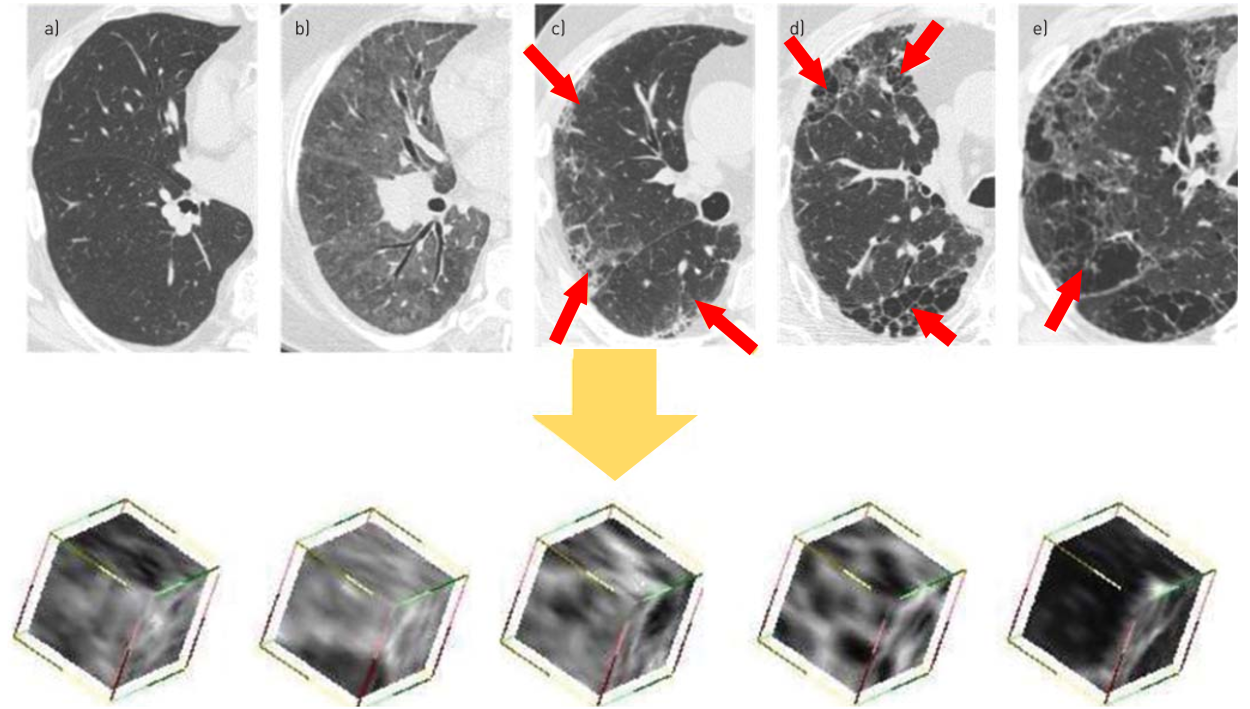
\includegraphics[height=3.0in]{QuantitativeAnalysis/Image/CALIPERPatterns.png}
  \caption{Computed tomography images demonstrating appearance and various visual manifestations of idiopathic pulmonary fibrosis: a) normal, b) ground glass, c) reticular changes (arrows), d) honeycombing (arrows) and e) emphysema (arrow). In training datasets, the consensus of four thoracic radiologists was used to identify multiple VOIs corresponding to normal, ground-glass density, reticular abnormalities, honeycombing and emphysema. Reproduced from \citep{maldonado2013automated}.}
  \label{fig:CALIPERPatterns}
\end{figure*}

Pre-processing was conducted before the eventual classification of the pulmonary parenchyma. This required segmentation of anatomic lung regions. The lungs were initially segmented using a adaptive density-based morphology (thresholding) method \citep{hu2001automatic}. Airways were segmented by thresholding combined with 3D growing processing and vessels were segmented by enhancement filter based on Hessian matrix \citep{sato2000tissue}, then the final lung segments were extracted. 

The volumetric detection and classification of pulmonary parenchyma by CALIPER uses a sliding window supervised classification scheme based on histogram signature mapping techniques \citep{zavaletta2007high}. This classification technique is trained by expert radiologist via consensus assessment of pathologically confirmed datasets, which are obtained from the Lung Tissue Research Consortium (LTRC). LTRC is a resource program sponsored by the NIH/NHLBI that provides clinical and physiologic data of human lung tissues to qualified investigators for use in their research and help investigators develop a better understanding of lung disease. The central part of the classification scheme is the selection of a set of expert-labled \gls{vois} as the training data for a classifier. The training data used in CALIPER was numbers of 15*15*15-voxel VOIs acquired from HRCT scans of subjects with proven pathological diagnosis of interstitial lung disease (ILD) or emphysema from the LTRC repository. These VOIs were selected through independent analysis by four experienced thoracic radiologists from CT scans, with instructions and criterion to determine if the visual appearance should represent normal, emphysema or one of the characteristic lung fibrosis CT patterns: honeycomb, reticular or ground-glass \citep{maldonado2013automated,bartholmai2013quantitative}.

The VOIs with agreement on the class of abnormality by all four radiologists were using as exemplars to determine canonical histogram signatures of the CT patterns of visual abnormality by automatic cluster affinity techniques. Quantitative discriminability of a series of pairwise dissimilarity metrics based on the VOI histograms was tested using \gls{mds}. \gls{cvm}, which was found to be most consistent with the expert groupings, was selected as the dissimilarity metric to train CALIPER. For each of the parenchymal voxel need to be classified, the local histograms of its neighbouring $15 \times 15 \times 15$ voxels were compared against the histograms of the exemplars identified in the training phase. A CVM dissimilarity measure was used in the comparison and the fundamental type of the exemplar (N,R,H,G or emphysema) with the lowest CVM was assigned as the parenchymal CT pattern to this classified voxel. The parenchymal voxels identified as vessel structures were classified as normal pattern. Figure \ref{fig:CALIPERResults} shows a representative dataset with axial, coronal and sagittal sections of a CT lung volume where every voxel of the parenchyma is characterized and color coded into one of the parenchymal patterns (N, R, H, G, and mild, moderate and severe LAA). 

\begin{figure*}[htbp]
  \centering 
  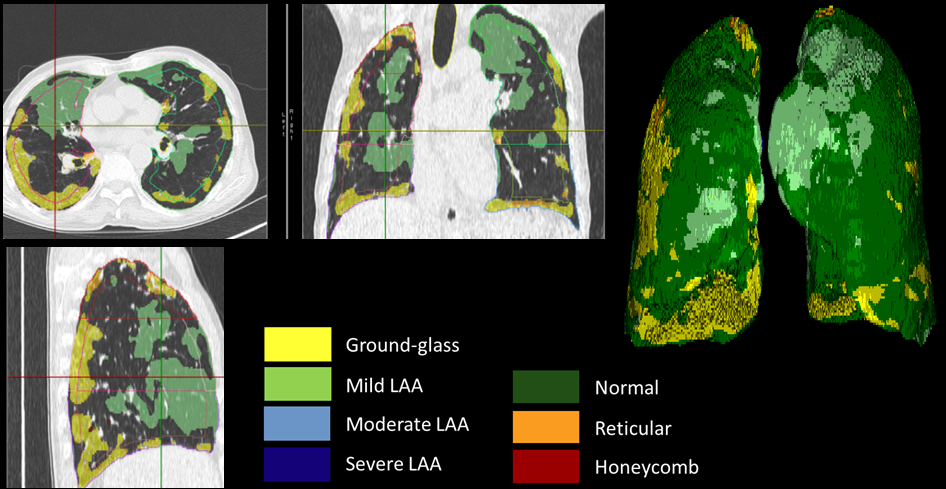
\includegraphics[height=2.9in]{QuantitativeAnalysis/Image/CALIPERResults.png}
  \caption{Color labelled classification result of one subject diagnosed with IPF by CALIPER.  (a) Transverse plane. (b) Coronal plane. (c) Sagittal plane. (d) 3D color labelled lung.}
  \label{fig:CALIPERResults}
\end{figure*}

%%%%%%%%%%%%%%%%%%%%%%%%%%%%%%%%%%
\subsubsection{Normalization of classified data} \label{DataNormalization}
Lung surface data and fissure surface data were acquired using the lobe segmentation method introduced in Chapter 3. A bi-cubic Hermite finite element surface mesh was fitted to the shape of the lung and its fissures via a least squares fit (https://www.cmiss.org). The details of generation of lobe data and lobe mesh can be seen in Chapter 3, Section \ref{ShapeModelGeneration}.

There is lung shape variation between different subjects and often between clinical images obtained at different times, as well as variation in the extent to which a patient inhales for imaging, even with careful training. Thus, classified volumetric lung data was then mapped to a statistical shape model (SSM) of the ''normal'' older human lung to provide a consistent mapping of tissue abnormalities between and within individuals to a same lung shape. The steps for the construction of SSM were introduced in Chapter 3, Section \ref{ShapeModelGeneration}. In this chapter we used 35 normal old subjects chosen from the human aging cohort (AGING) as the training dataset for PCA analysis to build SSM. The SSM used for mapping data is the average mesh of the lung lobe which derived from these 35 training subjects, and it provides a description of a statistical mean lung and fissure surface shape of old normal people.

In order to map the individual classified data to the SSM mesh, all of the classified data should be completely enclosed inside its fitted lobe surface mesh. The position of each point within the finite element mesh was defined locally in each element of the mesh by $\xi_{i}$, for i=1,..,3 with $0<\xi_{i}<1$. $\xi_{i}$ location denotes the local coordinates of the data point with respect to its element. The local coordinate $\xi_{i}$ was then used to calculate the global coordinates of the mapped data points using the following equation:

\begin{equation}
u(\xi_{i}) = \sum_{n=1}^{N} \psi_n(\xi_{i})u_n
\end{equation}
where $u_n$ is a vector of N element nodal parameters of the SSM lobe mesh associated with the interpolation functions $\psi_{n}$. Figure \ref{fig:MappingResult} shows the mapped classification data for a single subject.

\newgeometry{bottom=4cm} %set the left margin of page
\begin{landscape}
\begin{figure}[htbp]
\begin{subfigure}{6.5cm}
    \makebox[60pt]{\raisebox{50pt}{\rotatebox[origin=c]{0}{\minibox{Classified\\ data}}}}%
    \sbox0{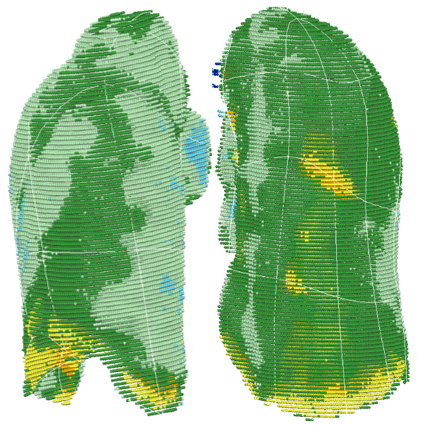
\includegraphics{QuantitativeAnalysis/Image/ClassifiedData_Time1.png}}% get image width, trim={<left> <lower> <right> <upper>}
    \begin{overpic}[height=1.73in,trim={{.0\wd0} {.0\wd0} {.0\wd0} {.0\wd0}},clip]{QuantitativeAnalysis/Image/ClassifiedData_Time1.png}
    \end{overpic}
    \makebox[60pt]{\raisebox{60pt}{\rotatebox[origin=c]{0}{\minibox{Mapped\\ data}}}}% \makebox:change left space, \raisebox: change upper space
    \begin{overpic}[height=1.83in,trim={{.0\wd0} {.0\wd0} {.0\wd0} {.0\wd0}},clip]{QuantitativeAnalysis/Image/MappedData_Time1.png}
    \end{overpic}
    \caption{Time point 1}
		\label{fig:MappingResult-a}
\end{subfigure}\hspace{0.3cm}
\begin{subfigure}{4.8cm}
    \sbox0{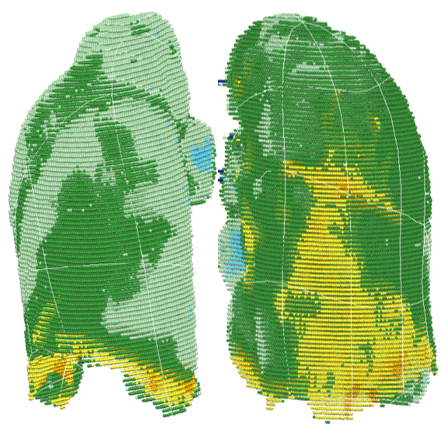
\includegraphics{QuantitativeAnalysis/Image/ClassifiedData_Time2.png}}% get image width, trim={<left> <lower> <right> <upper>}
    \begin{overpic}[height=1.7in,trim={{.0\wd0} {.0\wd0} {.0\wd0} {.0\wd0}},clip]{QuantitativeAnalysis/Image/ClassifiedData_Time2.png}
    \end{overpic}
    \begin{overpic}[height=1.88in,trim={{.0\wd0} {.0\wd0} {.0\wd0} {.0\wd0}},clip]{QuantitativeAnalysis/Image/MappedData_Time2.png}
    \end{overpic}
    \caption{Time point 2}
		\label{fig:MappingResult-b}
\end{subfigure}\hspace{0.3cm}
\begin{subfigure}{4.8cm}
    \sbox0{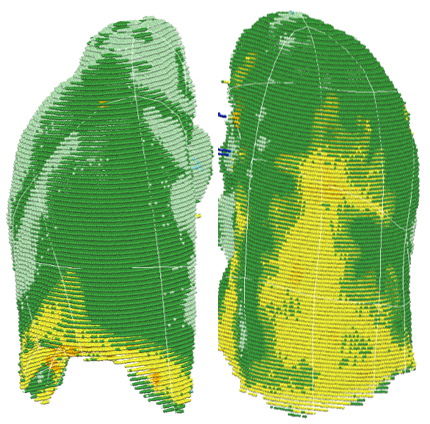
\includegraphics{QuantitativeAnalysis/Image/ClassifiedData_Time3.png}}% get image width, trim={<left> <lower> <right> <upper>}
    \begin{overpic}[height=1.67in,trim={{.0\wd0} {.0\wd0} {.0\wd0} {.0\wd0}},clip]{QuantitativeAnalysis/Image/ClassifiedData_Time3.png}
    \end{overpic}
    \begin{overpic}[height=1.9in,trim={{.0\wd0} {.0\wd0} {.0\wd0} {.0\wd0}},clip]{QuantitativeAnalysis/Image/MappedData_Time3.png}
    \end{overpic}
    \caption{Time point 3}
		\label{fig:MappingResult-c}
\end{subfigure}
\begin{subfigure}{2cm}
    \makebox[30pt]{\raisebox{100pt}{\rotatebox[origin=c]{0}{\minibox{\\}}}}
    \sbox0{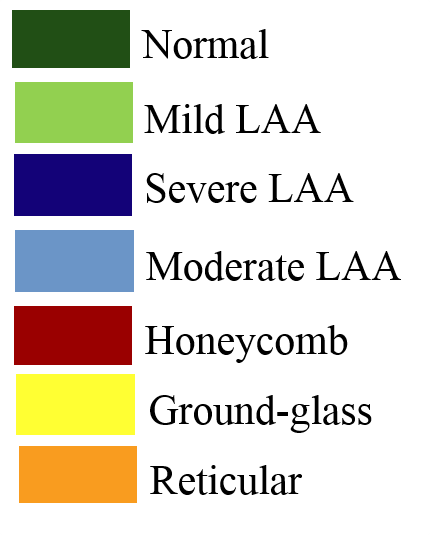
\includegraphics{QuantitativeAnalysis/Image/ClassifiedColor.png}}% get image width, trim={<left> <lower> <right> <upper>}
    \begin{overpic}[height=1.78in,trim={{.0\wd0} {.0\wd0} {.0\wd0} {.0\wd0}},clip]{QuantitativeAnalysis/Image/ClassifiedColor.png}
    \end{overpic}
\end{subfigure}
\caption{Classified data (top row) and mapped data (bottom row) of three time points from one subject diagnosed with IPF. (a) The first time point, scan time: 0 month. (b) The second time point, scan time: 15 months. (c) The third time point, scan time: 20 months}
\label{fig:MappingResult}
\end{figure}
\end{landscape}
\restoregeometry

In order to distribute the data points uniformly throughout each lung, the gaps in the mapped data caused by the deformation from individual shape to SSM (shown in Figure \ref{fig:GapFilling-a}) were filled through matching their closest neighbor point among the classified data, to allow the further density and spatial distribution analysis of abnormalities. Briefly, the gaps of the mapped data were filled using the following steps: 

1. Mapped data were cut into a series of axial slices (shown in Figure \ref{fig:GapFilling-a}).

2. The lung mesh of average SSM was used as a mask to define the lung boundary. (shown in Figure \ref{fig:GapFilling-b}).

3. Morphological operations were applied to smooth the lung boundary, then lung mask was generated (shown in Figure \ref{fig:GapFilling-c}).

4. The gaps enclosed inside the lung mask were filled with the CT pattern color of its closest point among the classified data (shown in Figure \ref{fig:GapFilling-d}).

%Figure \ref{fig:NormalizationResult} shows the slices with gaps and the slices after gap filling of three time points at the same position of lung.

\begin{figure*}[htbp] 
\centering
\begin{subfigure}{.28\linewidth}% set image scale
  \sbox0{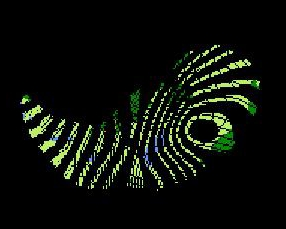
\includegraphics{QuantitativeAnalysis/Image/GapFilling1.jpg}} 
  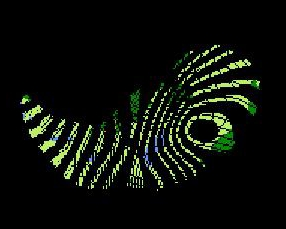
\includegraphics[width=\linewidth,trim={{.0\wd0} {.0\wd0} {.0\wd0} {.0\wd0}},clip]{QuantitativeAnalysis/Image/GapFilling1.jpg} %trim={<left> <lower> <right> <upper>}, set the cut scale
  \caption{Axial slices with gaps\\ \quad}
  \label{fig:GapFilling-a} 
\end{subfigure} 
%\vspace{.3in} % control space between the upper context and figure
\hspace{.5in} % control space between two figures
\begin{subfigure}{.28\linewidth}% set image scale
  \sbox0{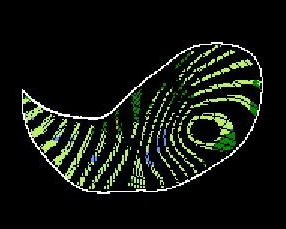
\includegraphics{QuantitativeAnalysis/Image/GapFilling2.jpg}}
  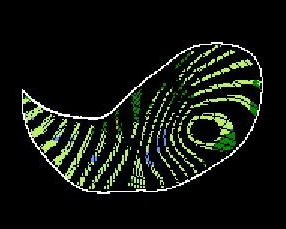
\includegraphics[width=\linewidth,trim={{.0\wd0} {.0\wd0} {.0\wd0} {.0\wd0}},clip]{QuantitativeAnalysis/Image/GapFilling2.jpg}
  \caption{Lung boundary\\ \quad}
  \label{fig:GapFilling-b} 
\end{subfigure}
\hspace{.5in}
\begin{subfigure}{.28\linewidth}% set image scale
  \sbox0{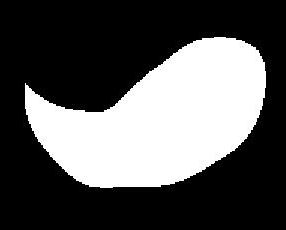
\includegraphics{QuantitativeAnalysis/Image/GapFilling3.jpg}}
  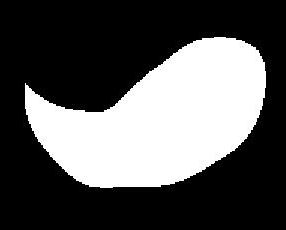
\includegraphics[width=\linewidth,trim={{.0\wd0} {.0\wd0} {.0\wd0} {.0\wd0}},clip]{QuantitativeAnalysis/Image/GapFilling3.jpg}
  \caption{Lung mask}
  \label{fig:GapFilling-c} 
\end{subfigure}
%\vspace{.3in} % control space between the upper context and figure
\hspace{.5in} % control space between two figures
\begin{subfigure}{.28\linewidth}% set image scale
  \sbox0{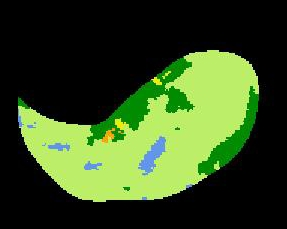
\includegraphics{QuantitativeAnalysis/Image/GapFilling4.jpg}}
  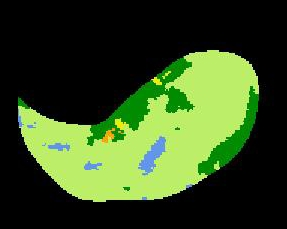
\includegraphics[width=\linewidth,trim={{.0\wd0} {.0\wd0} {.0\wd0} {.0\wd0}},clip]{QuantitativeAnalysis/Image/GapFilling4.jpg}
  \caption{Gap filled slice}
  \label{fig:GapFilling-d} 
\end{subfigure}
\caption{Diagram of gap filling steps within the mapped data. (a) Get axial slices of mapped data (with gaps). (b) Define lung boundary (SSM defined). (c) Get lung mask. (d) Fill the gaps within lung mask.}
\label{fig:GapFilling}
\end{figure*}

%\begin{figure}[htbp]
%\begin{subfigure}{3.7cm}
    %\makebox[4pt]{\raisebox{50pt}{\rotatebox[origin=c]{0}{\minibox{\\}}}}%
    %\sbox0{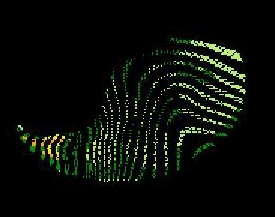
\includegraphics{QuantitativeAnalysis/Image/IPF6_Original_Slice65_1.jpg}}% get image width, trim={<left> <lower> <right> <upper>}
    %\begin{overpic}[height=1.2in,trim={{.0\wd0} {.0\wd0} {.0\wd0} {.0\wd0}},clip]{QuantitativeAnalysis/Image/IPF6_Original_Slice65_1.jpg}
    %\end{overpic}
    %\makebox[4pt]{\raisebox{87pt}{\rotatebox[origin=c]{0}{\minibox{\\}}}}%
    %\begin{overpic}[height=1.2in,trim={{.0\wd0} {.0\wd0} {.0\wd0} {.0\wd0}},clip]{QuantitativeAnalysis/Image/IPF6_Filled_Slice65_1.jpg}
    %\end{overpic}
    %\caption{Time point 1}
		%\label{fig:NormalizationResult-a}
%\end{subfigure}\hspace{.5in}
%\begin{subfigure}{3.7cm}
    %\makebox[4pt]{\raisebox{50pt}{\rotatebox[origin=c]{0}{\minibox{\\}}}}%
    %\sbox0{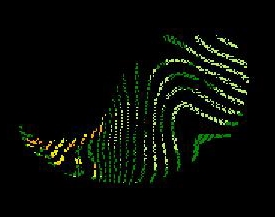
\includegraphics{QuantitativeAnalysis/Image/IPF6_Original_Slice65_2.jpg}}% get image width, trim={<left> <lower> <right> <upper>}
    %\begin{overpic}[height=1.2in,trim={{.0\wd0} {.0\wd0} {.0\wd0} {.0\wd0}},clip]{QuantitativeAnalysis/Image/IPF6_Original_Slice65_2.jpg}
    %\end{overpic}
		%\makebox[4pt]{\raisebox{87pt}{\rotatebox[origin=c]{0}{\minibox{\\}}}}%
    %\begin{overpic}[height=1.2in,trim={{.0\wd0} {.0\wd0} {.0\wd0} {.0\wd0}},clip]{QuantitativeAnalysis/Image/IPF6_Filled_Slice65_2.jpg}
    %\end{overpic}
    %\caption{Time point 2}
		%\label{fig:NormalizationResult-b}
%\end{subfigure}\hspace{.5in}
%\begin{subfigure}{3.7cm}
    %\makebox[4pt]{\raisebox{50pt}{\rotatebox[origin=c]{0}{\minibox{\\}}}}%
    %\sbox0{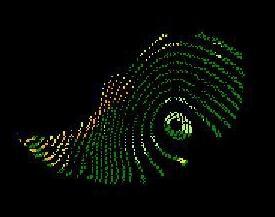
\includegraphics{QuantitativeAnalysis/Image/IPF6_Original_Slice65_3.jpg}}% get image width, trim={<left> <lower> <right> <upper>}
    %\begin{overpic}[height=1.2in,trim={{.0\wd0} {.0\wd0} {.0\wd0} {.0\wd0}},clip]{QuantitativeAnalysis/Image/IPF6_Original_Slice65_3.jpg}
    %\end{overpic}
		%\makebox[4pt]{\raisebox{87pt}{\rotatebox[origin=c]{0}{\minibox{\\}}}}%
    %\begin{overpic}[height=1.2in,trim={{.0\wd0} {.0\wd0} {.0\wd0} {.0\wd0}},clip]{QuantitativeAnalysis/Image/IPF6_Filled_Slice65_3.jpg}
    %\end{overpic}
    %\caption{Time point 3}
		%\label{fig:NormalizationResult-c}
%\end{subfigure}
%\caption{Axial slices with gaps (top row) and axial slices after gap filling (bottom row) of three time points from one subject diagnosed with IPF. (a) The first time point, scan date: 15/10/2012. (b) The second time point, scan date: 30/01/2014. (c) The third time point, scan date: 18/06/2014}
%\label{fig:NormalizationResult}
%\end{figure}

%%%%%%%%%%%%%%%%%%%%%%%%%%%%%%%%%%
\subsection{Tissue quantification of IPF lungs} \label{TissueQuantification}
\subsubsection{Density analysis}
The average density value of each classified CT pattern was calculated. Density is measured in Hounsfield units (HU) in a typical CT image, which corresponds linearly to the actual density of the imaged tissue. HU was calculated with the segmentation software PTK calibrated to values of approximately -1024 for air density, zero for water density, and over 40 for blood, bone, and other non-parenchymal tissue. The tissue density ($\rho$, $g/cm^3$ ) was then acquired at each voxel:

\begin{equation}
\rho = \frac{HU}{1024} + 1
\end{equation}

\noindent the average density of each CT pattern was then calculated from individual voxel density.

The density analysis result is shown in Figure \ref{fig:LungDensity} and Table \ref{tab:MeanDensity}. It can be seen that the average density of each CT pattern remains consistent and fluctuates only within a specific range over time. The ground-glass region has the highest average tissue density and emphysema has the lowest average tissue density. 

\begin{figure*}[htbp] 
\centering
\begin{subfigure}{.57\linewidth}% set image scale
  \sbox0{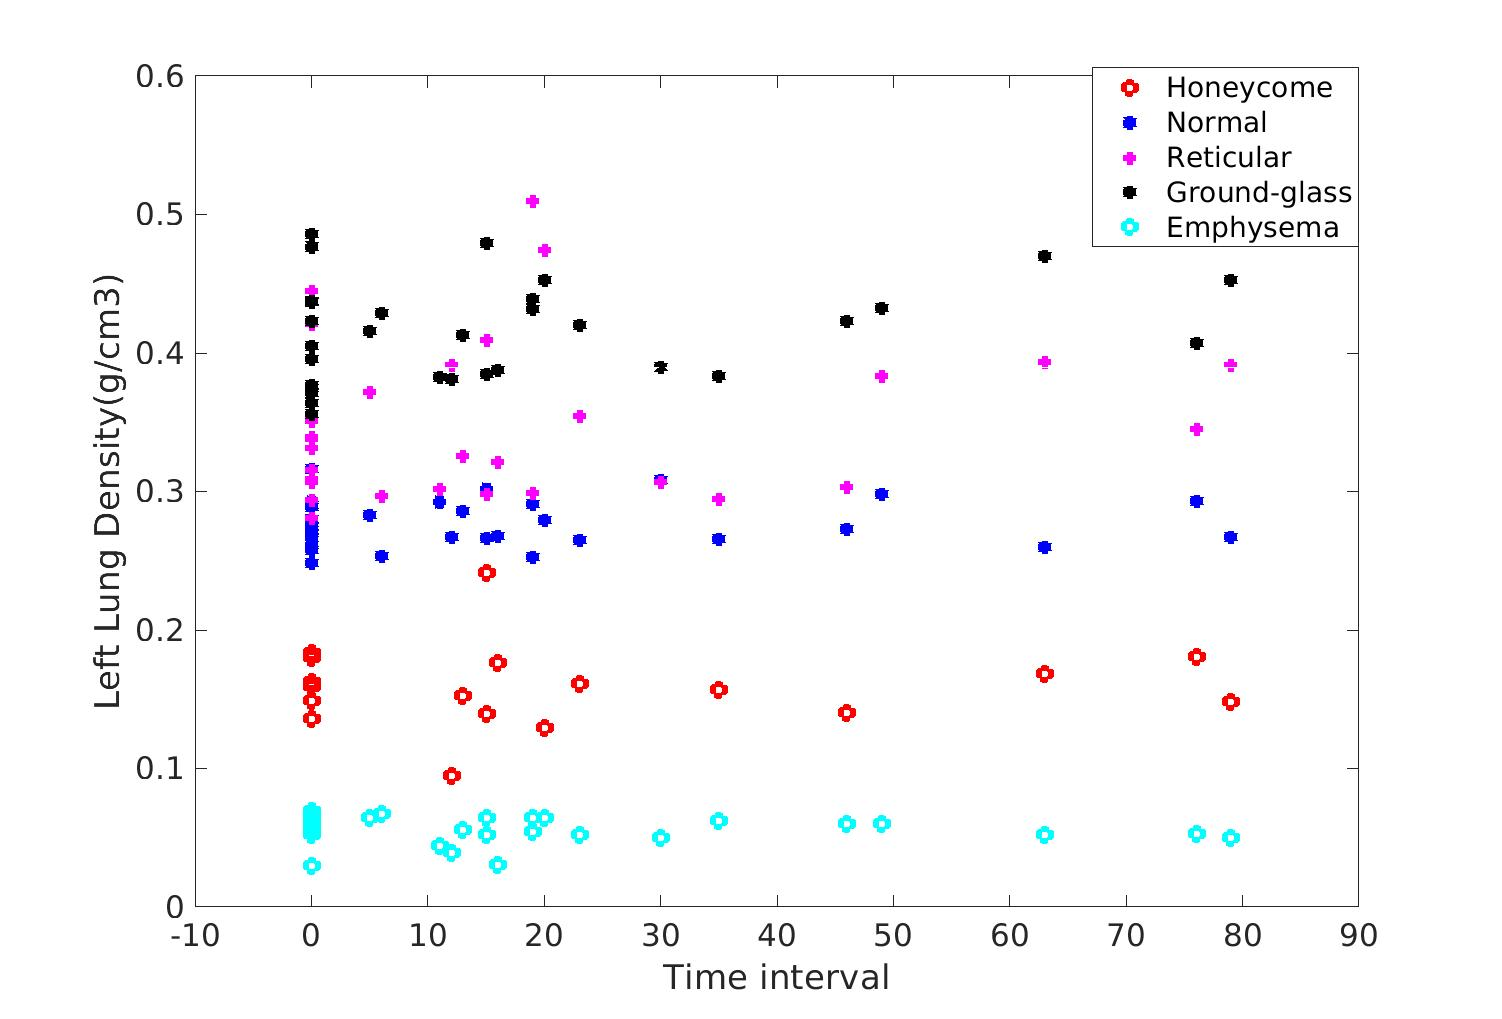
\includegraphics{QuantitativeAnalysis/Image/LeftLungDensity.jpg}} 
  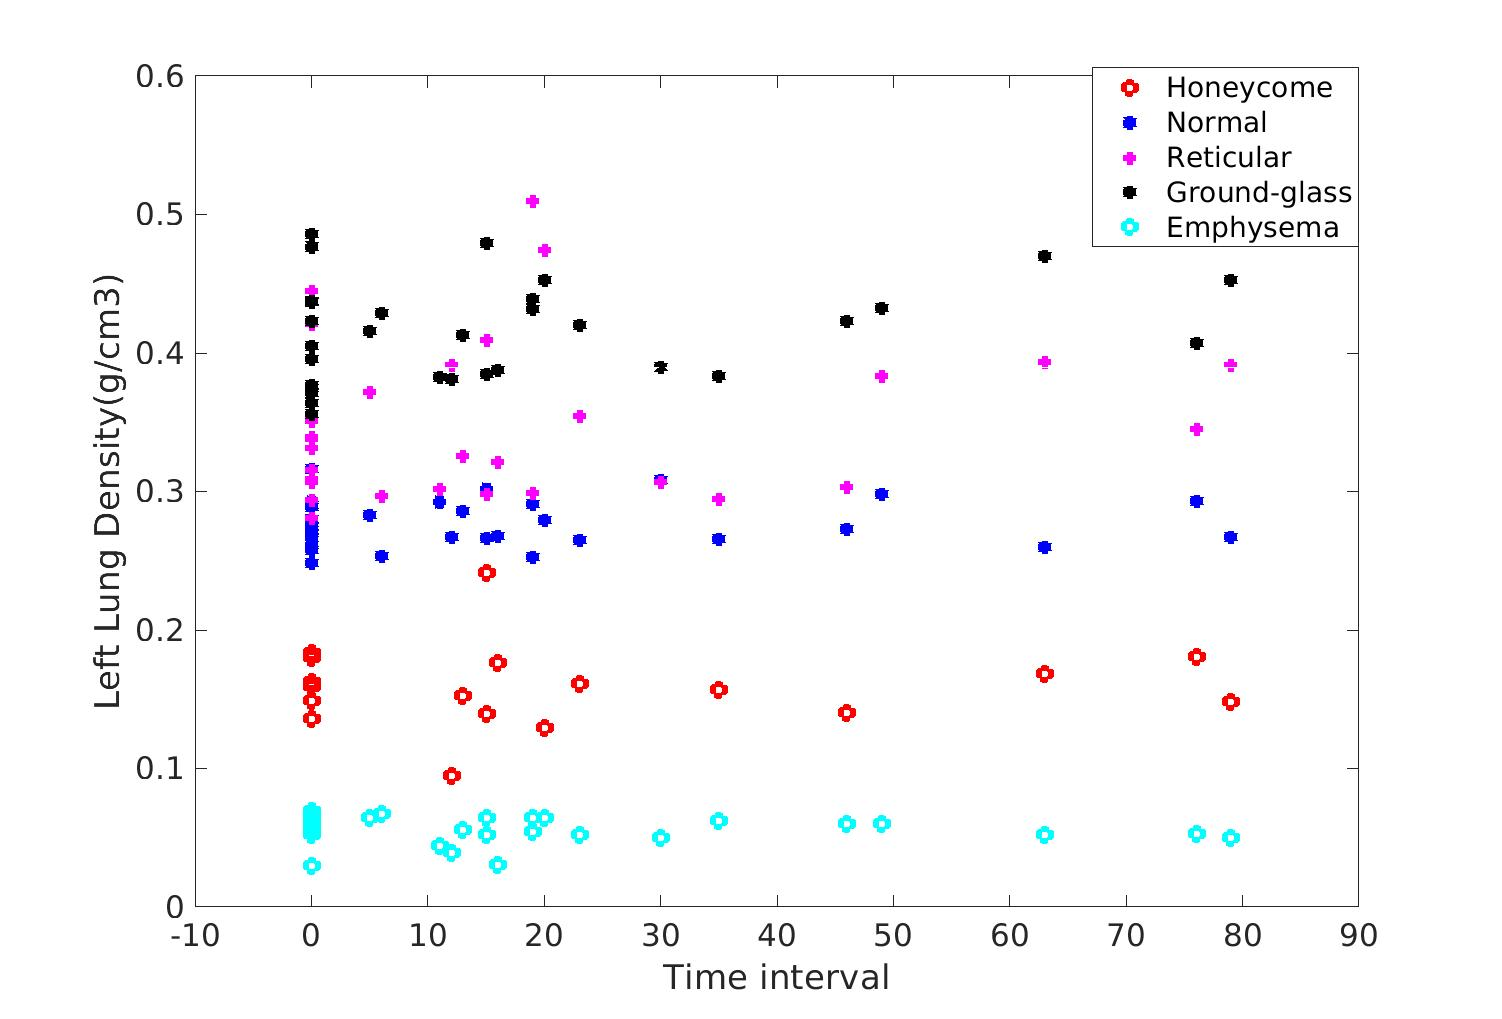
\includegraphics[width=\linewidth,trim={{.0\wd0} {.0\wd0} {.0\wd0} {.0\wd0}},clip]{QuantitativeAnalysis/Image/LeftLungDensity.jpg} %trim={<left> <lower> <right> <upper>}, set the cut scale
  \caption{Left lung tissue density}
  \label{fig:LungDensity-a} 
\end{subfigure} 
\hspace{.3in}
\begin{subfigure}{.57\linewidth}% set image scale
  \sbox0{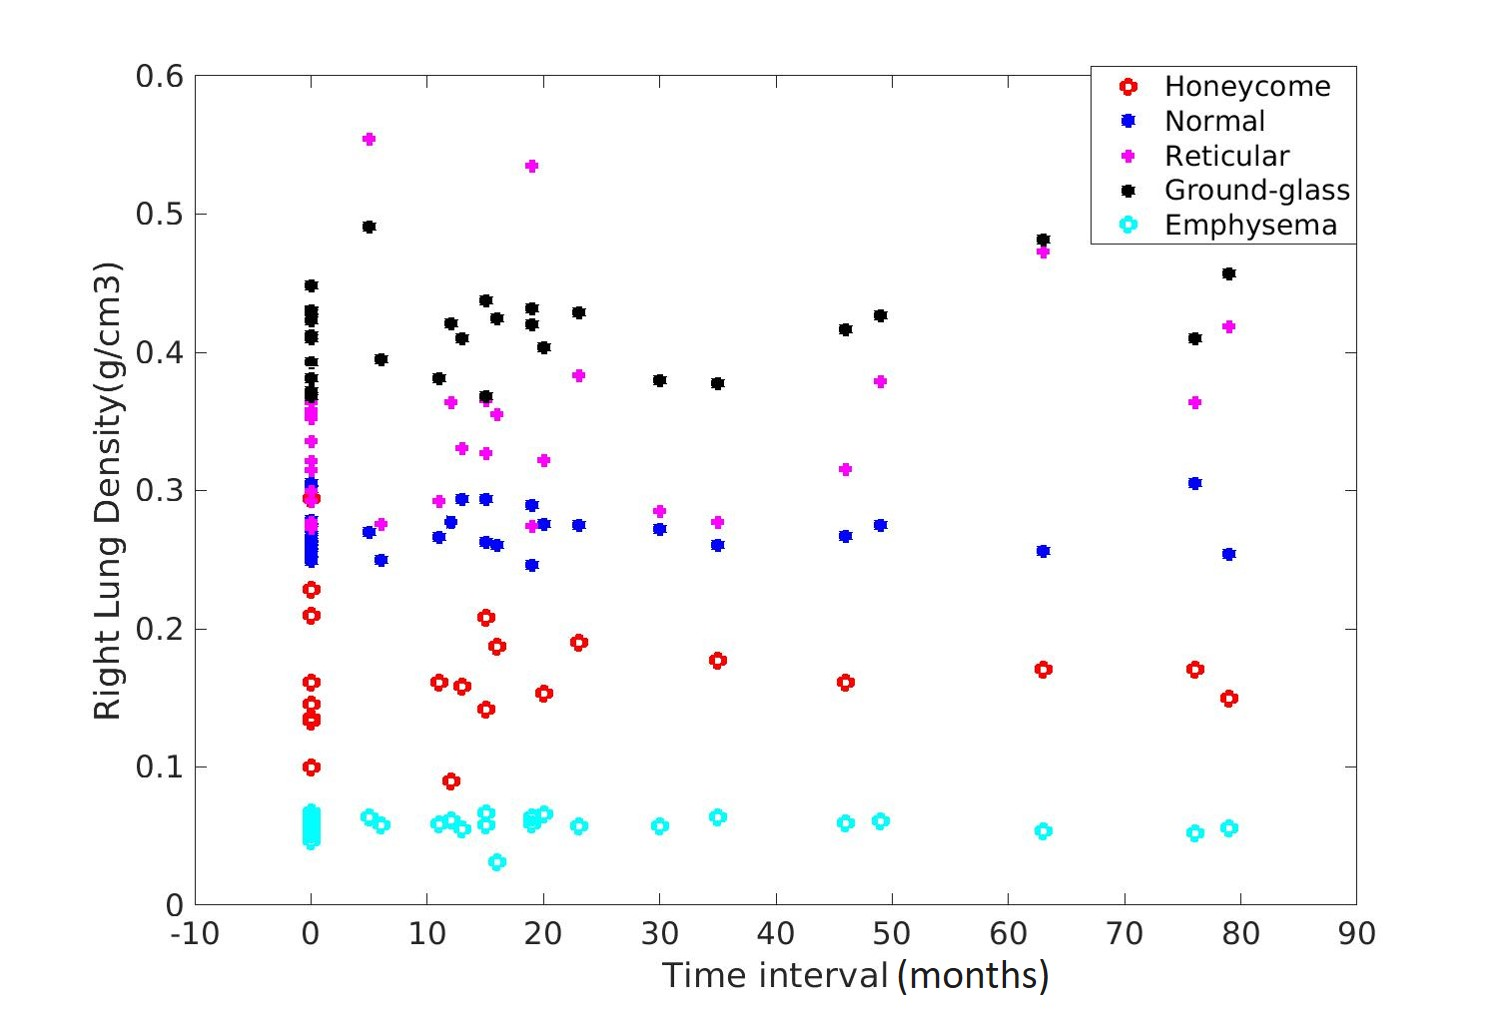
\includegraphics{QuantitativeAnalysis/Image/RightLungDensity.jpg}}
  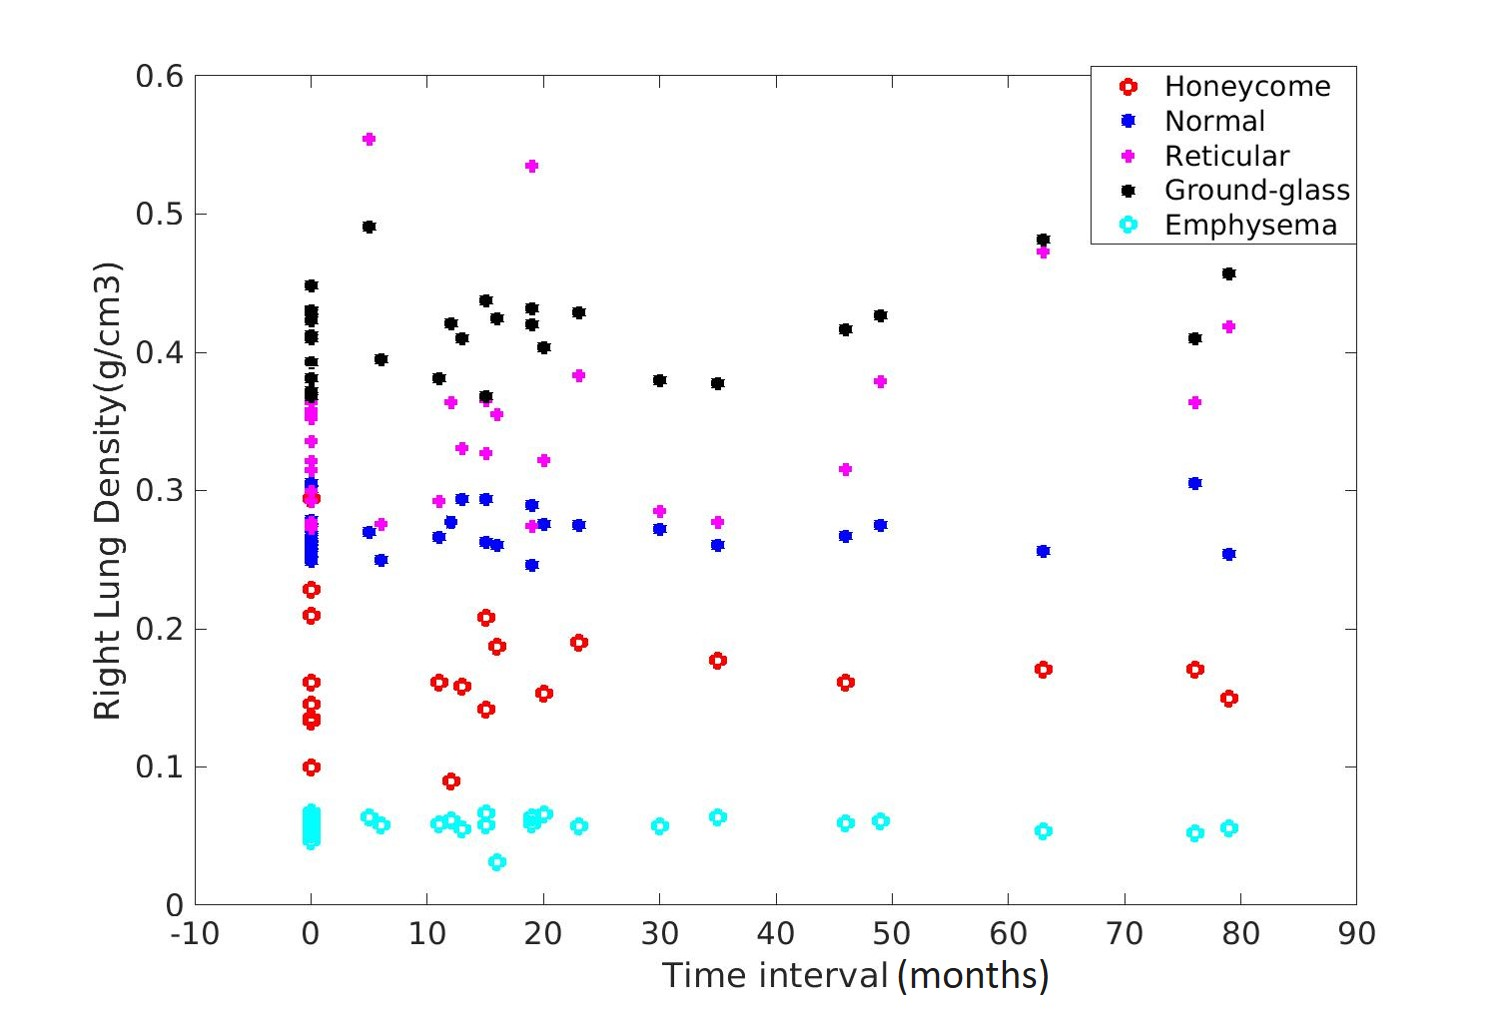
\includegraphics[width=\linewidth,trim={{.0\wd0} {.0\wd0} {.0\wd0} {.0\wd0}},clip]{QuantitativeAnalysis/Image/RightLungDensity.jpg}
  \caption{Right lung tissue density}
  \label{fig:LungDensity-b} 
\end{subfigure}
\caption{Average tissue density (g/cm3) of each CT pattern in IPF lungs. Each data point represents the average density of each patient. X axis represents the month interval of scan time for each patient, and ‘0’ represents the first scan for this patient. (a) Tissue density of left lung. (b) Tissue density of right lung.}
\label{fig:LungDensity}
\end{figure*}

\begin{table}[htbp]
\centering
\caption{Mean tissue density of each CT pattern for left and right lung (mean value $\pm$ standard deviation)}
\label{tab:MeanDensity}
\begin{tabular}{|l | c | c|}
\hline
& \bf{Mean tissue density (left lung)} & \bf{Mean tissue density (right lung)} \\ 
\hline
\bf{Normal} & 0.280$\pm$0.022 & 0.271$\pm$0.015 \\
\hline
\bf{Honeycomb} & 0.148$\pm$0.039 & 0.155$\pm$0.027 \\
\hline
\bf{Reticular} & 0.355$\pm$0.054 & 0.321$\pm$0.039 \\
\hline
\bf{Ground-glass} & 0.424$\pm$0.051 & 0.404$\pm$0.018 \\
\hline
\bf{Emphysema} & 0.080$\pm$0.014 & 0.082$\pm$0.016 \\
\hline
\end{tabular}
\end{table}

\subsubsection{Spatial distribution analysis}
Based on the criteria of IPF set forth by members of ATS and ERS, the diagnosis of IPF usually associates with the presence of a UIP pattern on HRCT (see details in Chapter 2, Section \ref{DiagnosisCriteria}). The distribution of UIP on HRCT is characteristically basal and peripheral (subpleural), though often patchy. Therefore, in order to quantitatively analyze the spatial distribution of IPF abnormalities, the spatial distribution of honeycomb, reticular, emphysema and ground-glass which represent typical UIP disease patterns on HRCT were measured focusing on the three following aspects: 

1. Basal-to apical: In the direction from base to apex, the volume percentage of each disease region was averaged in 5\% percent lung height (along the dorsoventral axis). 

Figure \ref{fig:DiseaseAgainstHeight} shows the percentage distribution against lung height (dorsoventral axis) of four characteristic CT patterns: ground-glass, reticular, honeycomb and emphysema for left and right lung. It can be seen from the result that ground-glass mainly locates in the basal part of lung. The percentage of ground-glass decreases gradually with the increasing of the lung height. In contrast, the percentage of emphysema trends toward increasing from lung base to apex. The reticular tissue is mainly distributed basallt area and apex area, but it seldomly appears in the middle part of lung. The distribution of honeycomb does not have a relationship with lung height.
\newpage

\begin{figure}[H] 
\centering
\begin{subfigure}{.4\linewidth}% set image scale
  \sbox0{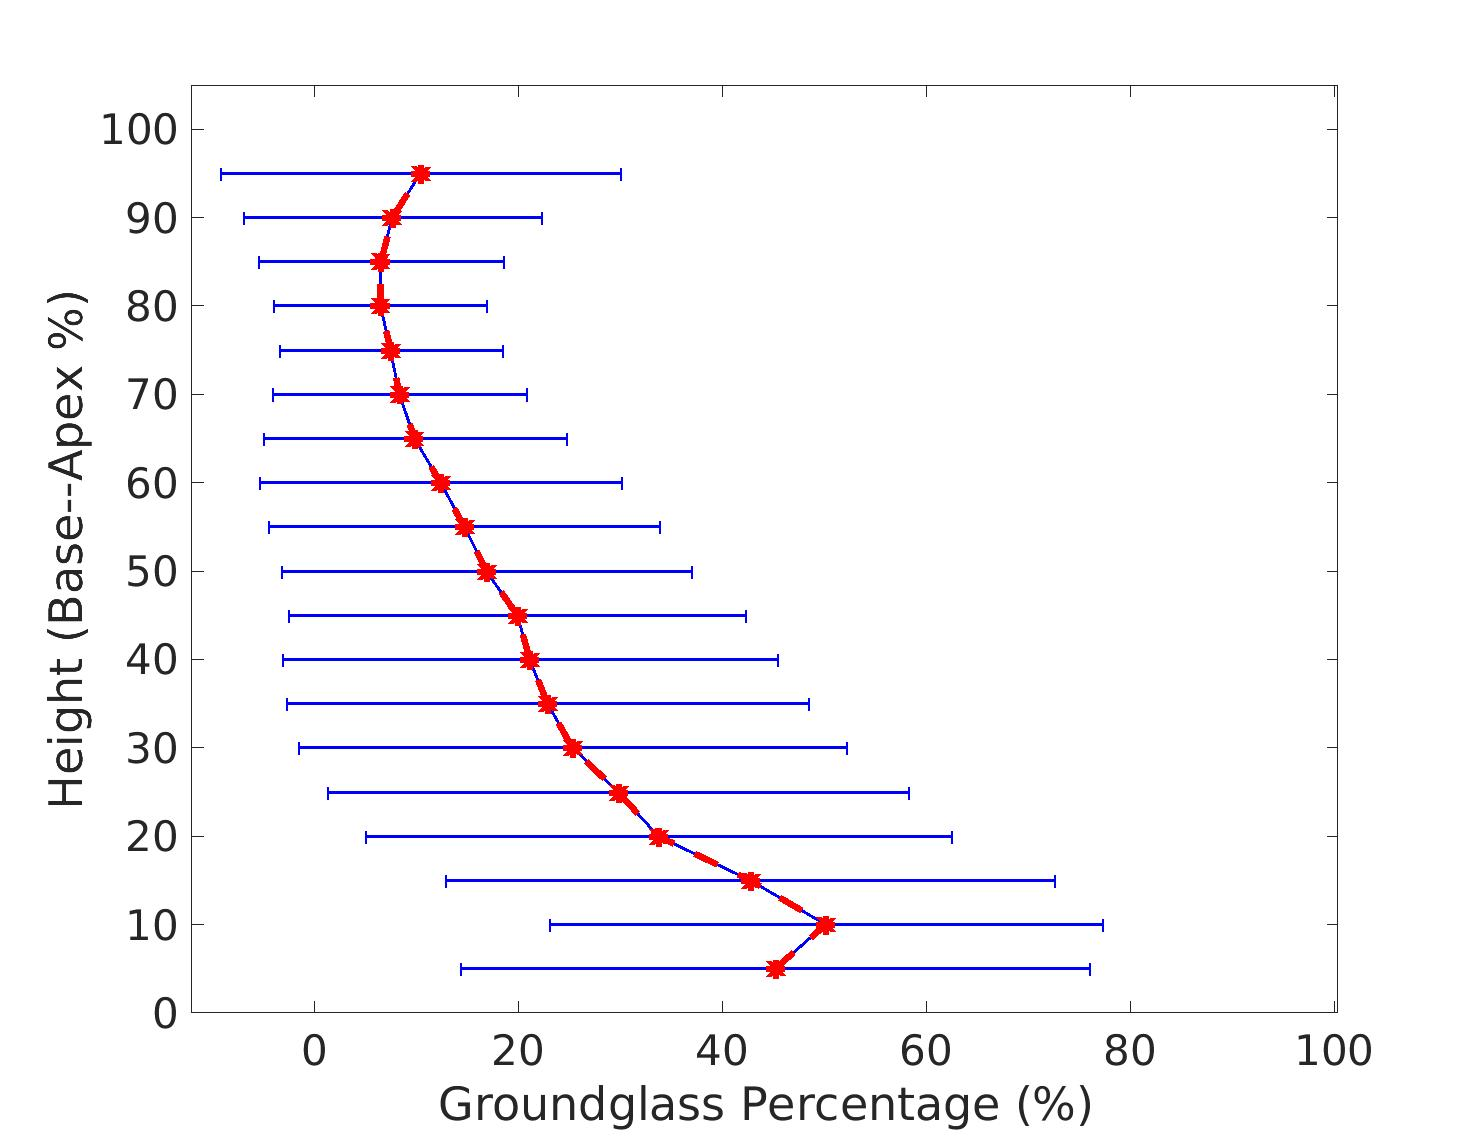
\includegraphics{QuantitativeAnalysis/Image/LeftLungGroundglassDiseaseAgainstHeight.jpg}} 
  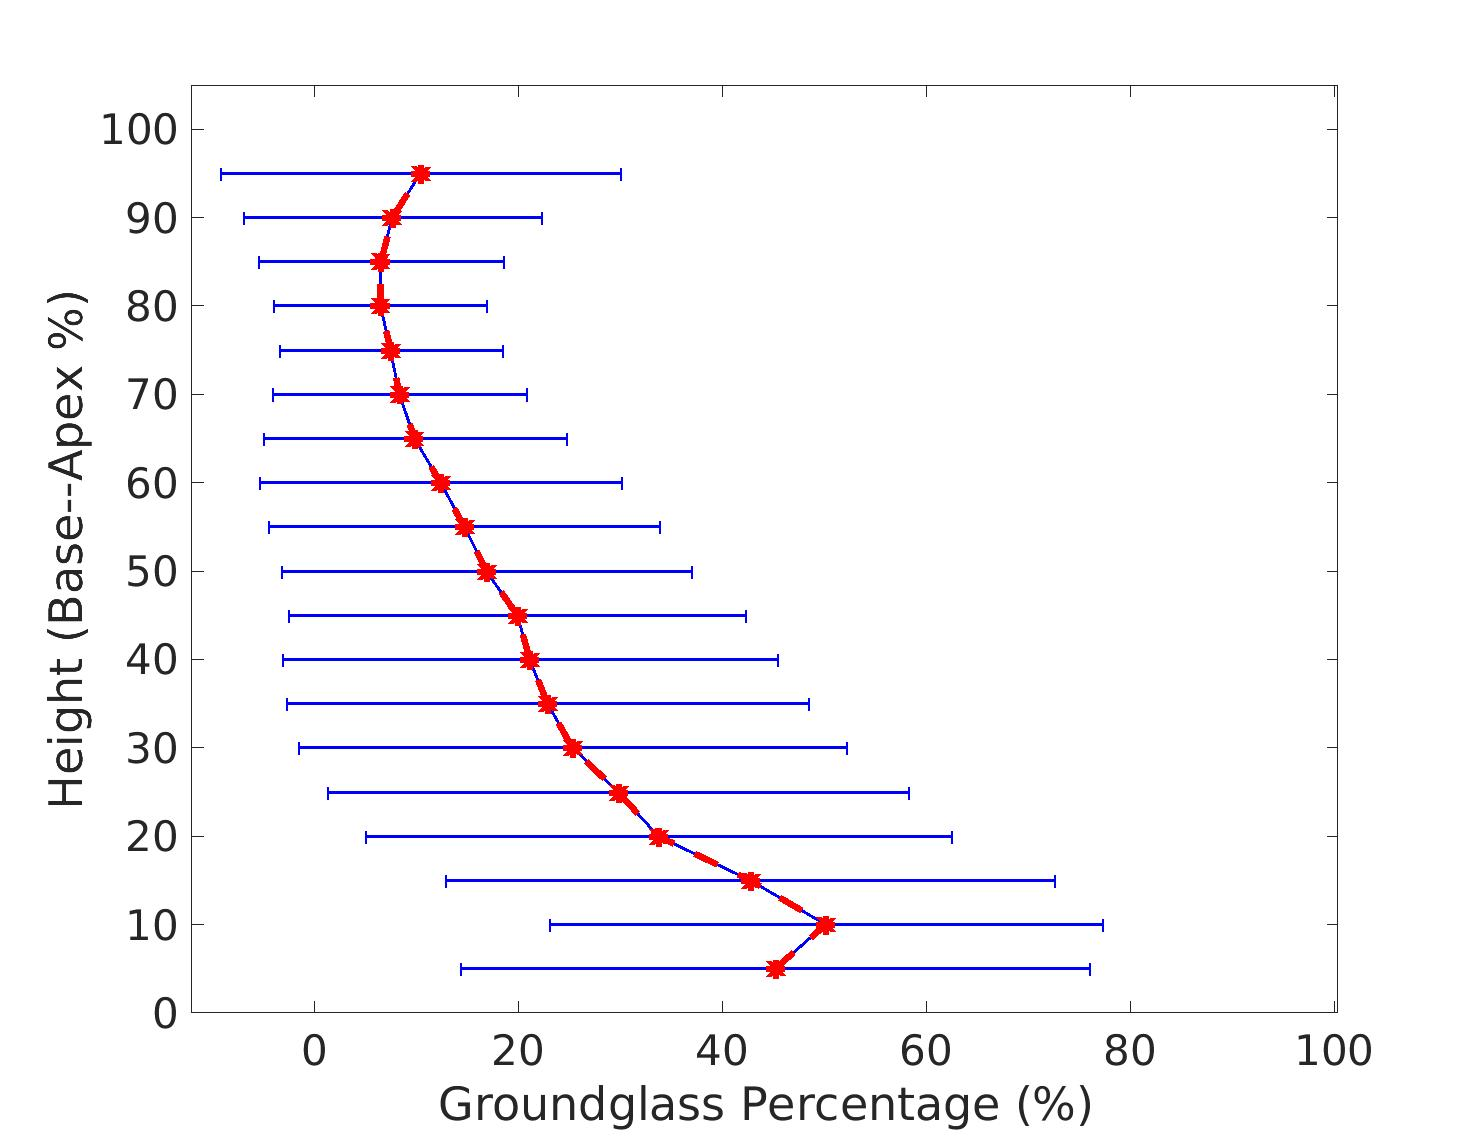
\includegraphics[width=\linewidth,trim={{.0\wd0} {.0\wd0} {.0\wd0} {.0\wd0}},clip]{QuantitativeAnalysis/Image/LeftLungGroundglassDiseaseAgainstHeight.jpg} %trim={<left> <lower> <right> <upper>}, set the cut scale
  \caption{}
  \label{fig:DiseaseAgainstHeight-a} 
\end{subfigure} 
\begin{subfigure}{.4\linewidth}% set image scale
  \sbox0{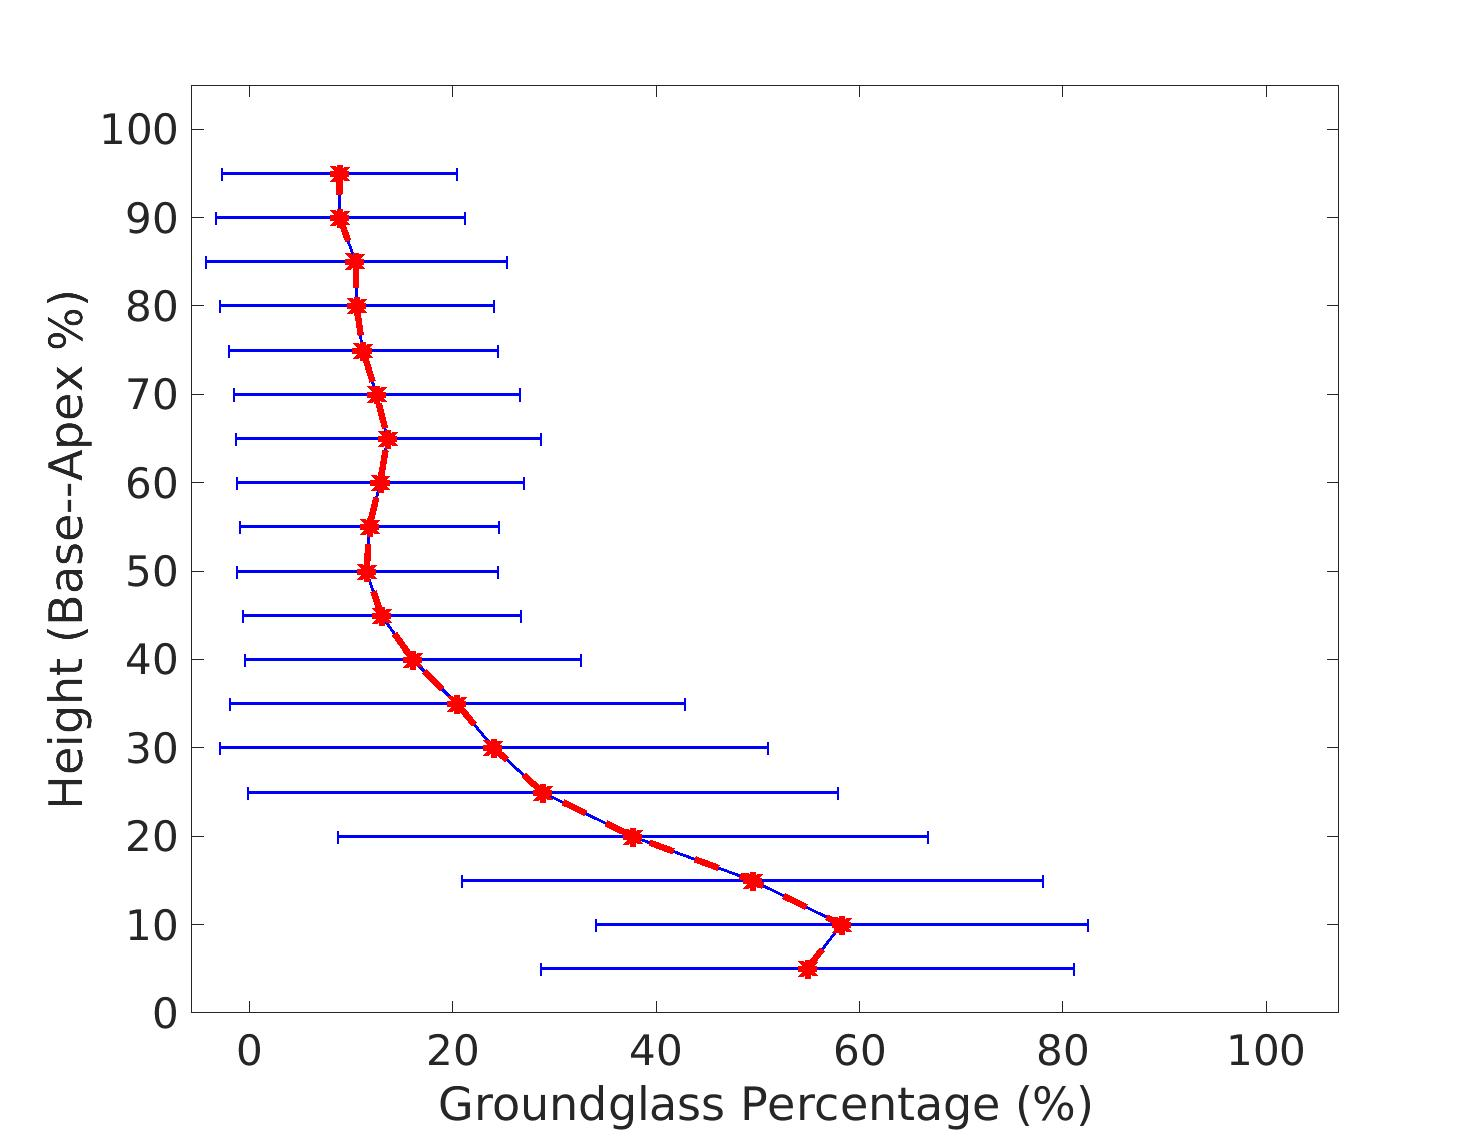
\includegraphics{QuantitativeAnalysis/Image/RightLungGroundglassDiseaseAgainstHeight.jpg}}
  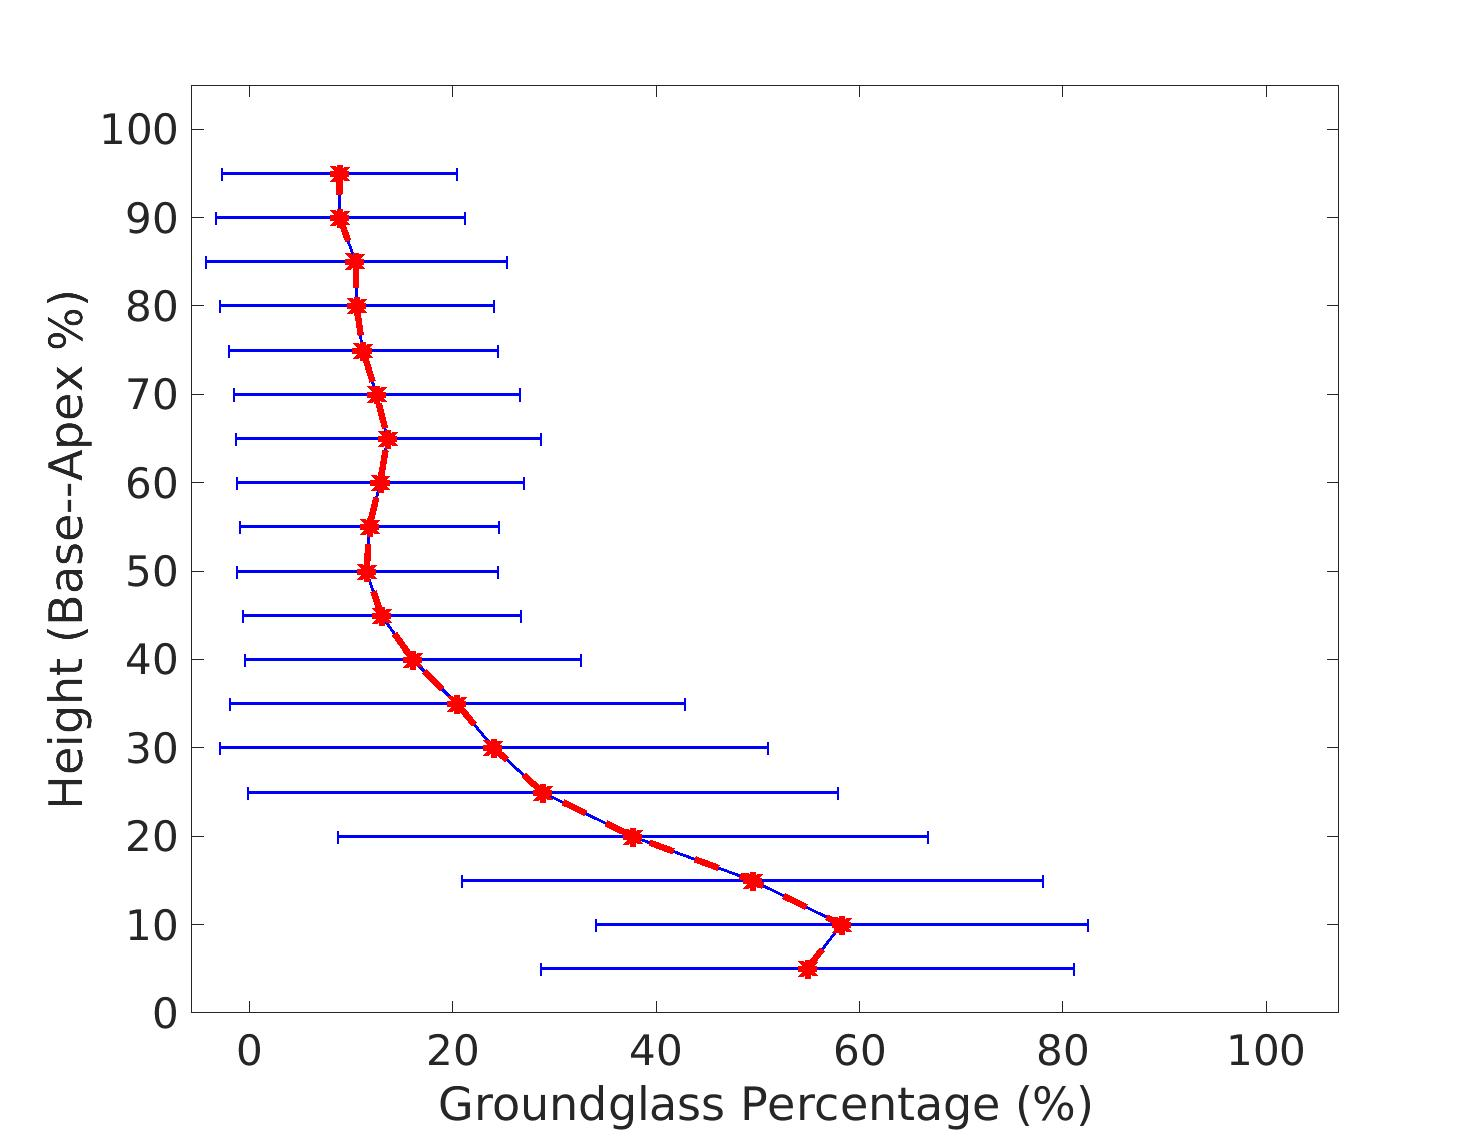
\includegraphics[width=\linewidth,trim={{.0\wd0} {.0\wd0} {.0\wd0} {.0\wd0}},clip]{QuantitativeAnalysis/Image/RightLungGroundglassDiseaseAgainstHeight.jpg}
  \caption{}
  \label{fig:DiseaseAgainstHeight-b}
\end{subfigure}
\begin{subfigure}{.4\linewidth}% set image scale
  \sbox0{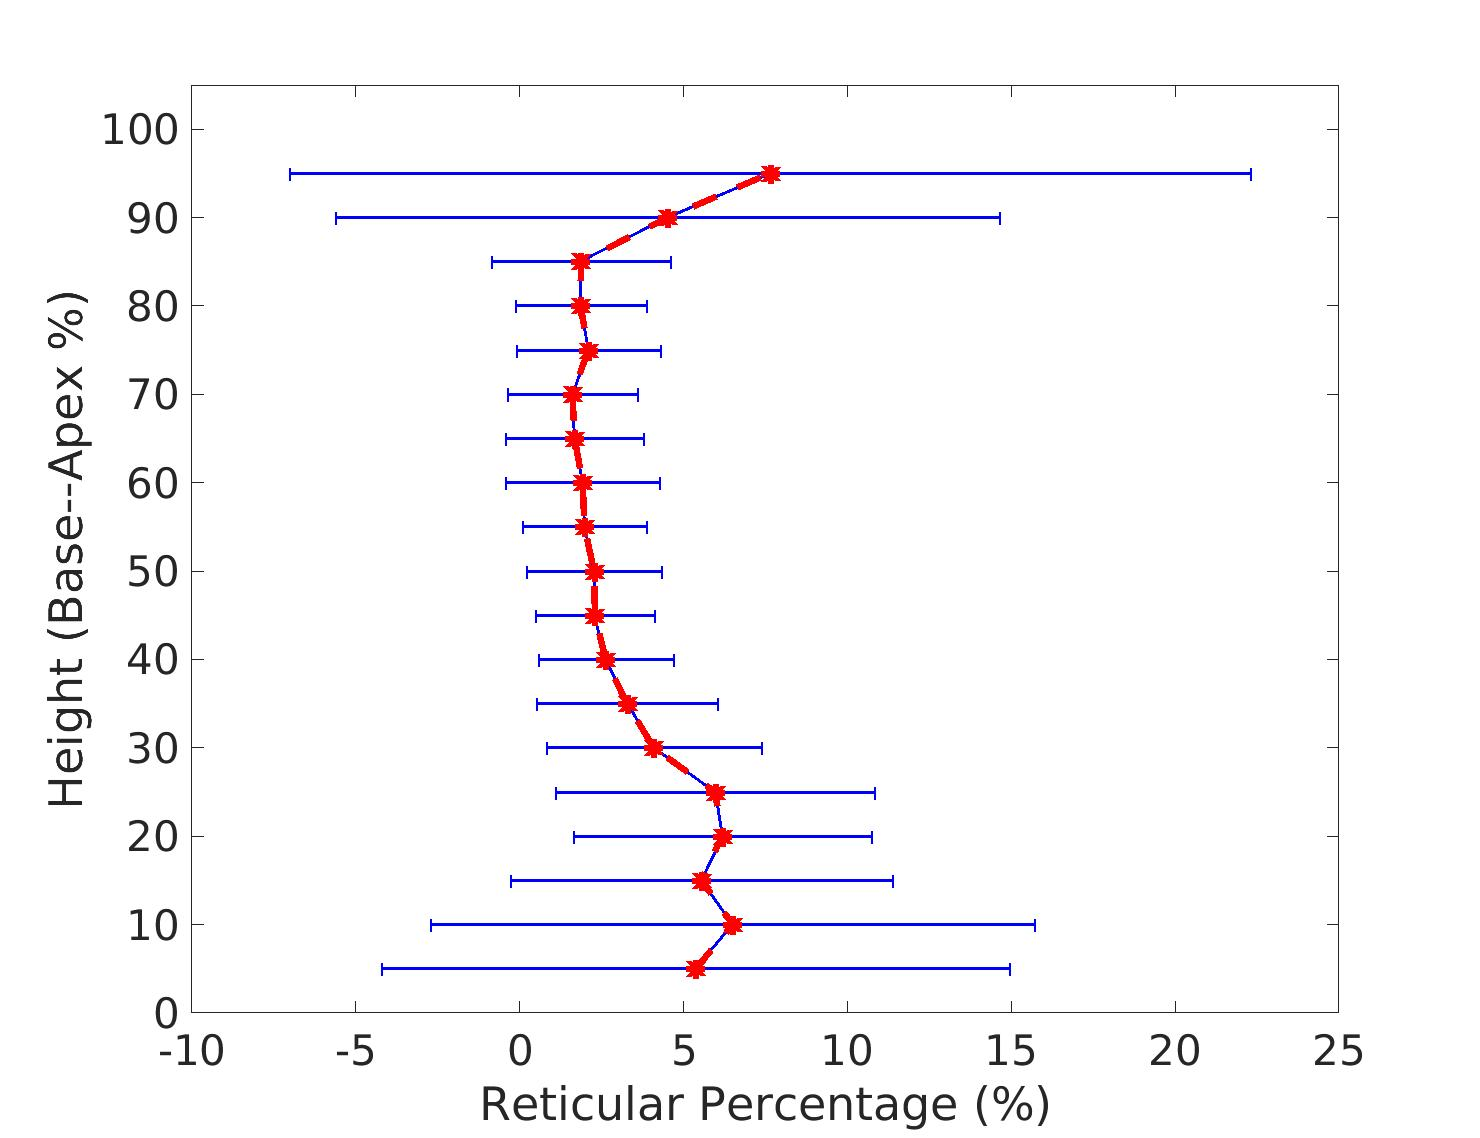
\includegraphics{QuantitativeAnalysis/Image/LeftLungReticularDiseaseAgainstHeight.jpg}} 
  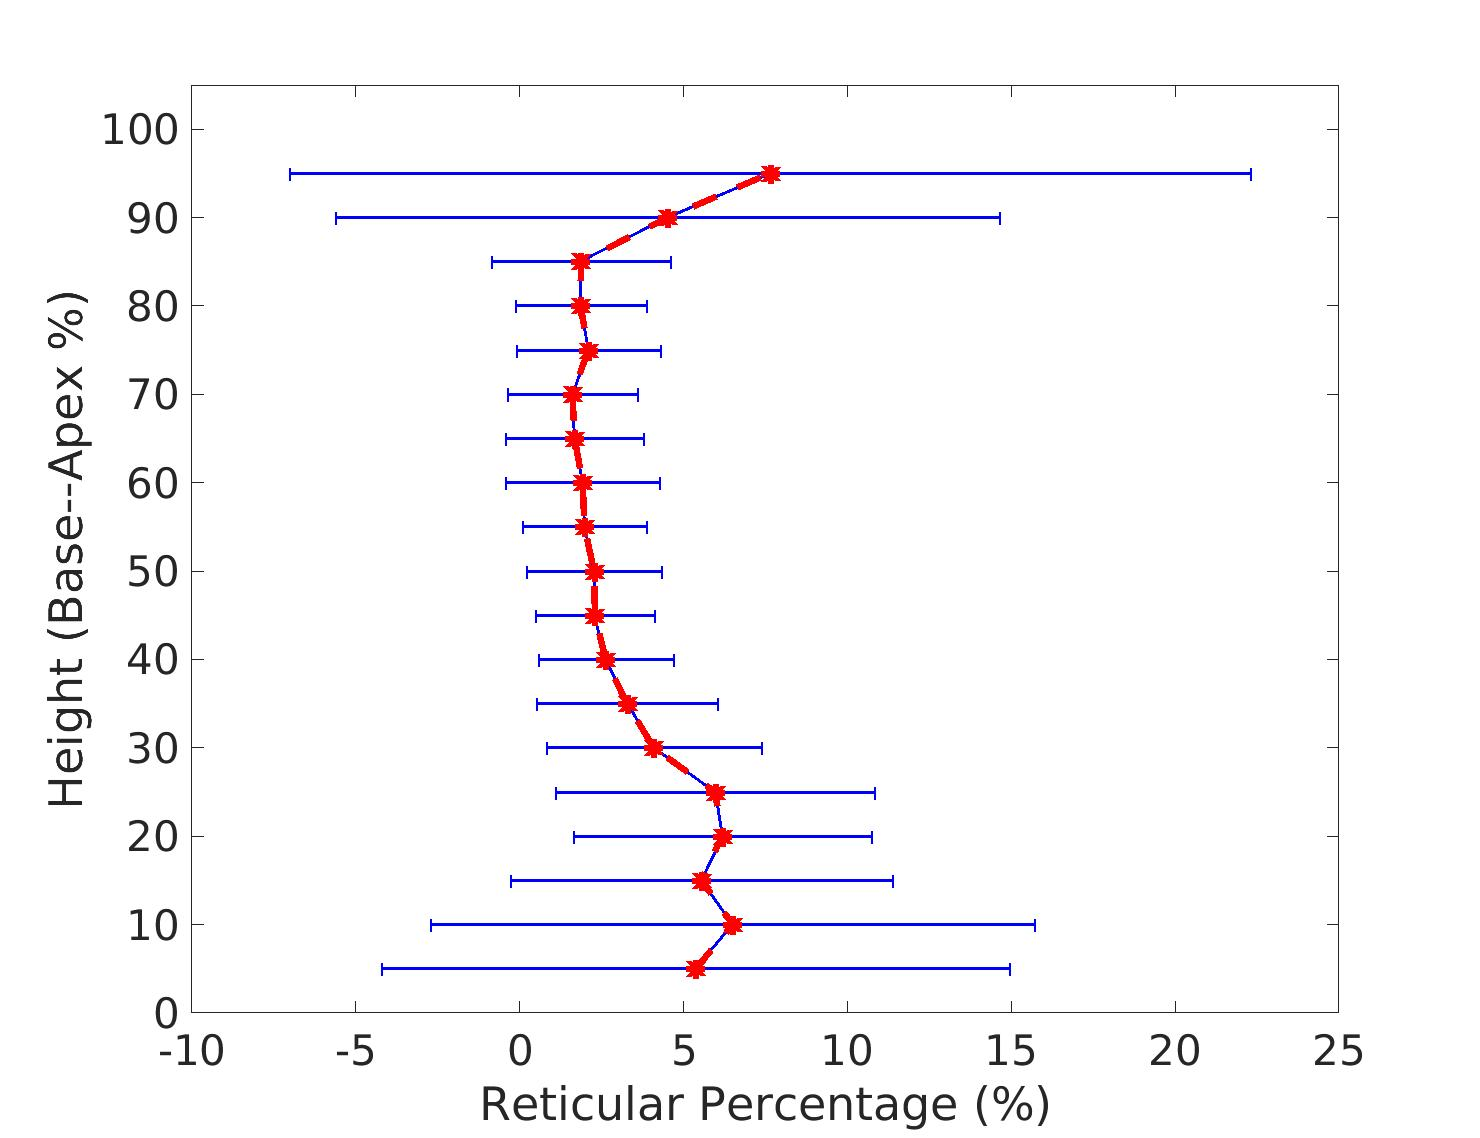
\includegraphics[width=\linewidth,trim={{.0\wd0} {.0\wd0} {.0\wd0} {.0\wd0}},clip]{QuantitativeAnalysis/Image/LeftLungReticularDiseaseAgainstHeight.jpg} %trim={<left> <lower> <right> <upper>}, set the cut scale
  \caption{}
  \label{fig:DiseaseAgainstHeight-c} 
\end{subfigure} 
\begin{subfigure}{.4\linewidth}% set image scale
  \sbox0{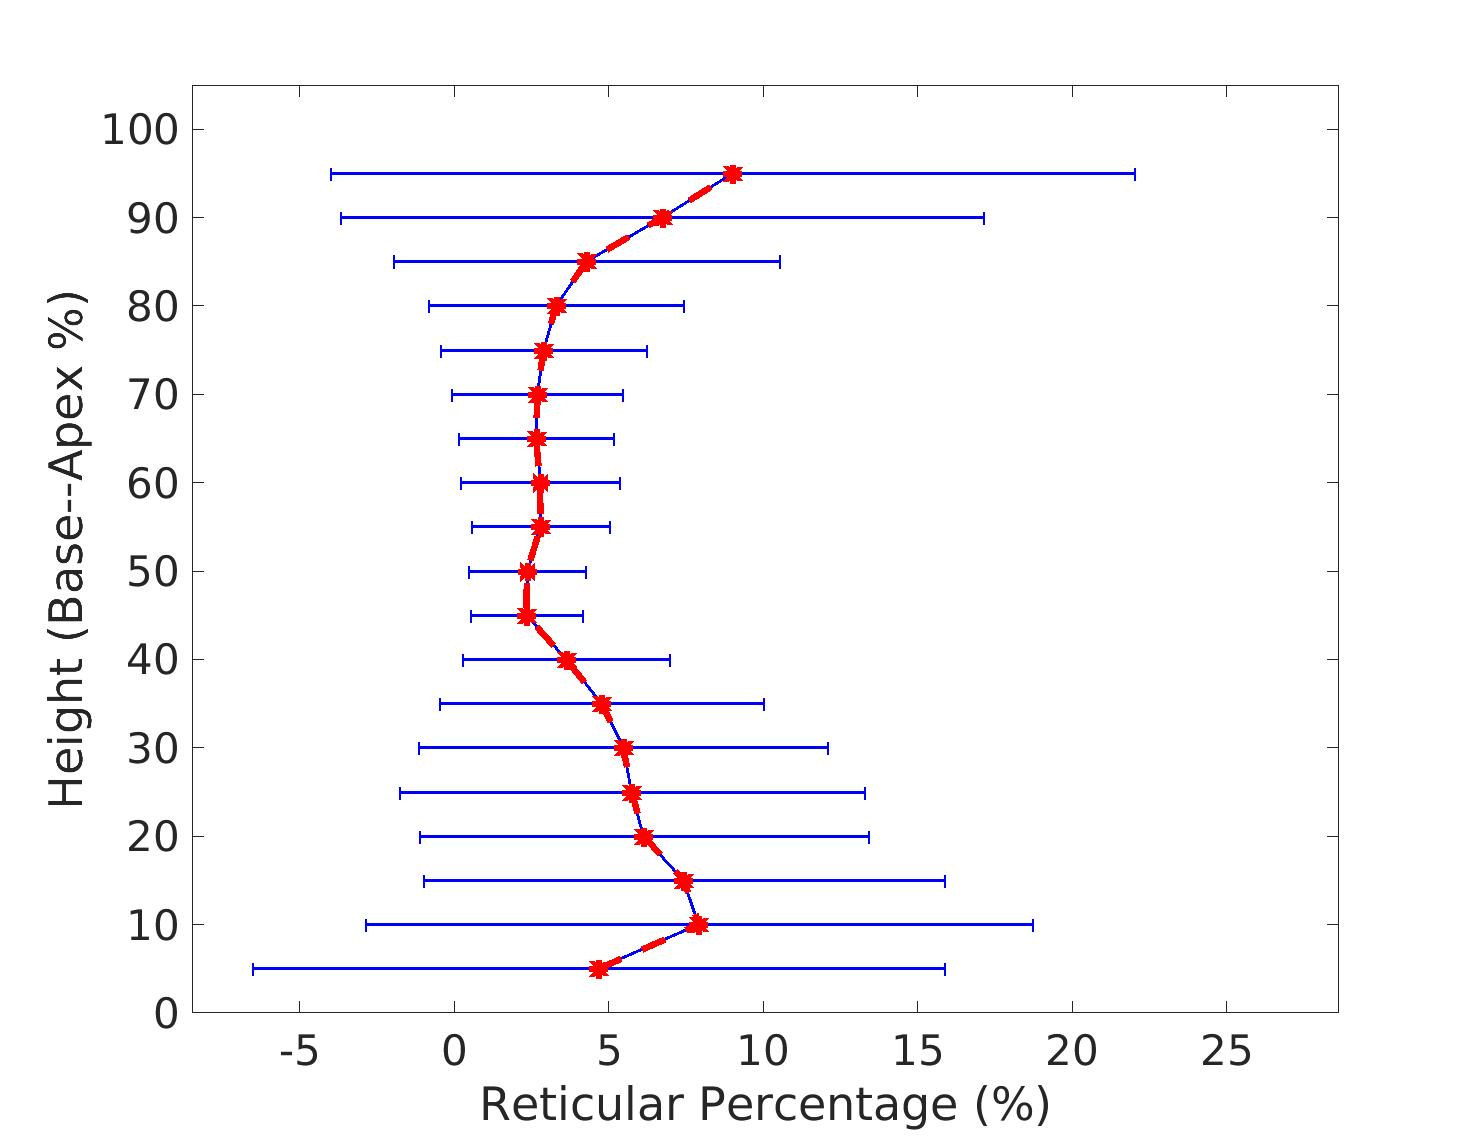
\includegraphics{QuantitativeAnalysis/Image/RightLungReticularDiseaseAgainstHeight.jpg}}
  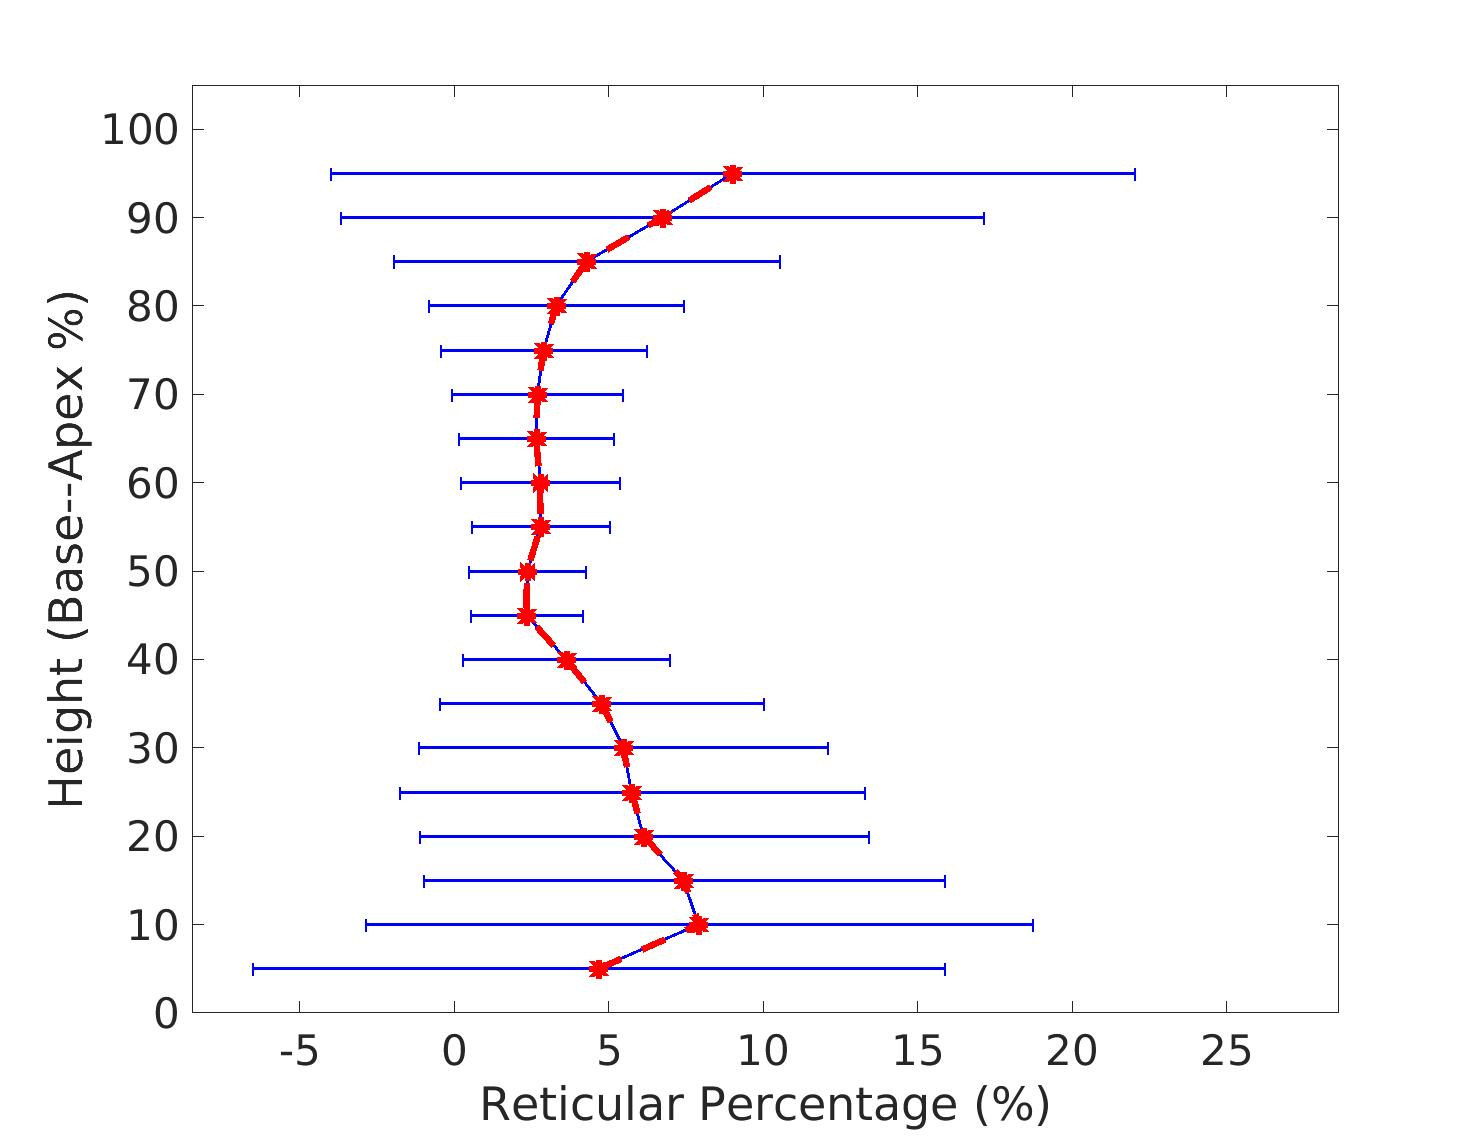
\includegraphics[width=\linewidth,trim={{.0\wd0} {.0\wd0} {.0\wd0} {.0\wd0}},clip]{QuantitativeAnalysis/Image/RightLungReticularDiseaseAgainstHeight.jpg}
  \caption{}
  \label{fig:DiseaseAgainstHeight-d}
\end{subfigure}
\begin{subfigure}{.4\linewidth}% set image scale
  \sbox0{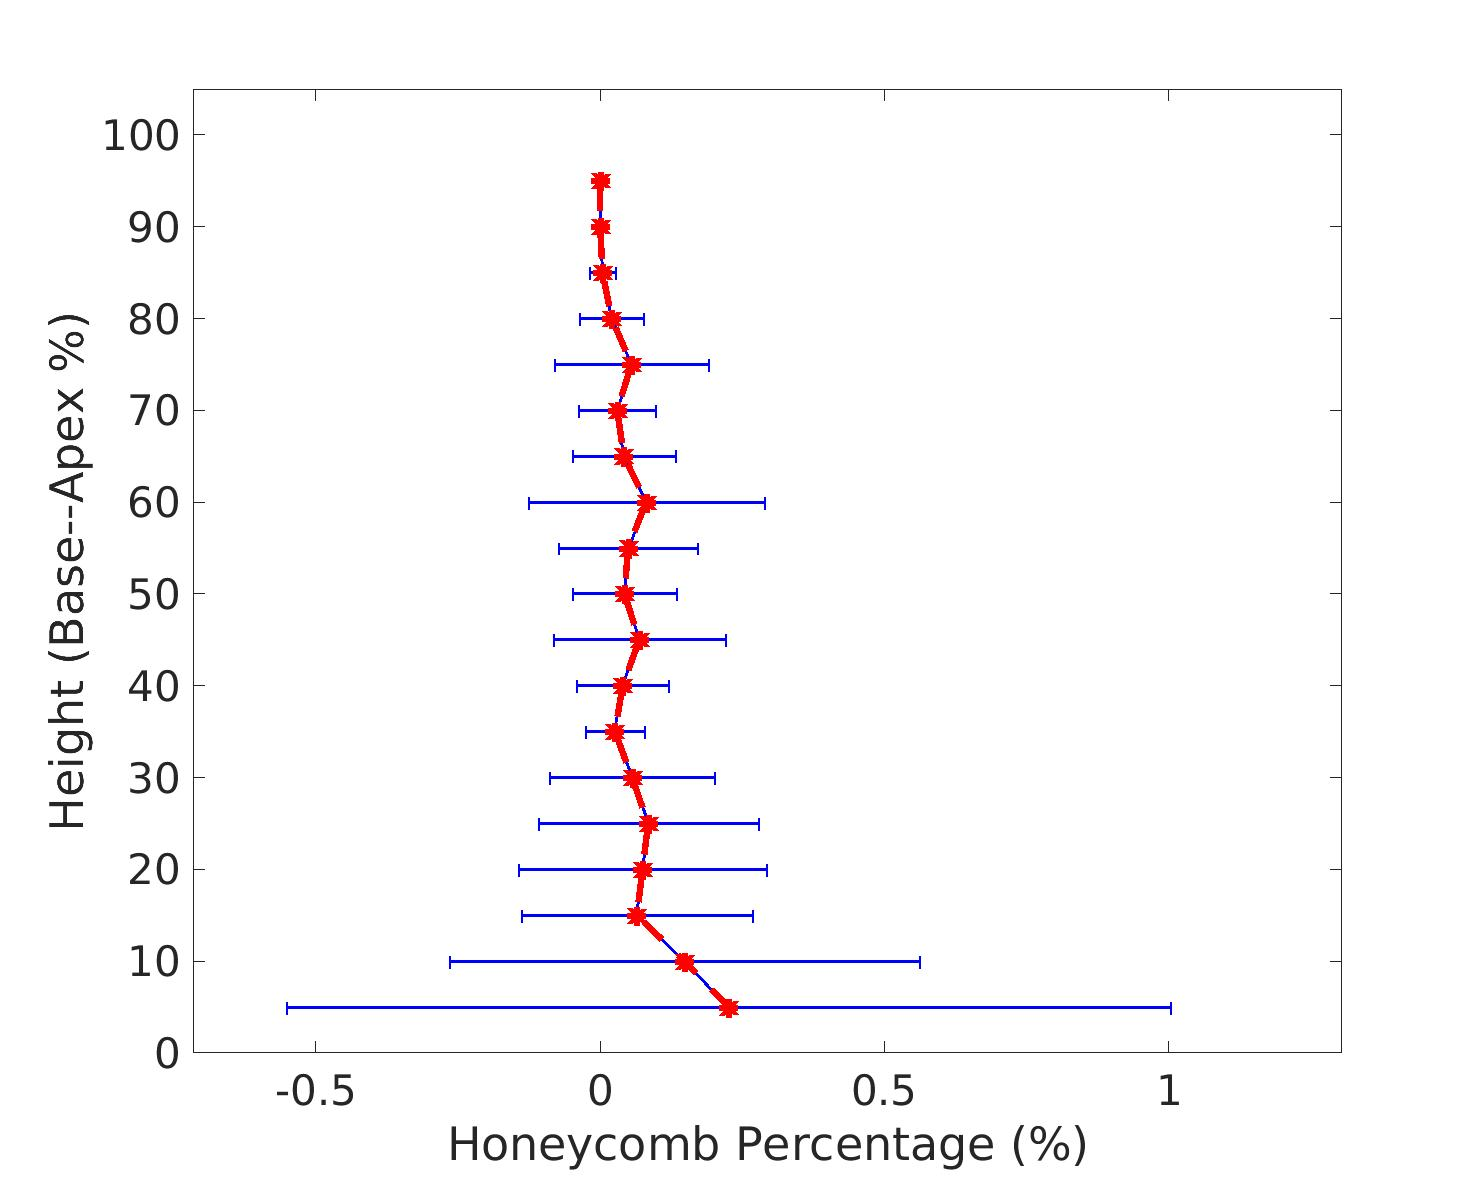
\includegraphics{QuantitativeAnalysis/Image/LeftLungHoneycombDiseaseAgainstHeight.jpg}} 
  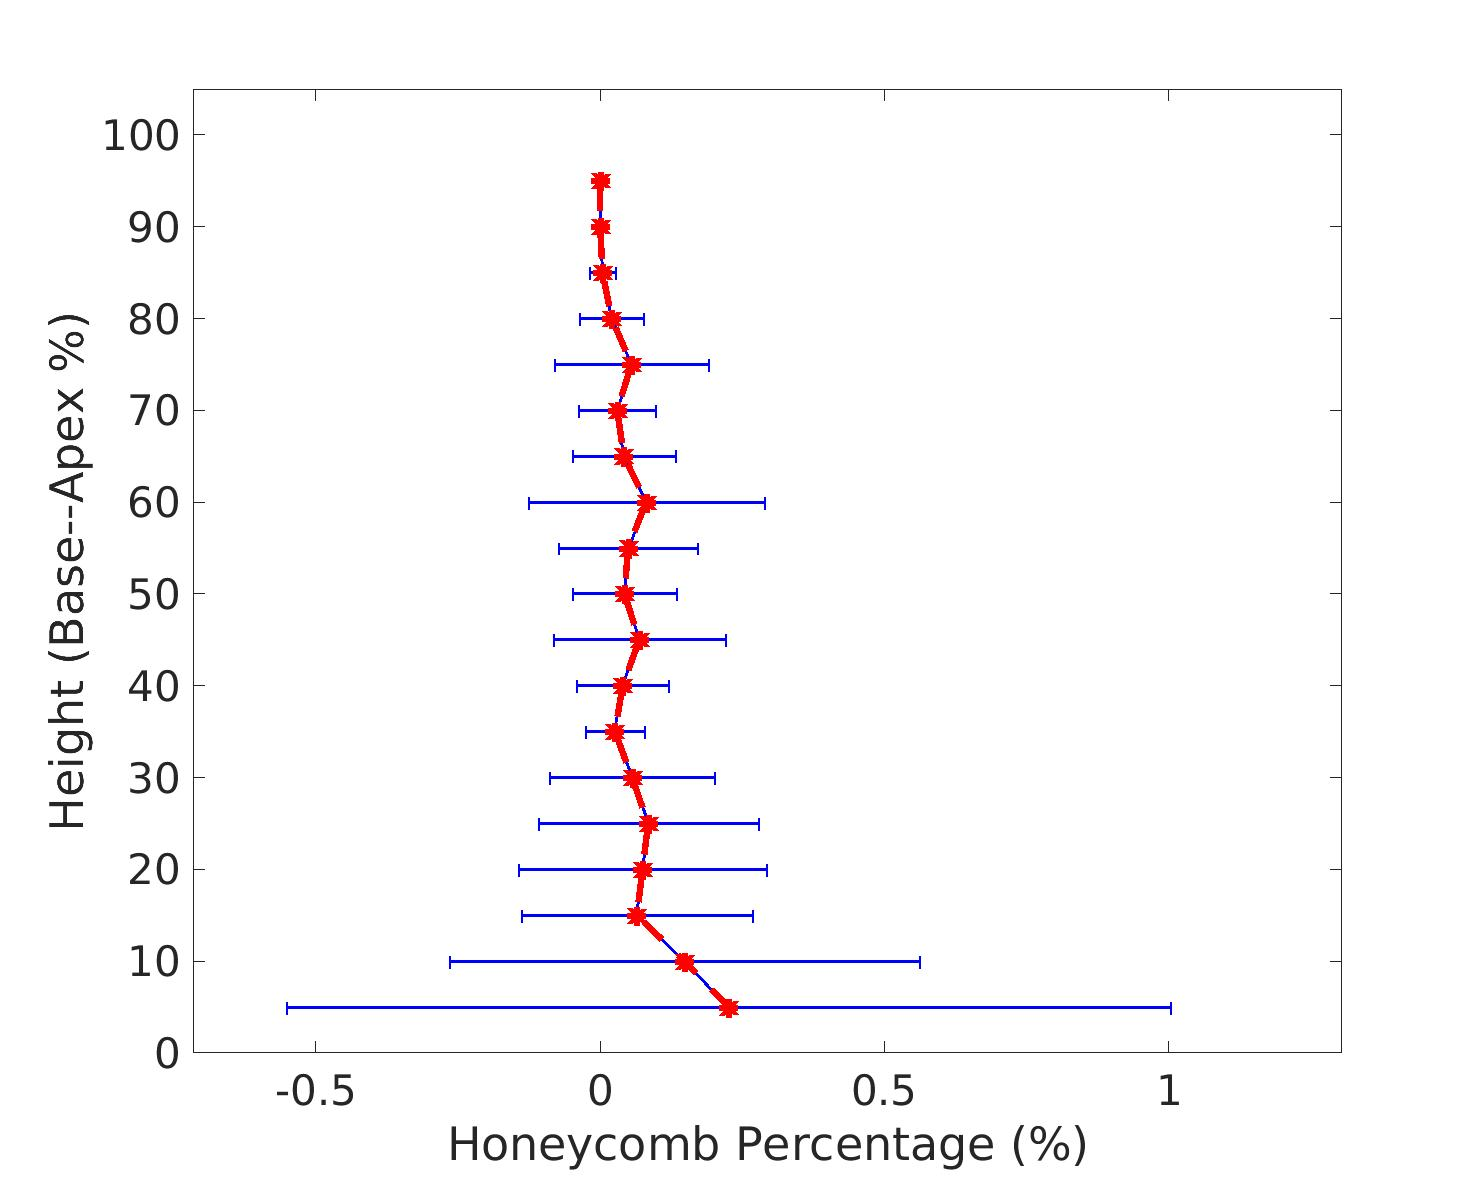
\includegraphics[width=\linewidth,trim={{.0\wd0} {.0\wd0} {.0\wd0} {.0\wd0}},clip]{QuantitativeAnalysis/Image/LeftLungHoneycombDiseaseAgainstHeight.jpg} %trim={<left> <lower> <right> <upper>}, set the cut scale
  \caption{}
  \label{fig:DiseaseAgainstHeight-e} 
\end{subfigure} 
\begin{subfigure}{.4\linewidth}% set image scale
  \sbox0{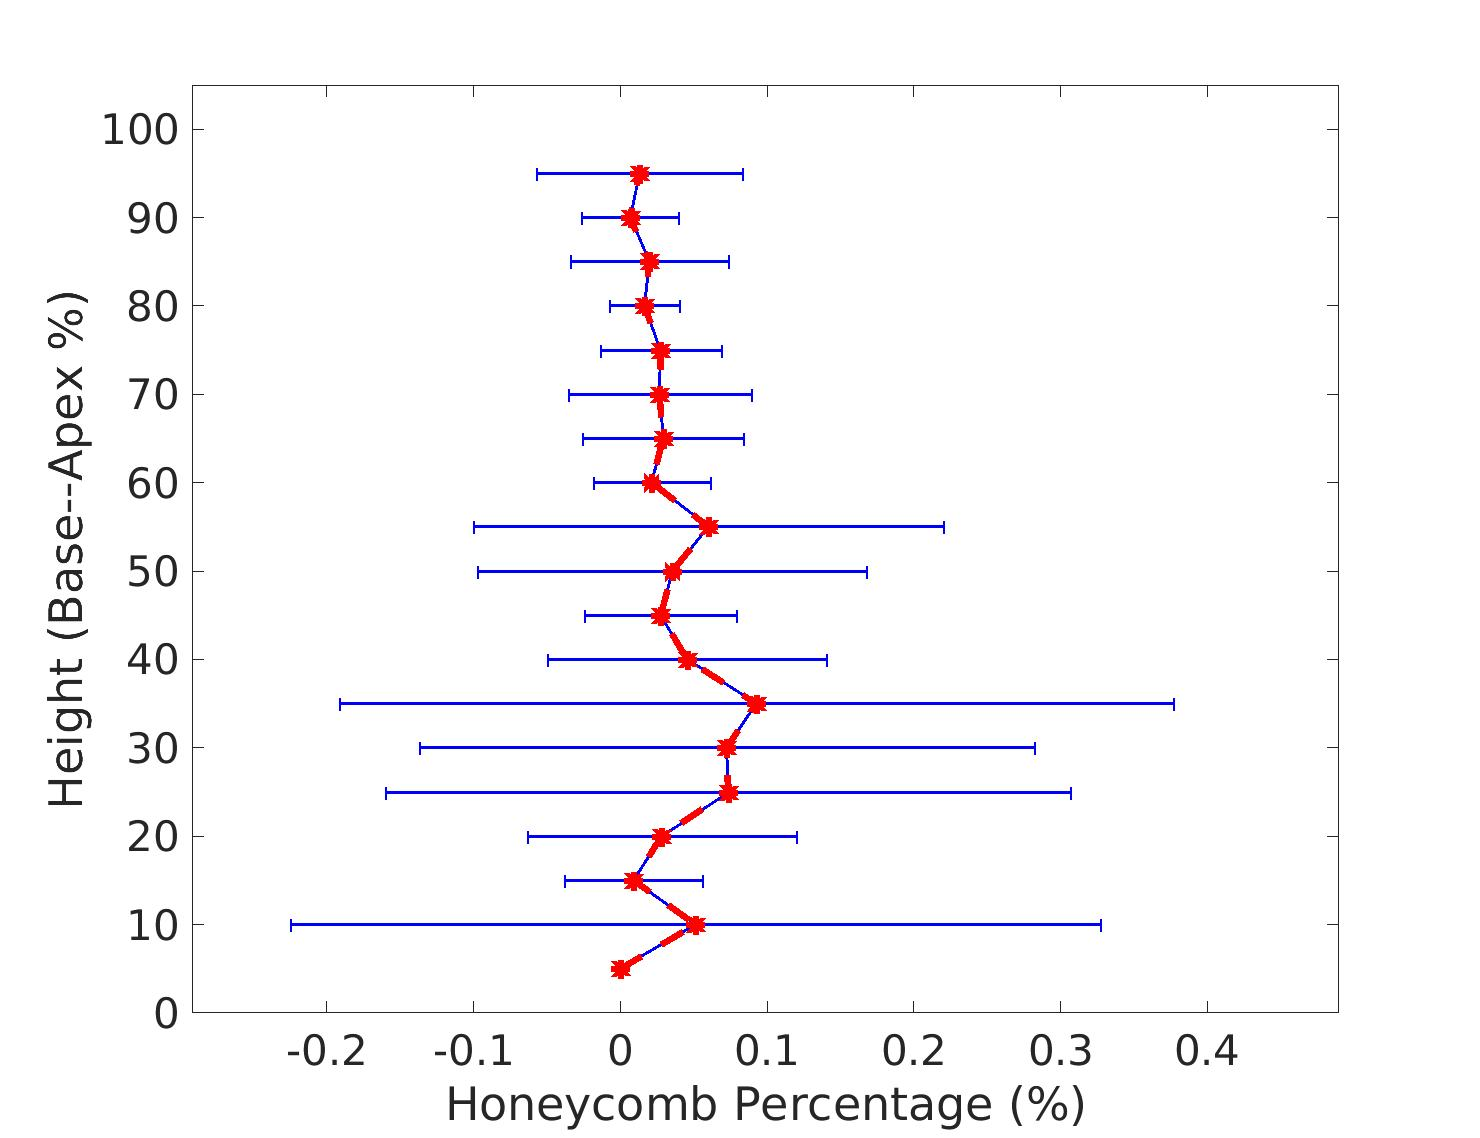
\includegraphics{QuantitativeAnalysis/Image/RightLungHoneycombDiseaseAgainstHeight.jpg}}
  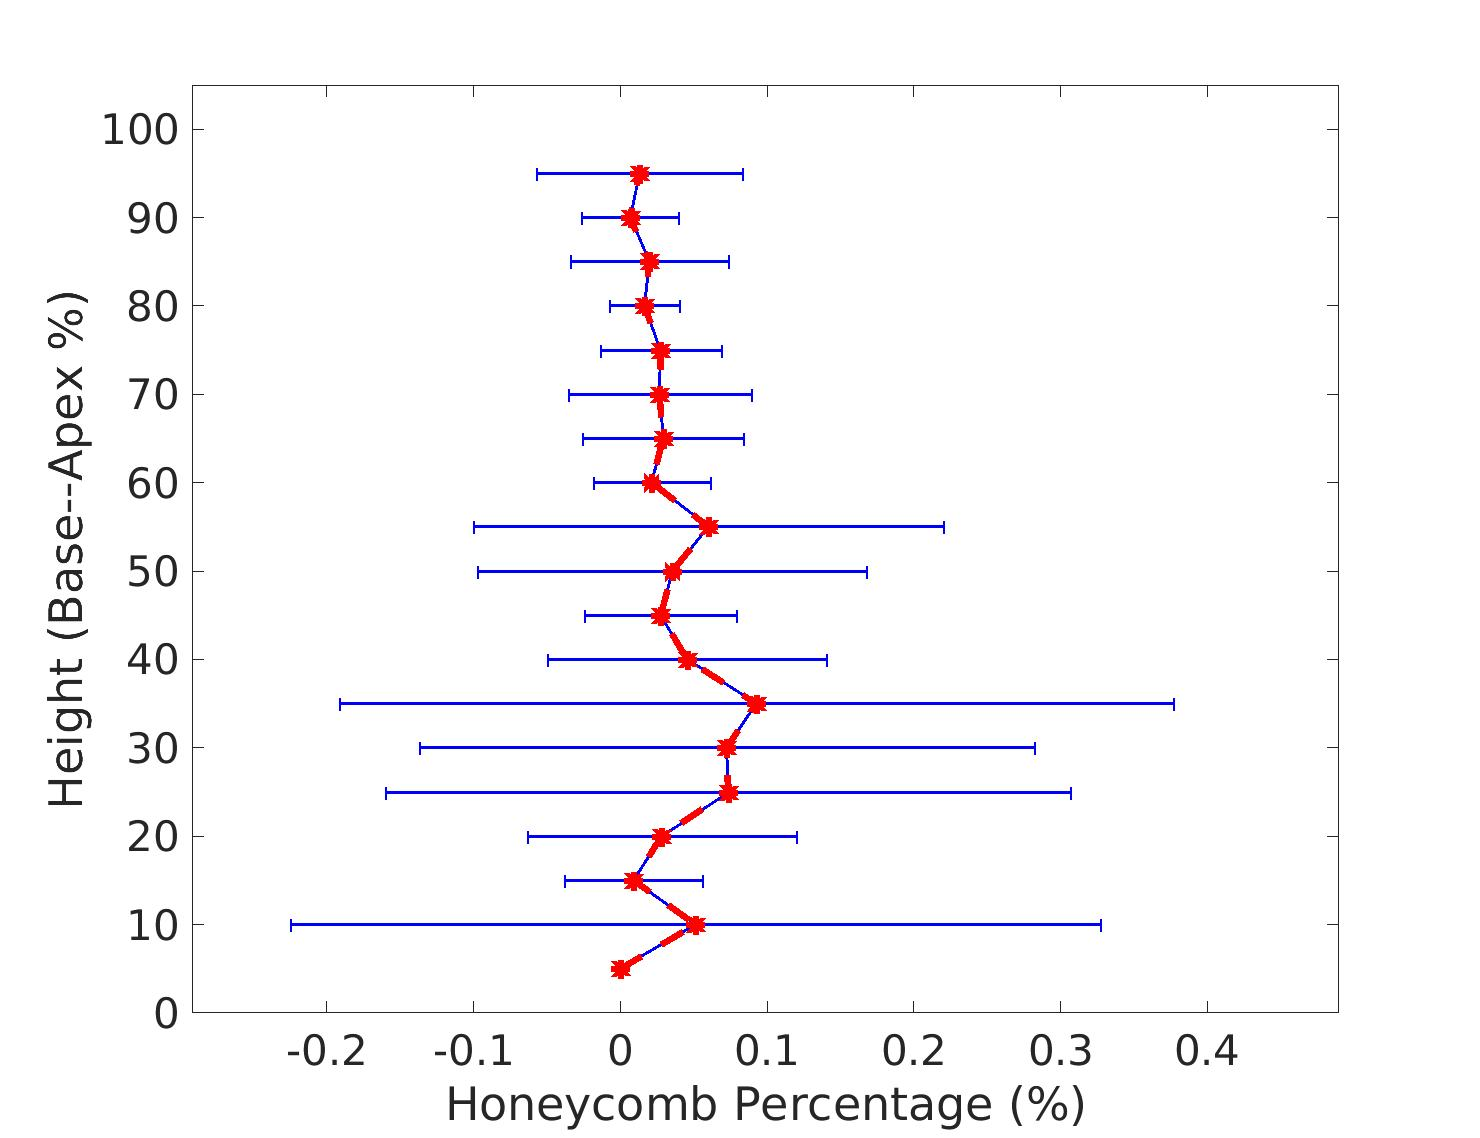
\includegraphics[width=\linewidth,trim={{.0\wd0} {.0\wd0} {.0\wd0} {.0\wd0}},clip]{QuantitativeAnalysis/Image/RightLungHoneycombDiseaseAgainstHeight.jpg}
  \caption{}
  \label{fig:DiseaseAgainstHeight-f}
\end{subfigure}
\begin{subfigure}{.4\linewidth}% set image scale
  \sbox0{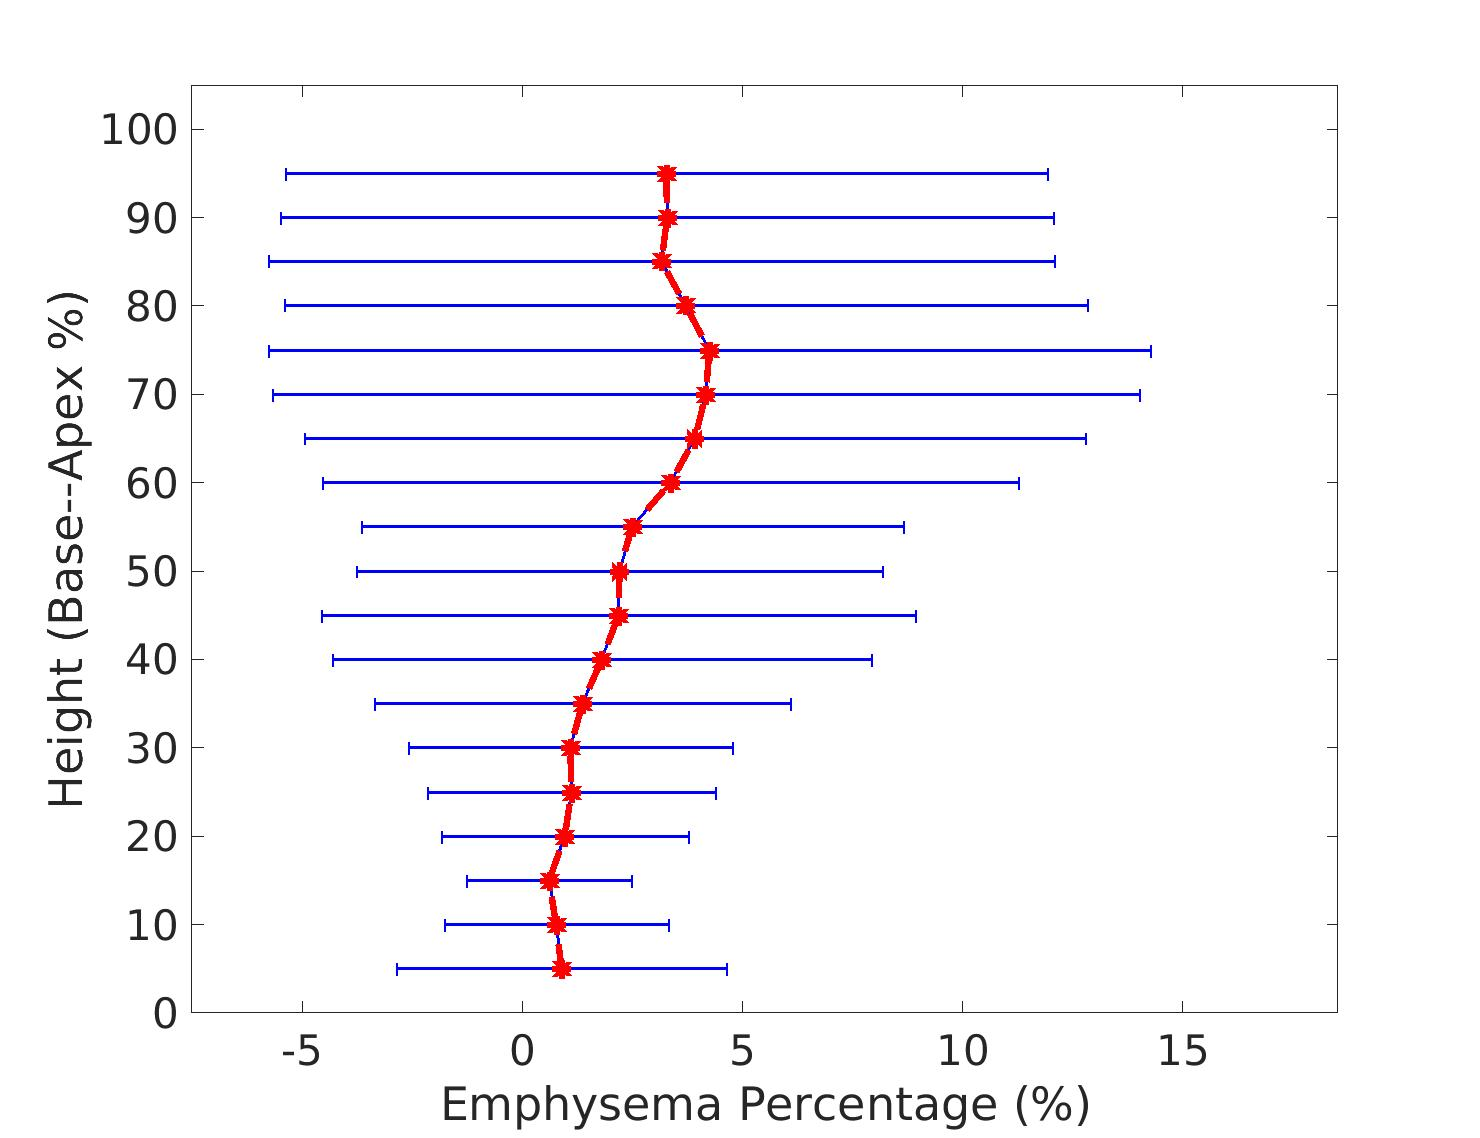
\includegraphics{QuantitativeAnalysis/Image/LeftLungEmphysemaDiseaseAgainstHeight.jpg}} 
  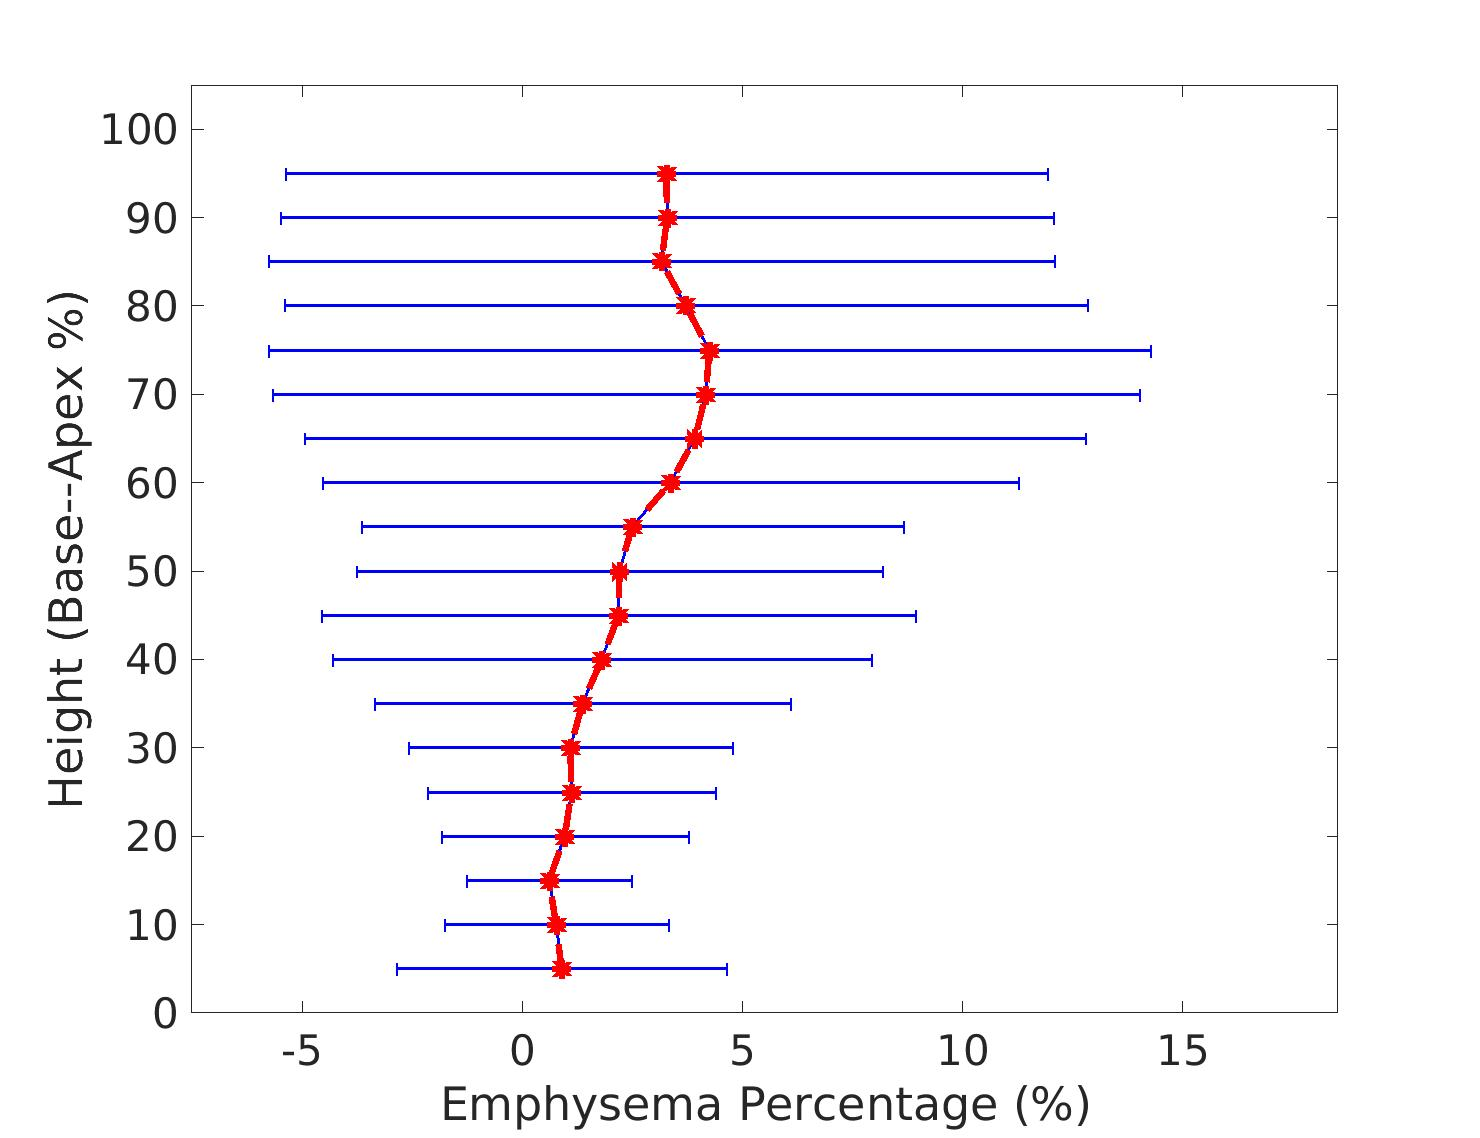
\includegraphics[width=\linewidth,trim={{.0\wd0} {.0\wd0} {.0\wd0} {.0\wd0}},clip]{QuantitativeAnalysis/Image/LeftLungEmphysemaDiseaseAgainstHeight.jpg} %trim={<left> <lower> <right> <upper>}, set the cut scale
  \caption{}
  \label{fig:DiseaseAgainstHeight-g} 
\end{subfigure} 
\begin{subfigure}{.4\linewidth}% set image scale
  \sbox0{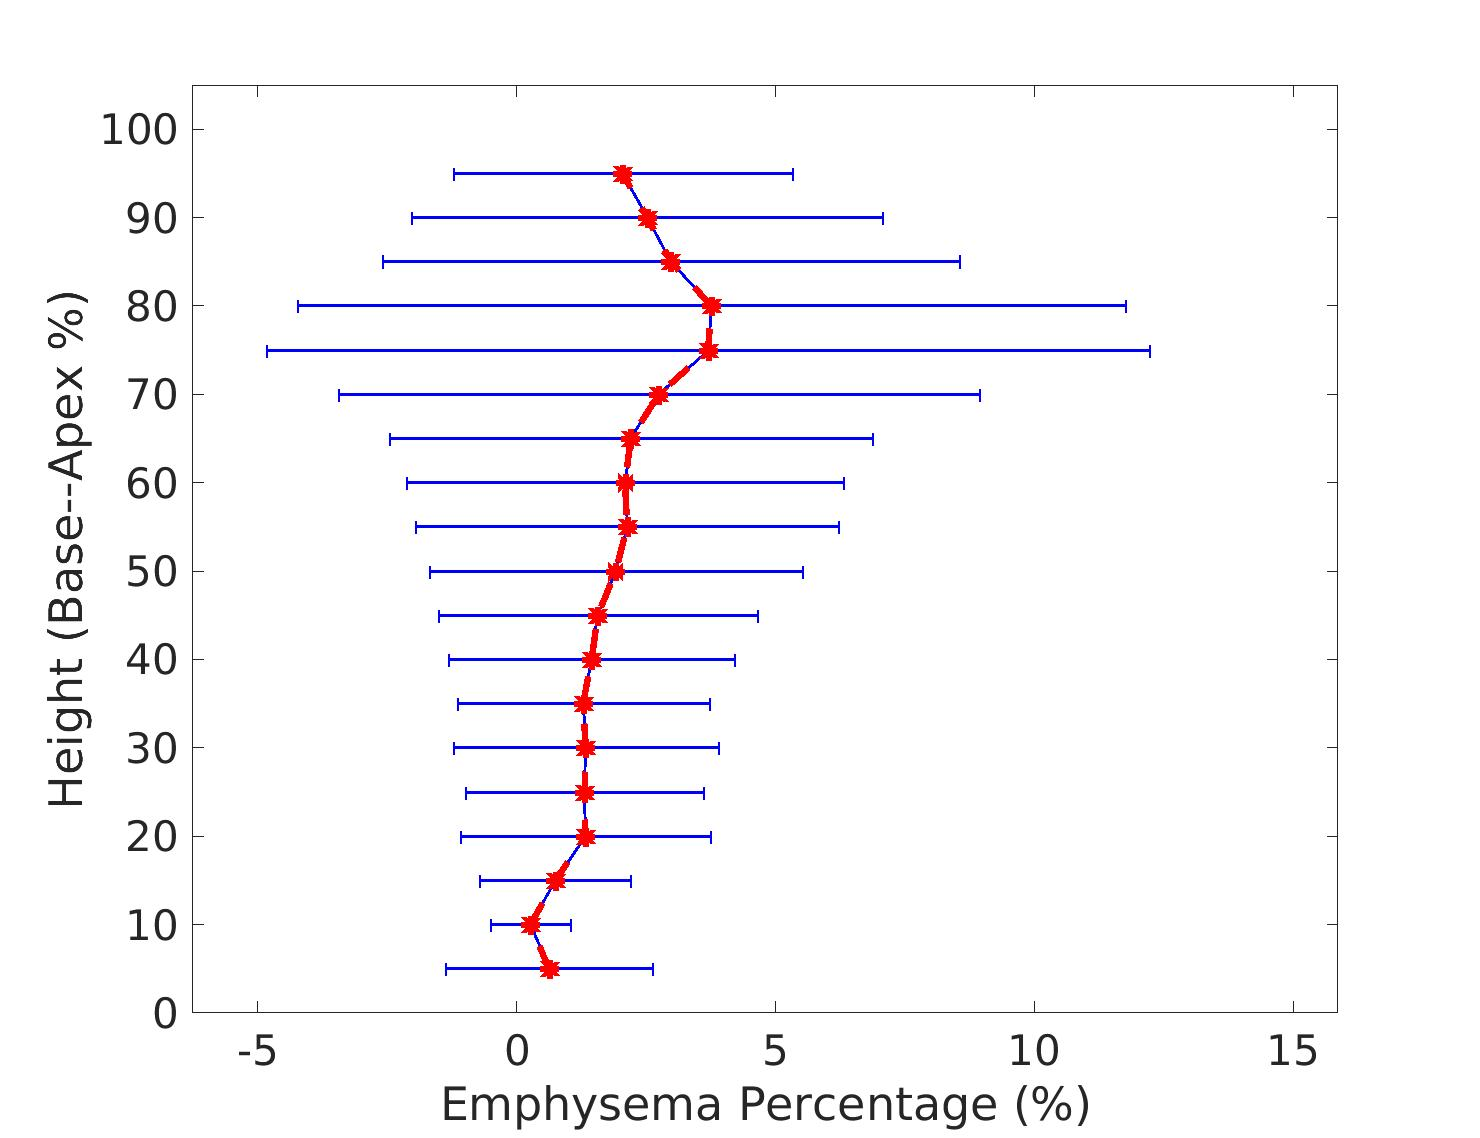
\includegraphics{QuantitativeAnalysis/Image/RightLungEmphysemaDiseaseAgainstHeight.jpg}}
  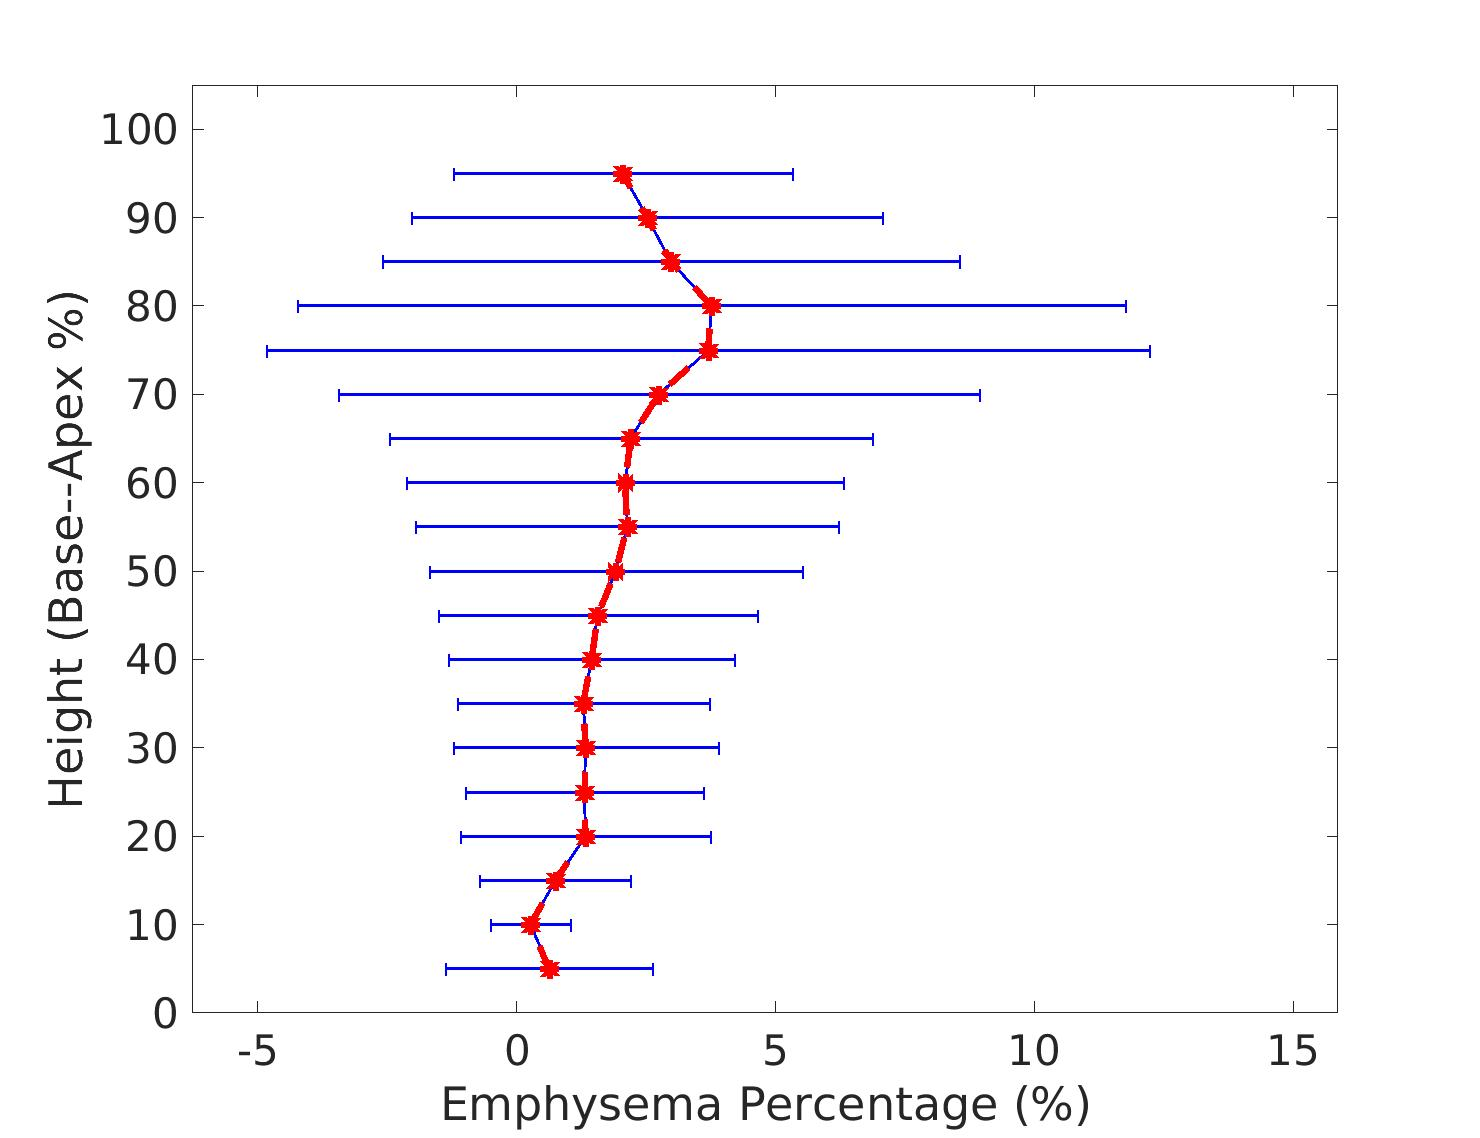
\includegraphics[width=\linewidth,trim={{.0\wd0} {.0\wd0} {.0\wd0} {.0\wd0}},clip]{QuantitativeAnalysis/Image/RightLungEmphysemaDiseaseAgainstHeight.jpg}
  \caption{}
  \label{fig:DiseaseAgainstHeight-h}
\end{subfigure}
\caption{Volume percentage of each disease CT pattern plotted against lung height (dorsoventral axis) in IPF left and right lungs. The percentage was calculated as the average within 5\% of the lung height from the base to apex. The red line represents the average value at each position across all patients, and the blue line shows the standard deviation. (a) (b) shows ground-glass distribution. (c) (d) shows reticular distribution. (e) (f) shows honeycomb distribution. (g) (h) show emphysema distribution.}
\label{fig:DiseaseAgainstHeight}
\end{figure}

2. Lobar distribution: In order to analyze the lobar distribution of disease, the volume percentage of each disease CT pattern located in each lobe was calculated.

Figure \ref{fig:LobarRegionDiseaseDistributionAverage} shows the volume percentage of four characteristic CT patterns: ground-glass, reticular, honeycomb and emphysema in the five lobes (left upper, left lower, right upper, right middle, right lower). Fibrosis area locates predominantly in lower lobes (72\%, 58\%, 65\% for honeycomb, reticular, ground-glass). For reticular pattern, the percentage in the middle lobe is lower than the percentage of other lobes, which means reticular pattern rarely locates in the middle part of the lung. As for emphysema lesions, it commonly presents in the upper lobes (73\%) and may also appear in the middle lobe as the disease progresses.

\begin{figure}[htbp] 
\centering
\begin{subfigure}{.46\linewidth}% set image scale
  \sbox0{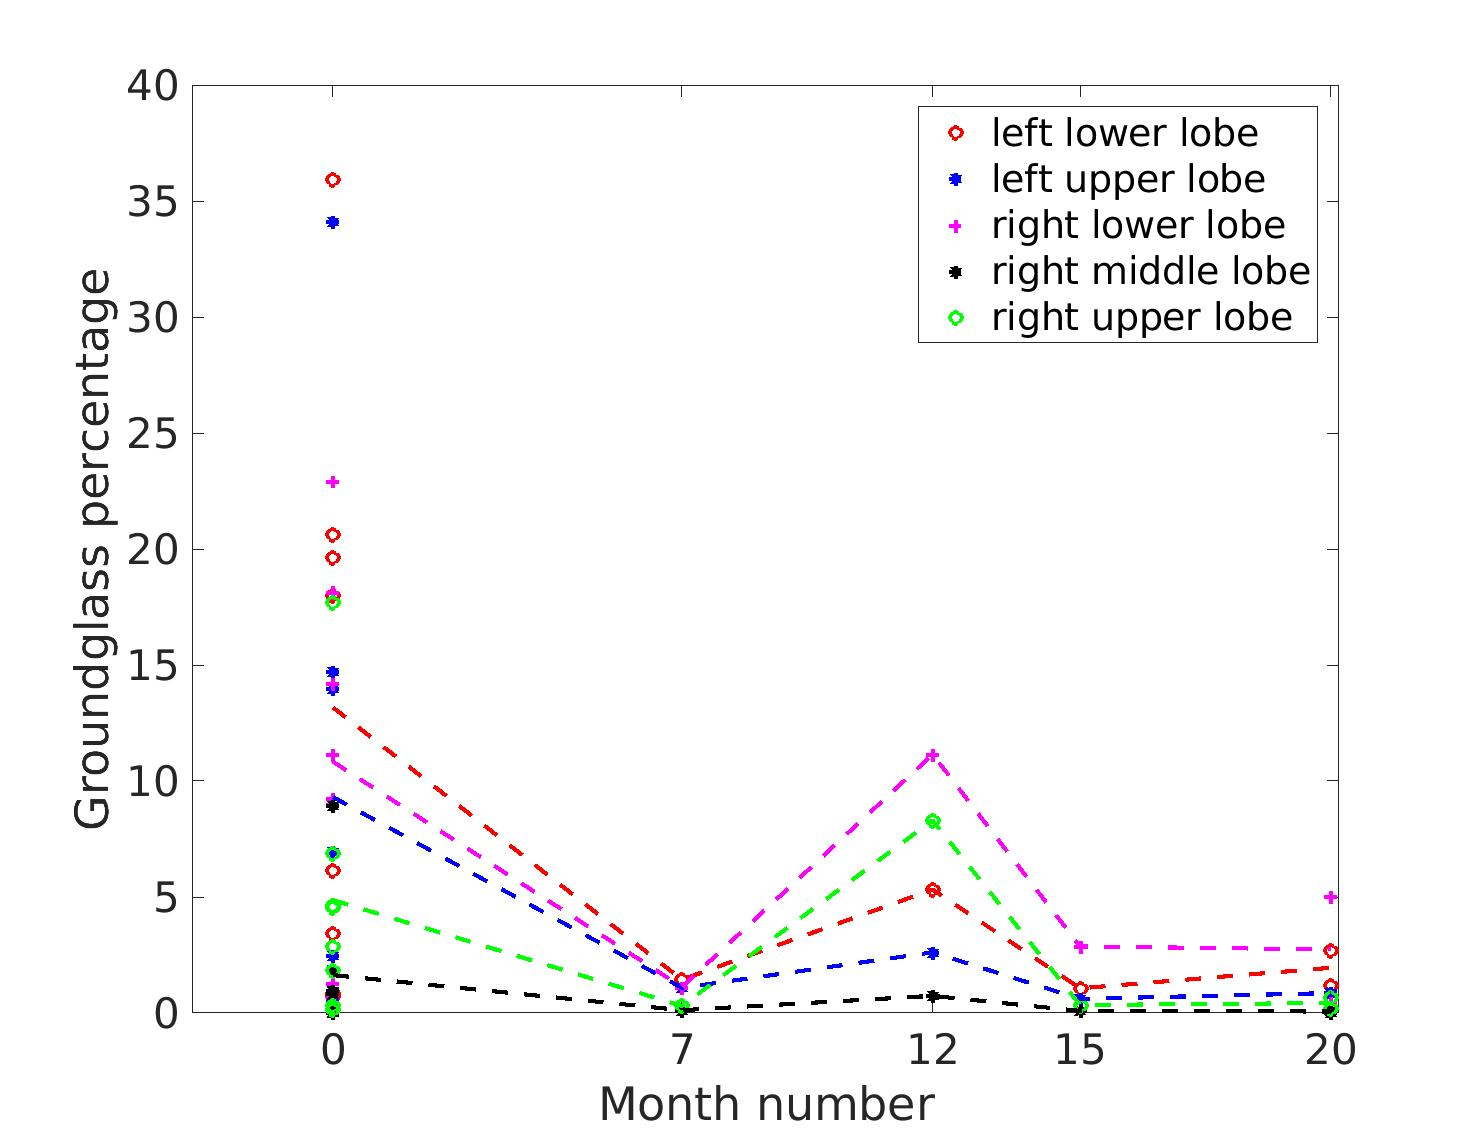
\includegraphics{QuantitativeAnalysis/Image/GroundglassLobarRegionDiseaseDistributionAverage.jpg}} 
  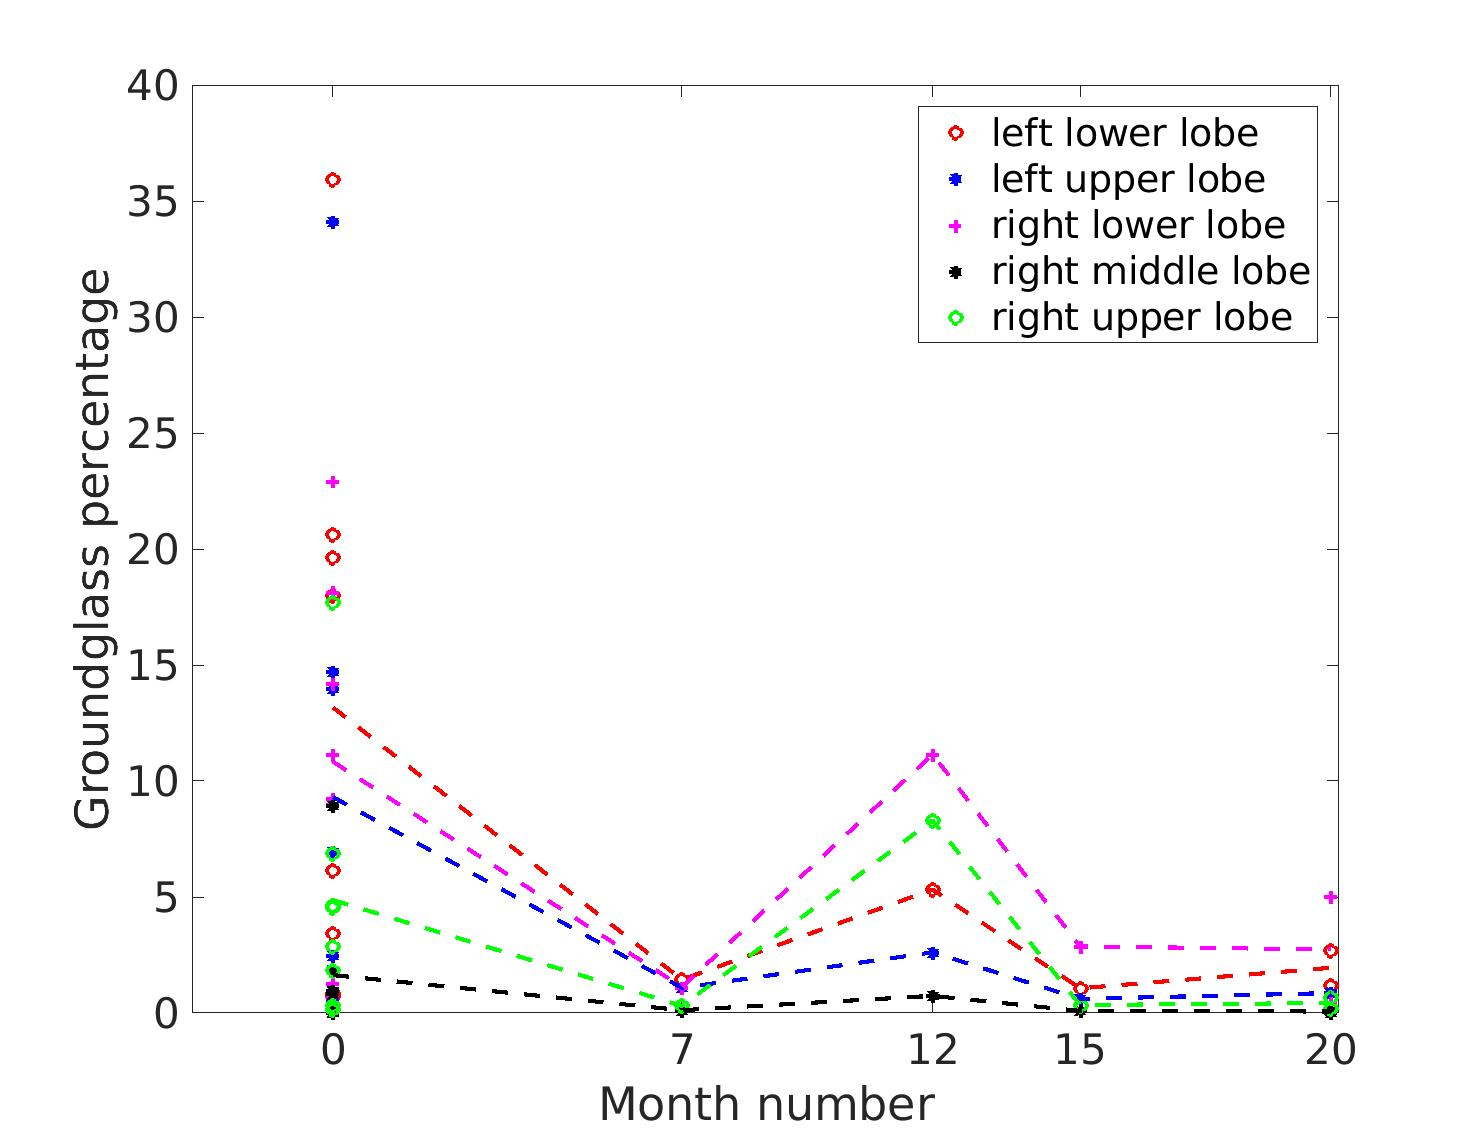
\includegraphics[width=\linewidth,trim={{.0\wd0} {.0\wd0} {.0\wd0} {.0\wd0}},clip]{QuantitativeAnalysis/Image/GroundglassLobarRegionDiseaseDistributionAverage.jpg} %trim={<left> <lower> <right> <upper>}, set the cut scale
  \caption{}
  \label{fig:LobarRegionDiseaseDistributionAverage-a} 
\end{subfigure} 
\hspace{.3in}
\begin{subfigure}{.46\linewidth}% set image scale
  \sbox0{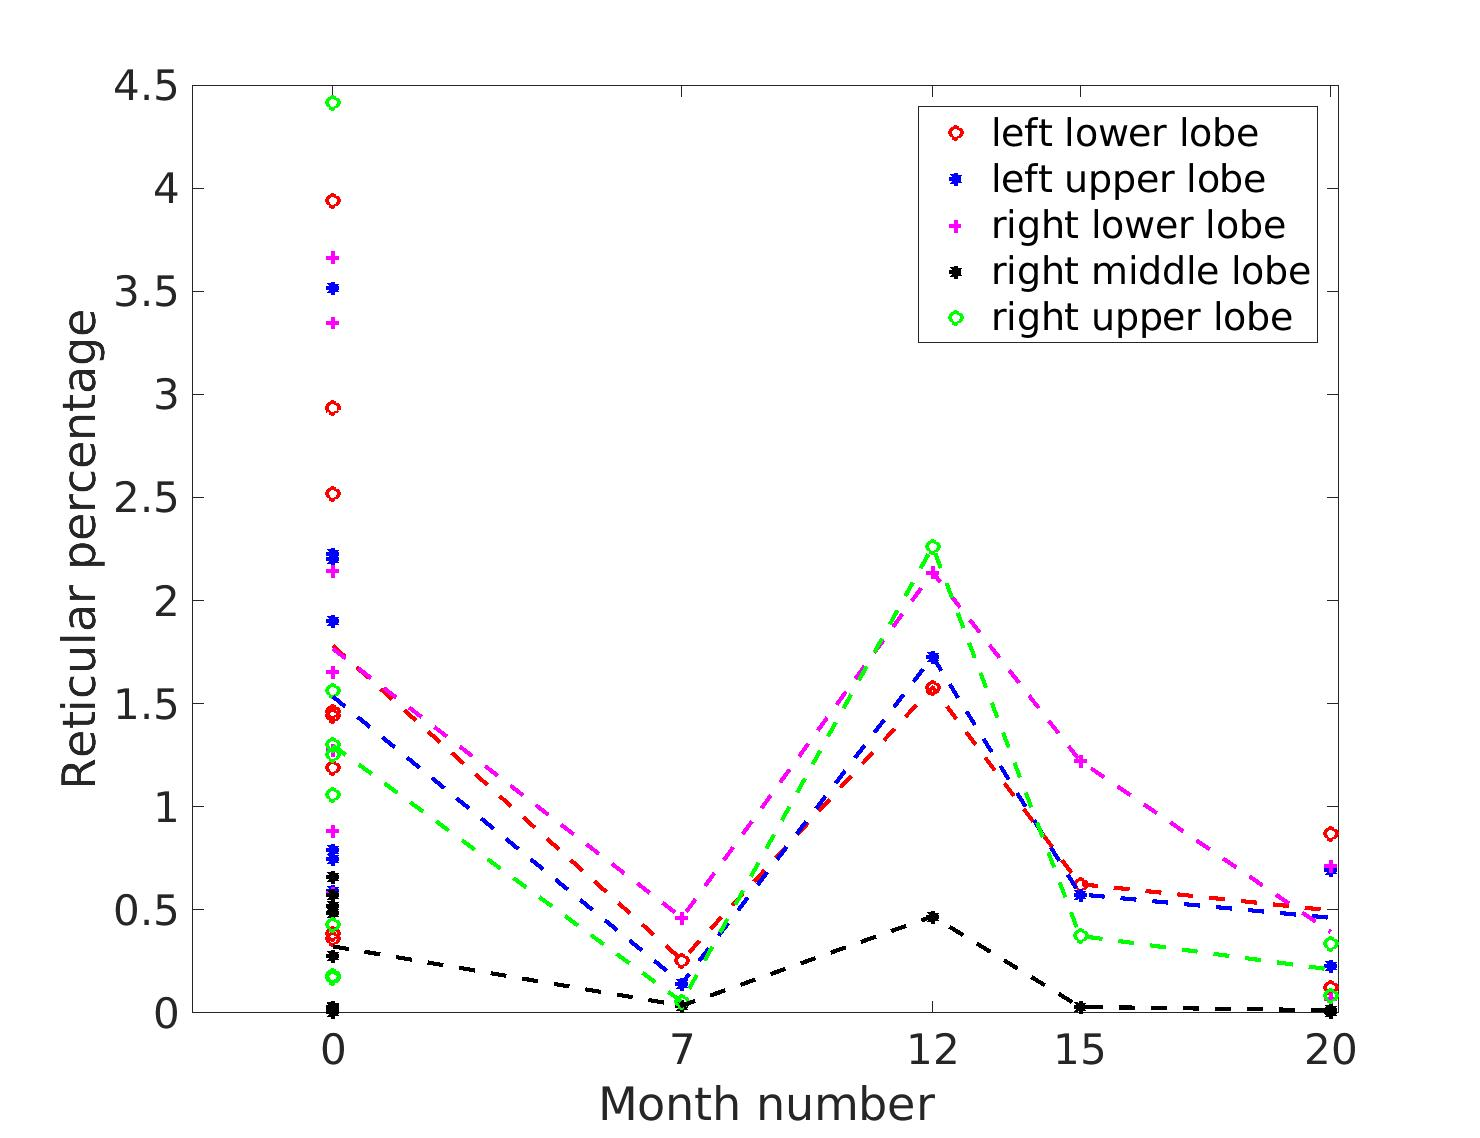
\includegraphics{QuantitativeAnalysis/Image/ReticularLobarRegionDiseaseDistributionAverage.jpg}}
  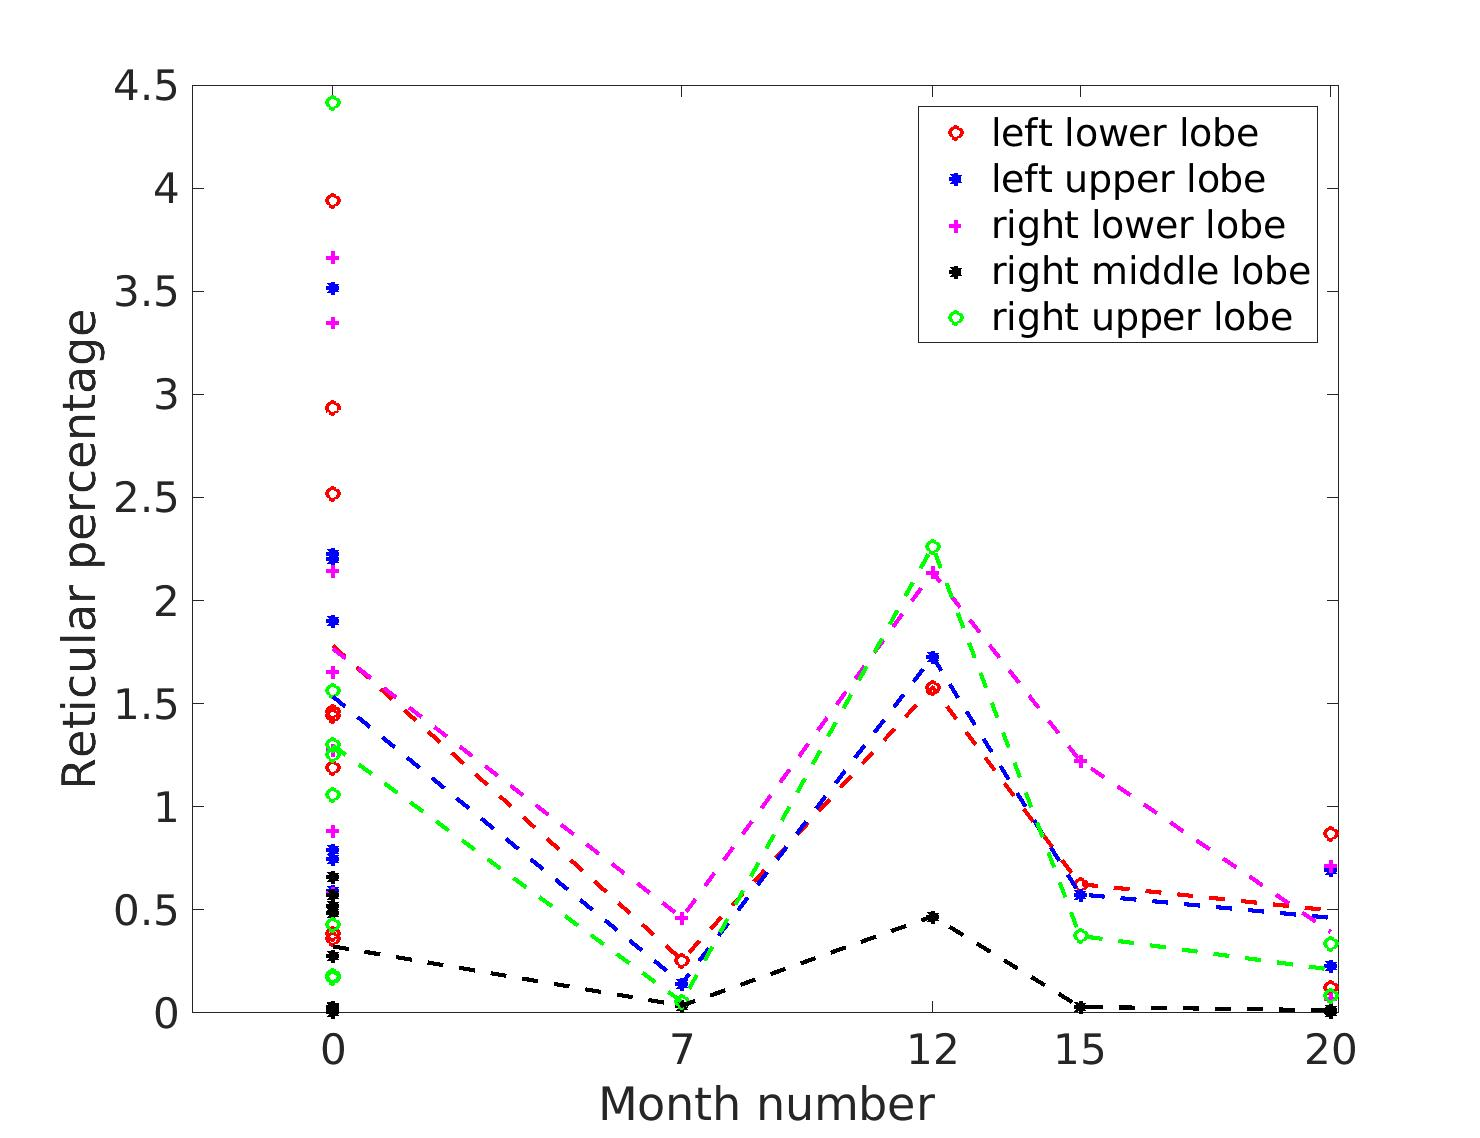
\includegraphics[width=\linewidth,trim={{.0\wd0} {.0\wd0} {.0\wd0} {.0\wd0}},clip]{QuantitativeAnalysis/Image/ReticularLobarRegionDiseaseDistributionAverage.jpg}
  \caption{}
  \label{fig:LobarRegionDiseaseDistributionAverage-b}
\end{subfigure}
\begin{subfigure}{.46\linewidth}% set image scale
  \sbox0{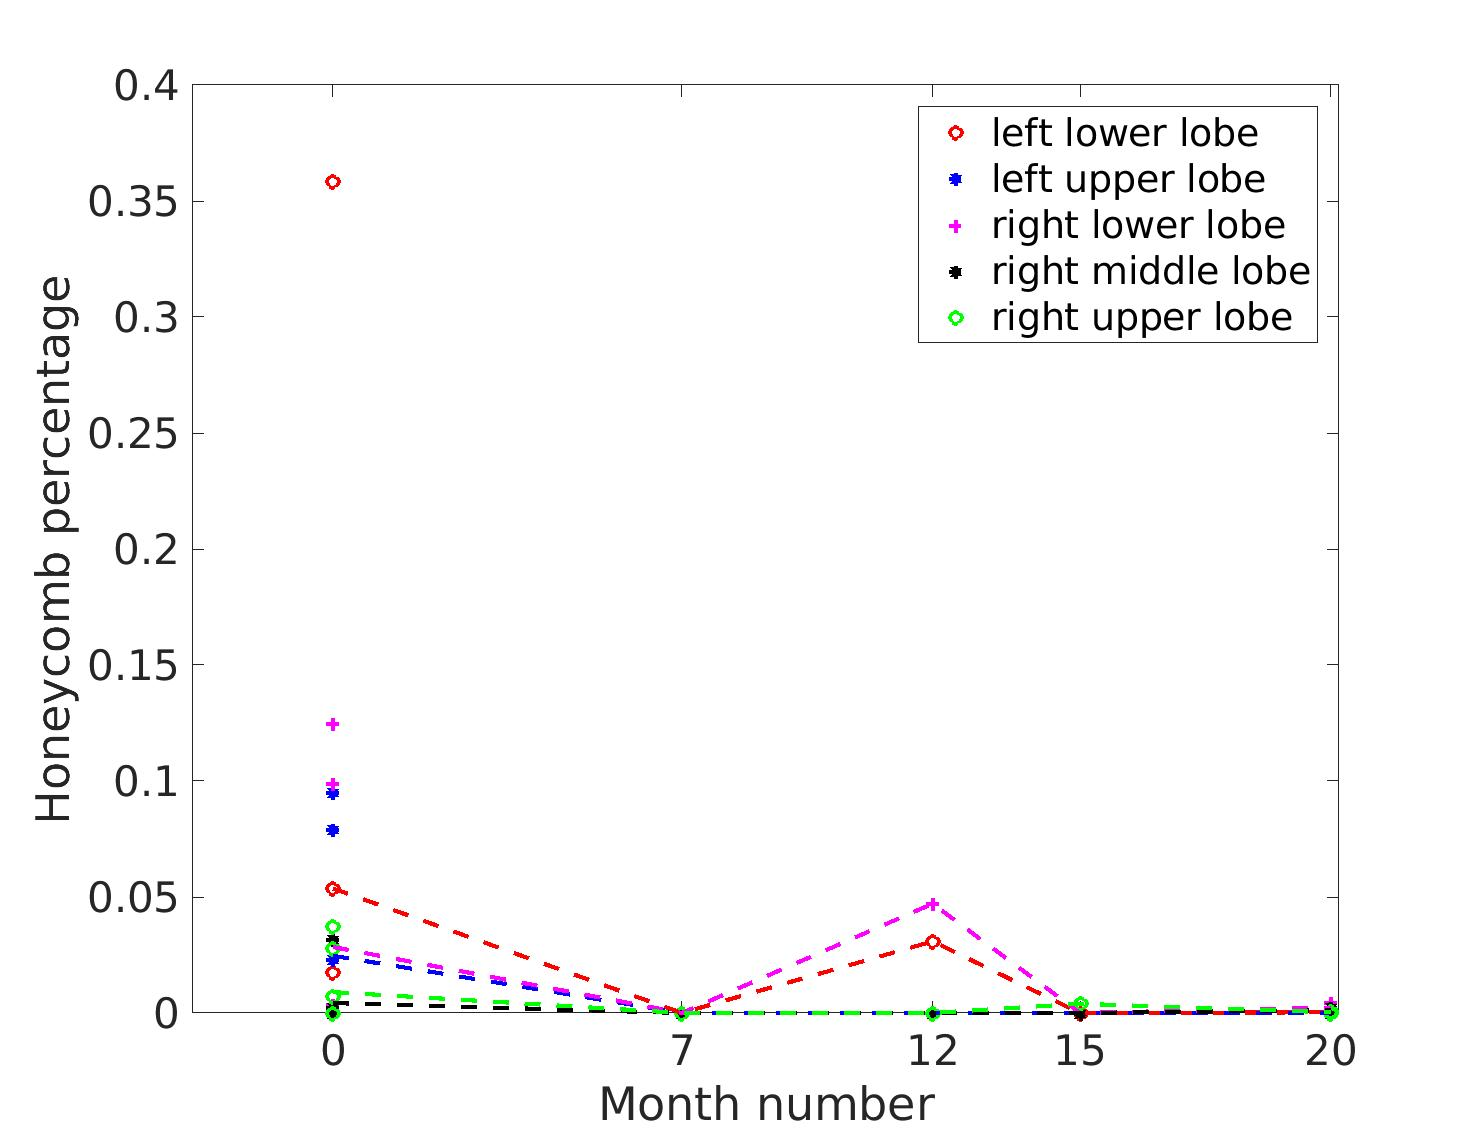
\includegraphics{QuantitativeAnalysis/Image/HoneycombLobarRegionDiseaseDistributionAverage.jpg}} 
  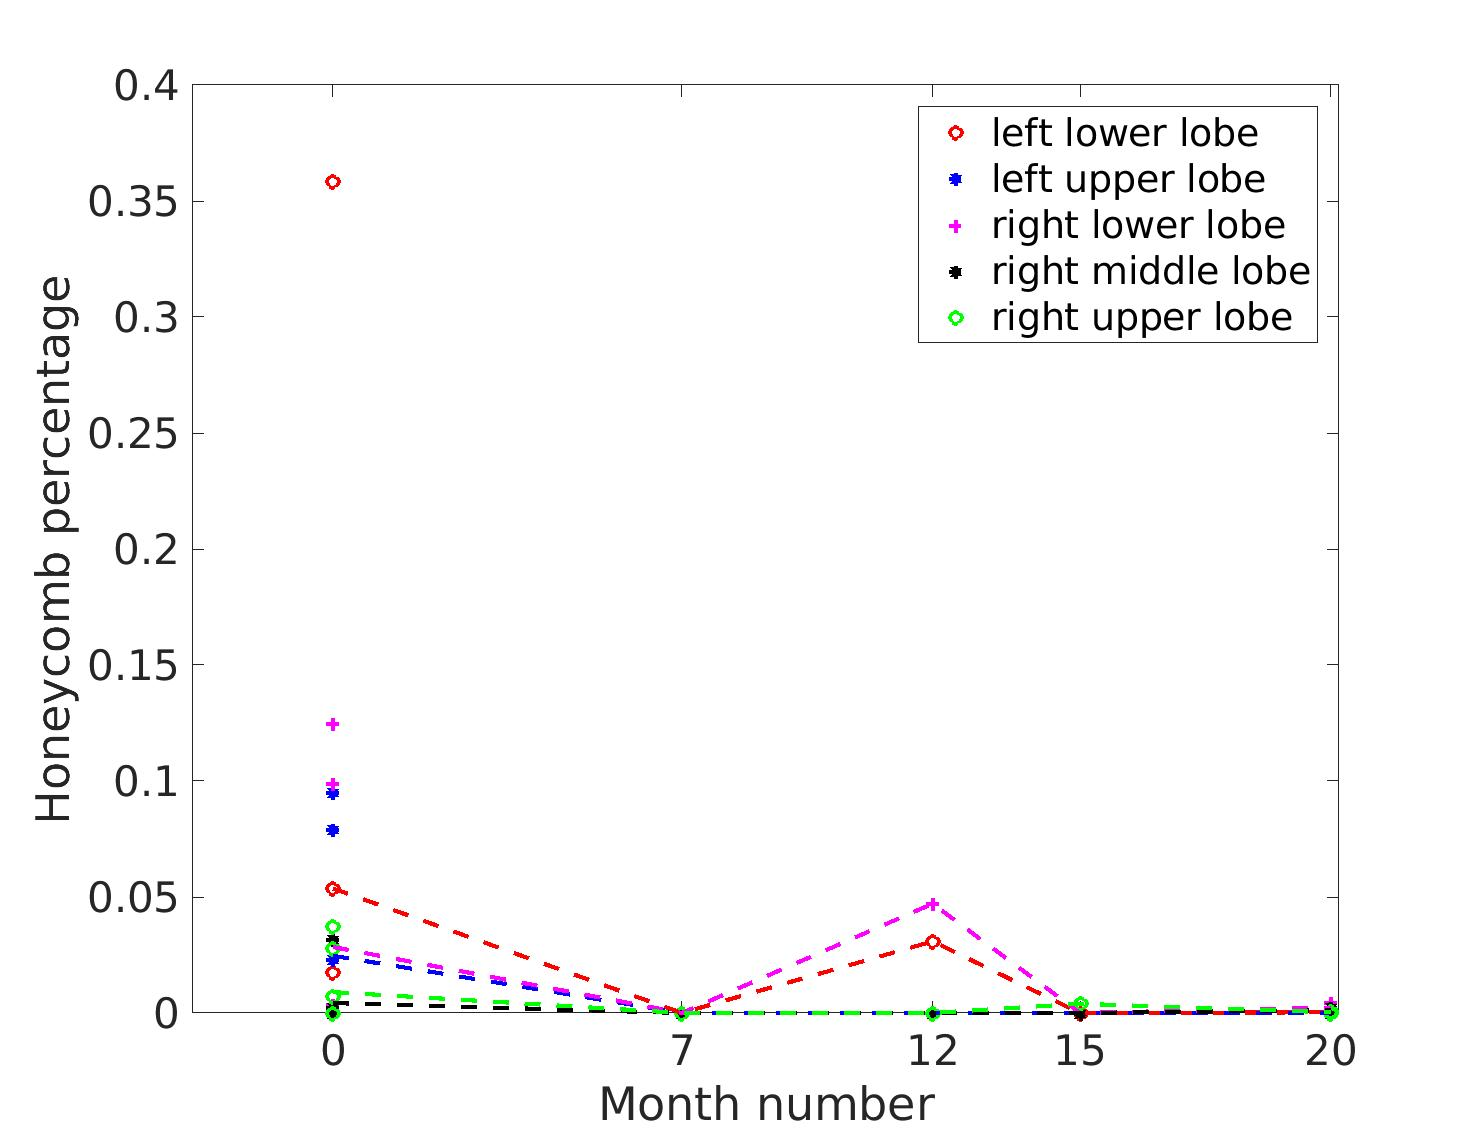
\includegraphics[width=\linewidth,trim={{.0\wd0} {.0\wd0} {.0\wd0} {.0\wd0}},clip]{QuantitativeAnalysis/Image/HoneycombLobarRegionDiseaseDistributionAverage.jpg} %trim={<left> <lower> <right> <upper>}, set the cut scale
  \caption{}
  \label{fig:LobarRegionDiseaseDistributionAverage-c} 
\end{subfigure} 
\hspace{.3in}
\begin{subfigure}{.46\linewidth}% set image scale
  \sbox0{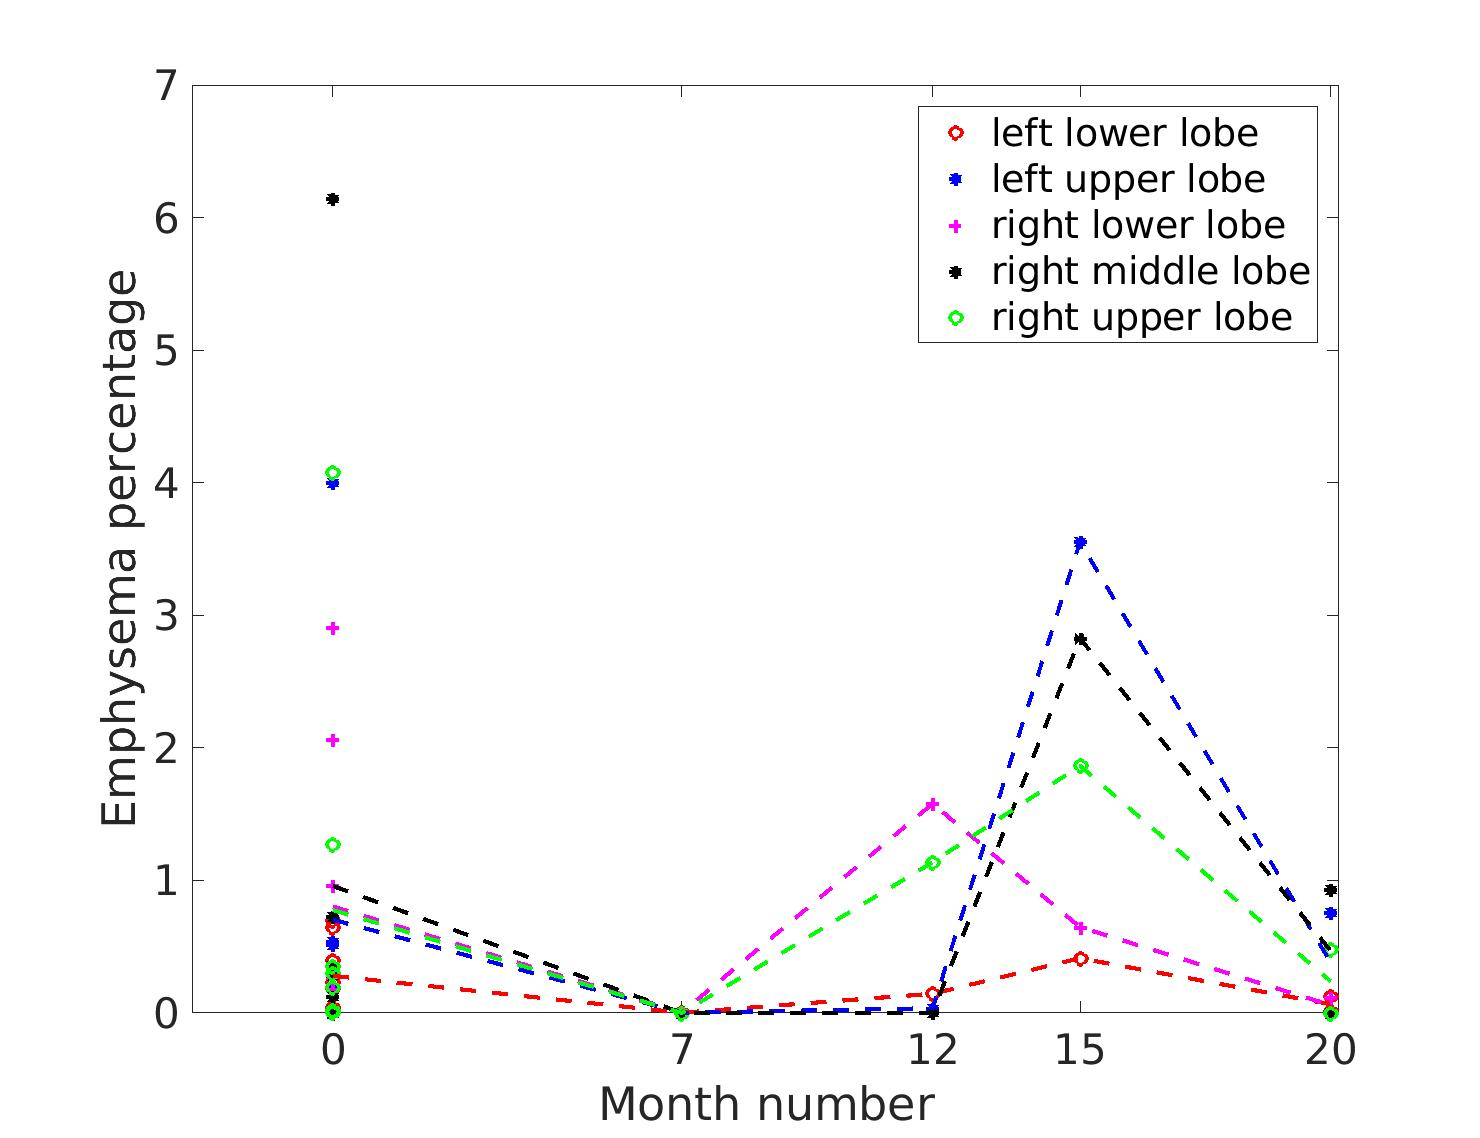
\includegraphics{QuantitativeAnalysis/Image/EmphysemaLobarRegionDiseaseDistributionAverage.jpg}}
  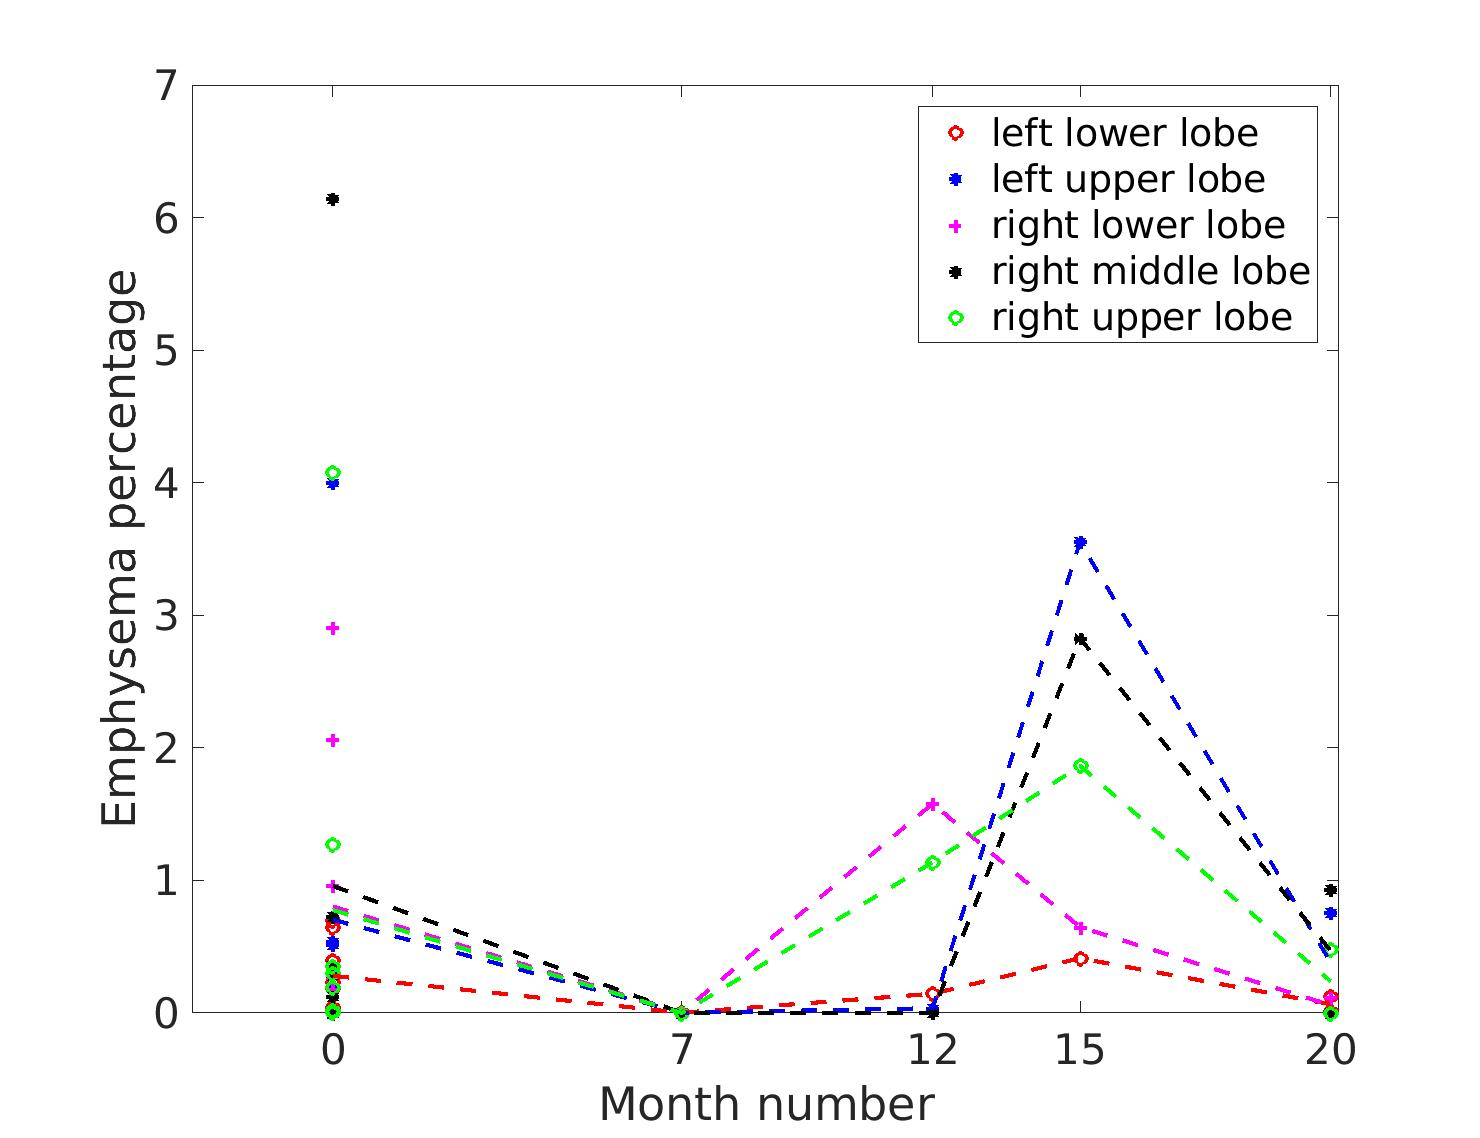
\includegraphics[width=\linewidth,trim={{.0\wd0} {.0\wd0} {.0\wd0} {.0\wd0}},clip]{QuantitativeAnalysis/Image/EmphysemaLobarRegionDiseaseDistributionAverage.jpg}
  \caption{}
  \label{fig:LobarRegionDiseaseDistributionAverage-d}
\end{subfigure}
\caption{Lobar distribution of disease CT patterns. The x-axis shows the time interval (in months) of scan time for each patient, with x=0 representing the first scan for this patient. Each point represents the volume percentage of one CT pattern for one lobe. The dotted line represents the average value aross all subjects for each time point. (a) Ground-glass lobar distribution. (b) Reticular lobar distribution. (c) Honeycomb lobar distribution. (d) Emphysema lobar distribution.}
\label{fig:LobarRegionDiseaseDistributionAverage}
\end{figure}

3. Subplerual to internal: The distance from the abnormalities to the boundary of the lung and to the center of the lung were measured to analyze the peripheral performance of disease. To be specific, the center location of each connected cluster of disease area was firstly extracted, and the subpleural to internal percentage $R_{subpleural}$ of each connected cluster, which described how far was the conncected cluster from the lung surface, was then calculated as the diagram shown in Figure \ref{fig:SubpleuralMethod}

\begin{figure}[H]
  \centering 
  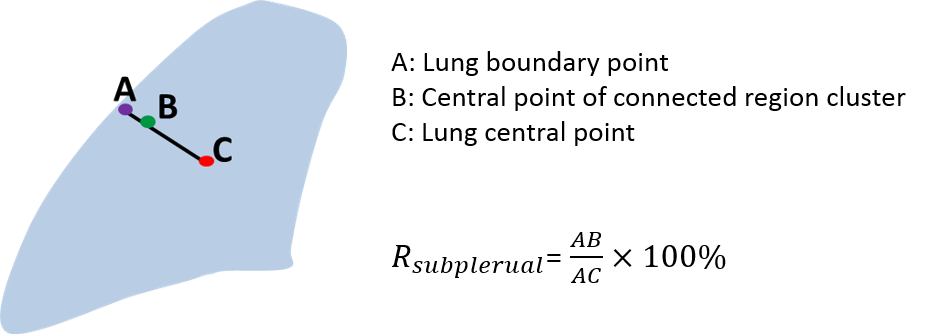
\includegraphics[height=1.8in]{QuantitativeAnalysis/Image/SubplesrualMethod.png}
  \caption{Diagram of subpleural-to-internal percentage measurement.}
  \label{fig:SubpleuralMethod}
\end{figure}
%
%\begin{equation}
%R_{subpleural} = \frac{AB}{AC} \times 100
%\end{equation}

Figure \ref{fig:DiseaseSubpleuralPercent} plots the subpleural-to-internal percentage of each connected cluster of three CT patterns: ground-glass, reticular and honeycomb. The result shows that the subpleural-to-internal percentage of most connected disease clusters are under 20\% for both left and right lungs, which quantitatively demonstrated that IPF disease are usually peripheral performance and mainly distributes surrounding the surface of the lung.

\begin{figure}[htbp] 
\centering
\begin{subfigure}{.5\linewidth}% set image scale
  \sbox0{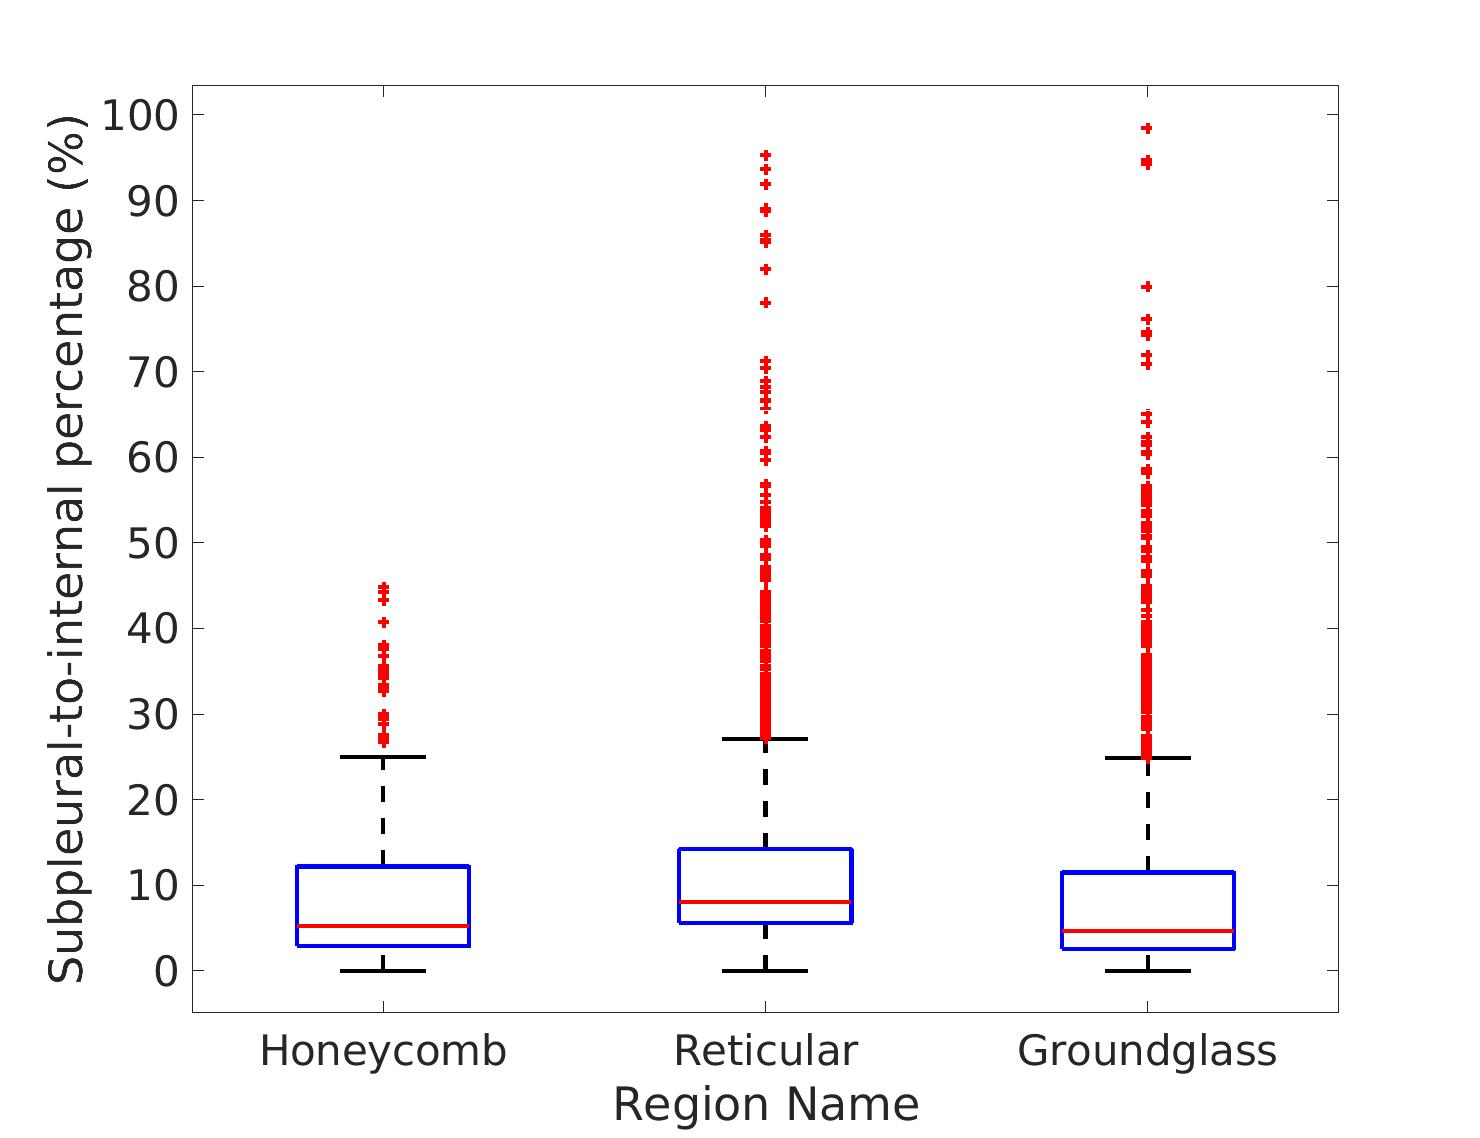
\includegraphics{QuantitativeAnalysis/Image/LeftLungDiseaseSubpleuralPercent.jpg}} 
  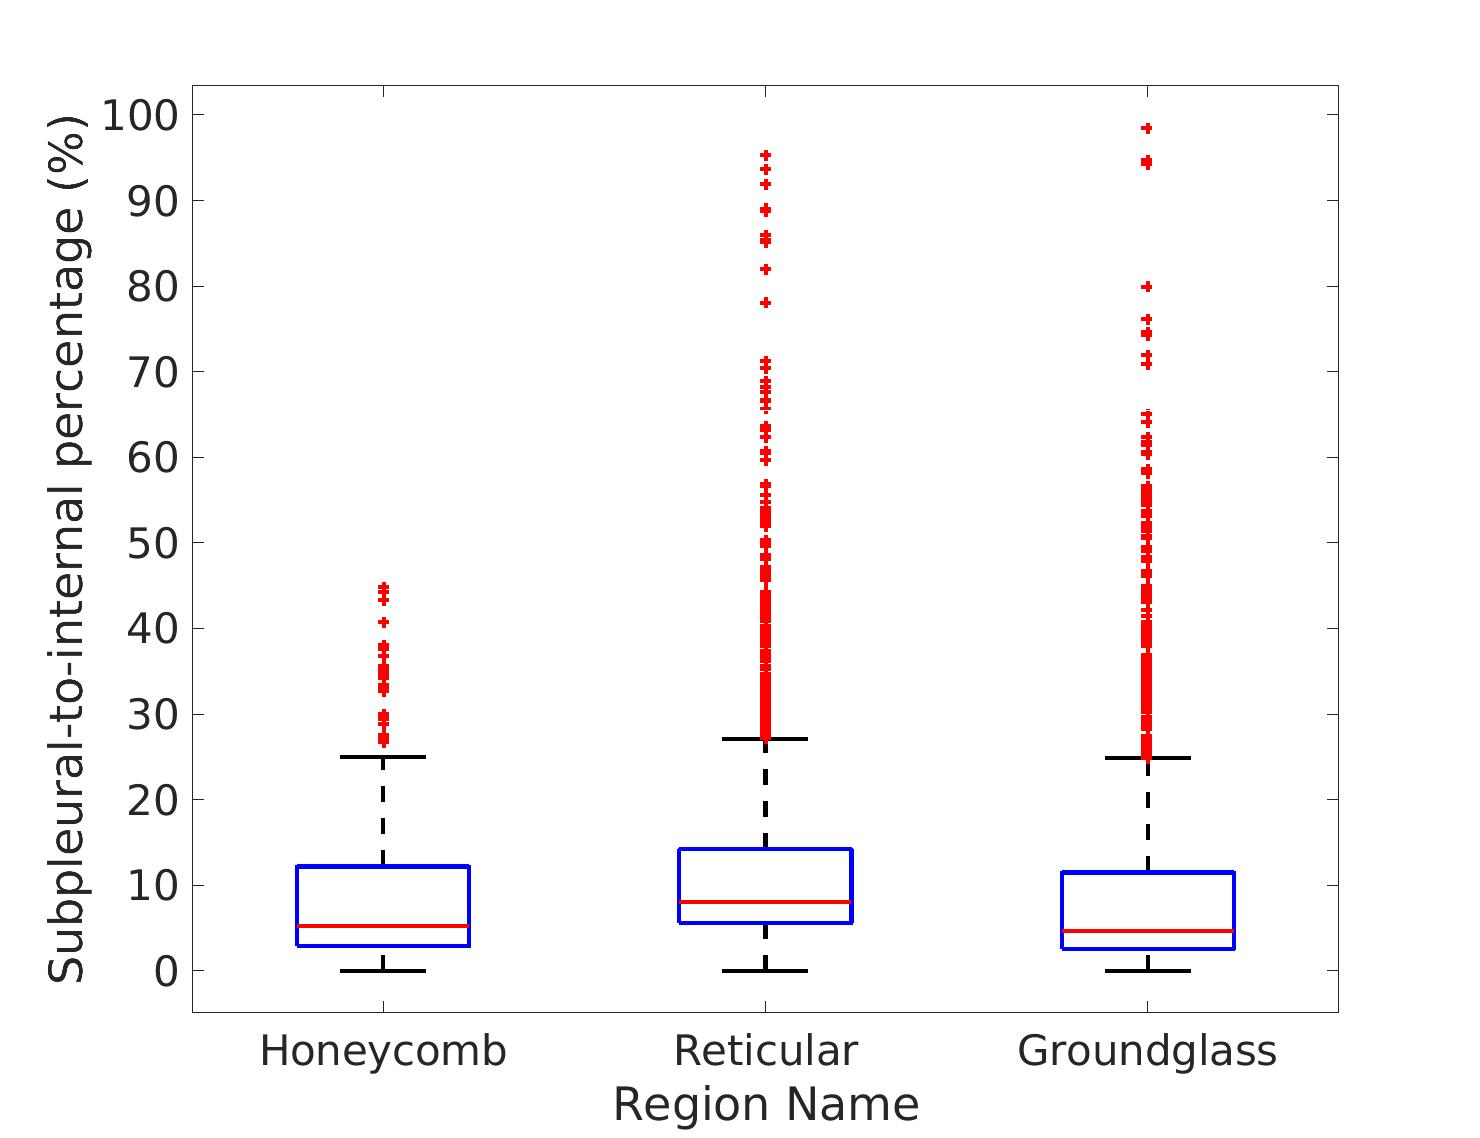
\includegraphics[width=\linewidth,trim={{.0\wd0} {.0\wd0} {.0\wd0} {.0\wd0}},clip]{QuantitativeAnalysis/Image/LeftLungDiseaseSubpleuralPercent.jpg} %trim={<left> <lower> <right> <upper>}, set the cut scale
  \caption{}
  \label{fig:DiseaseSubpleuralPercent-a} 
\end{subfigure} 
\hspace{.3in}
\begin{subfigure}{.5\linewidth}% set image scale
  \sbox0{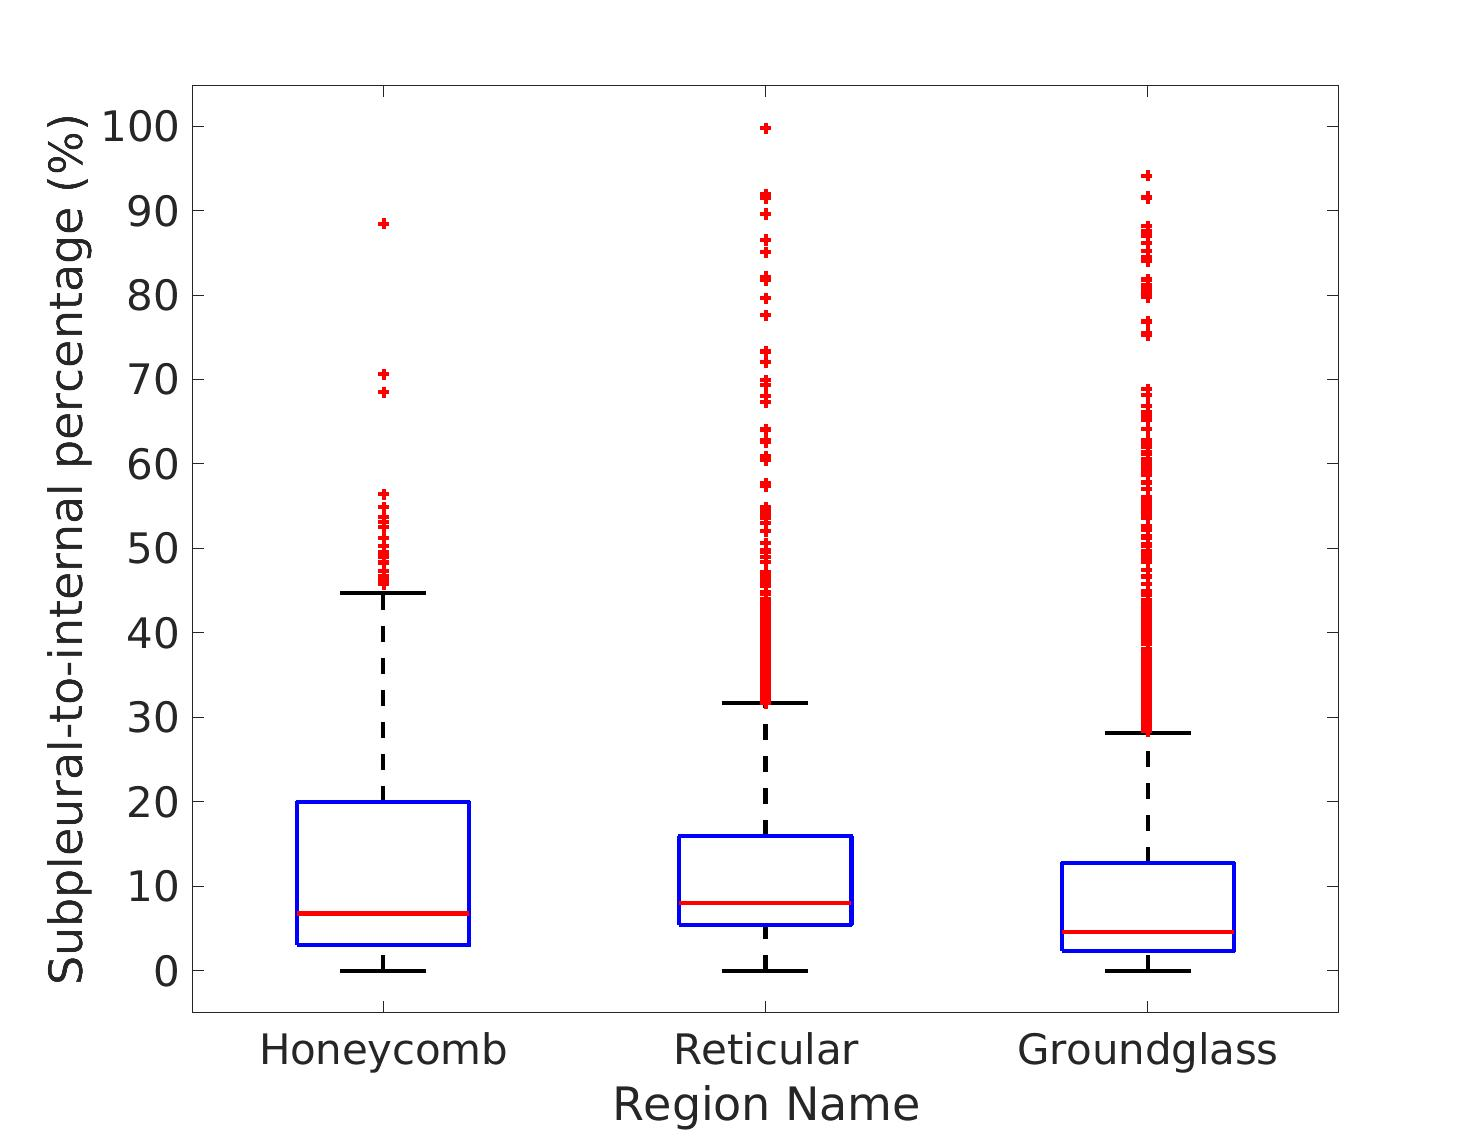
\includegraphics{QuantitativeAnalysis/Image/RightLungDiseaseSubpleuralPercent.jpg}}
  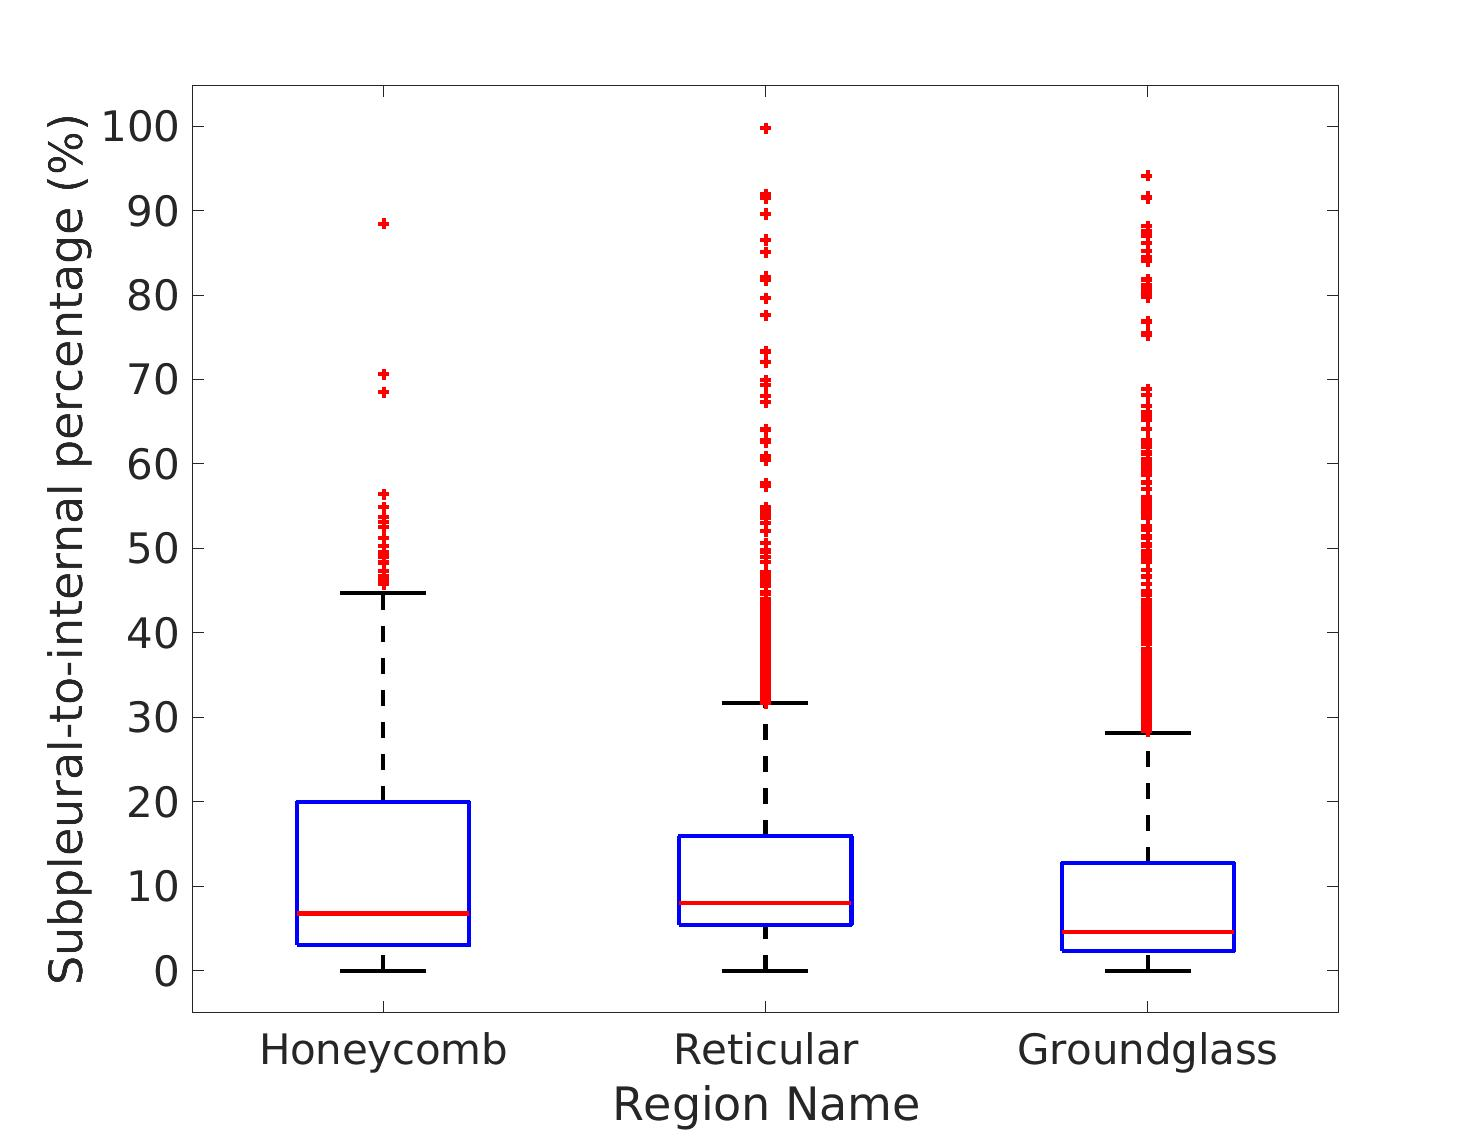
\includegraphics[width=\linewidth,trim={{.0\wd0} {.0\wd0} {.0\wd0} {.0\wd0}},clip]{QuantitativeAnalysis/Image/RightLungDiseaseSubpleuralPercent.jpg}
  \caption{}
  \label{fig:DiseaseSubpleuralPercent-b}
\end{subfigure}
\caption{ Subpleural-to-internal percentage of connected cluster of disease in IPF left and right lung. (a) Left lung. (b) Right lung.}
\label{fig:DiseaseSubpleuralPercent}
\end{figure}

\subsubsection{The change of tissue pattern over time}
Median survival time of patients with IPF is generally from 3 to 5 years. However, individual progression of disease is variable and how the characteristic disease pattern change over time (e.g. whether a disease region deteriorates and change to other tissue patterns or stay the same over time) still remains elusive. In our study, the classified data of all subjects and time points have been normalized to a standard lung shape (SSM, as introduced in Section \ref{DataNormalization}), thus making it possible for us to detect the disease change as time goes on by extracting the CT pattern of each voxel for different time points and mapping to a consistent framework.

Table \ref{tab:ChangeOverTimeLeft} and Table \ref{tab:ChangeOverTimeRight} show the quantitative results of how disease tissues (ground-glass and reticular) change over time. It describes the volume percentage of tissue CT patterns changing from the previous time point to the next time point (from ground-glass or reticular pattern to the other tissue CT patterns). Over 50\% of areas initially identified as ground-glass remain the same over time in both left and right lung, whereas other parts of ground-glass are subsequently classified as reticular or normal tissue as time goes by. As for reticular region, although quite a lot of reticular area doesn't change with the development of disease, a large proportion of reticular converts to ground-glass, especially in right lung (more than 50\% on average). In addition, around 10\%-30\% of reticular becomes normal region during this time. In general, the locations of abnormalities in IPF lung keep changing all the time. One kind of disease pattern may change to other patterns over time. Interestingly, some disease area may even change back to normal tissue, although a decline in lung function can be observed during this period.

\newgeometry{bottom=0.8cm} %set the left margin of page
\begin{landscape}
\begin{table}[p]
\centering
\caption{Change in classification of tissue CT pattern over time of left lung from one subject diagnosed with IPF (subject 6 with three time points) (\%).}
\label{tab:ChangeOverTimeLeft}
\begin{tabular}{c c c c c c c c c}
\hline
\quad & \quad & \bf{Ground-glass} &	\bf{Mild-LAA} &	\bf{Moderate-LAA} &	\bf{Normal} &	\bf{Reticular} &	\bf{Honeycomb} &	\bf{Severe-LAA}\\
\hline
\bf{Time1 - Time2} &	Ground-glass &	53.65 &	0.36 &	0	& 37.31 &	8.65 &	0 &	0.03\\
\quad & Reticular	& 29.76 &	3.01 &	0 &	28.41 &	38.82 &	0 &	0\\
\hline
\bf{Time2 - Time3} &	Ground-glass &	71.61 &	0.13 &	0.03 &	15.41 &	12.82 &	0 &	0\\
\quad & Reticular &	39.94 &	0.83 &	0 &	16.59 &	42.56 &	0.07 &	0\\
\hline
\bf{Time1 - Time3} &	Ground-glass &	70.01 &	0.83 &	0 &	20.80 &	8.35 &	0.01 &	0\\
\quad & Reticular &	37.97 &	4.73 &	0 &	15.49 &	41.81 &	0 &	0\\
\hline
\end{tabular}
\begin{tablenotes}
  \item[1] The time interval from time point 1 to time point 2 is 15 months, the time interval from time point 1 to time point 2 is 5 months, the time interval from time point 1 to time point 3 is 20 months.
\end{tablenotes}
\end{table}

\begin{table}[p]
\centering
\caption{Change in classification of tissue CT pattern over time of right lung from one subject (subject 6 with three time points) diagnosed with IPF (\%).}
\label{tab:ChangeOverTimeRight}
\begin{tabular}{c c c c c c c c c}
\hline
\quad & \quad & \bf{Ground-glass} &	\bf{Mild-LAA} &	\bf{Moderate-LAA} &	\bf{Normal} &	\bf{Reticular} &	\bf{Honeycomb} &	\bf{Severe-LAA}\\
\hline
\bf{Time1 - Time2} &	Ground-glass &	61.76 &	4.15 &	0.92 &	7.14 &	25.92 &	0 &	0.11\\
\quad & Reticular	& 47.61 &	6.88 &	0.01 &	11.10 &	34.37 &	0 &	0.03\\
\hline
\bf{Time2 - Time3} &	Ground-glass &	78.16 &	0.08 &	0.01 &	18.51 &	3.23 &	0 &	0.05\\
\quad & Reticular &	55.74 &	0.44 &	0 &	31.46 &	12.35 &	0.01 &	0\\
\hline
\bf{Time1 - Time3} &	Ground-glass &	79.98 &	1.82 &	1.63 &	12.82 &	3.45 &	0 &	0.30\\
\quad & Reticular &	65.80 &	3.28 &	0.02 &	19.40 &	11.33 &	0 &	0.16\\
\hline
\end{tabular}
\begin{tablenotes}
  \item[1] The time interval from time point 1 to time point 2 is 15 months, the time interval from time point 1 to time point 2 is 5 months, the time interval from time point 1 to time point 3 is 20 months.
\end{tablenotes}
\end{table}
\end{landscape}
\restoregeometry %reset margins of page

%%%%%%%%%%%%%%%%%%%%%%%%%%%%%%%%%%%%%%%%%%%%%%%%%%%%%%%%
\subsection{Volume analysis of IPF lungs} \label{VolumeAnalysis}
\subsubsection{The change of whole lung volume over time}
The volume of each classified tissue pattern in both left and right lung was calculated using the following equation:

\begin{equation}
V_{Region} = N \times R_x \times R_y \times R_z
\end{equation}

\noindent where N is the number of voxels of each tissue pattern, $R_{x}$, $R_{y}$ are the x, y resolution of the CT scan, and $R_{z}$ is the thickness of the CT scan. Then the whole volume of left and right lung was calculated as the sum of the volume of each CT pattern.

Table \ref{tab:WholeVolume} shows the whole volume of left and right lung of three subjects for each time point. It can be seen that the lung volumes of all these three IPF patients keep decreasing as a whole over time. 

\begin{table}[htbp]
\centering
\caption{Whole volume of left and right for each time point($1.0e 5 \ast mm^{3}$).}
\label{tab:WholeVolume}
\begin{tabular}{c c c c c}
\hline
\bf{Sub No.} & \bf{Time point} & \bf{Scan time}	& \bf{Left lung} &	\bf{Right lung}\\ 
\hline
IPF5 & Time point1 &  0 month & 1.73 & 1.49\\
\quad & Time point2 & 12 month & 1.58 & 1.31\\
\hline
IPF6 & Time point1 &	0 month &	2.41 &	3.47\\
\quad & Time point2 &	15 month &	2.13 &	3.01\\
\quad & Time point3 &	20 month &	2.06 &	3.09\\
\hline
IPF9 & Time point1 &	0 month &	1.35 &	1.49\\
\quad & Time point2 &	7 month &	1.22 &	1.43\\
\quad & Time point3 &	20 month &	1.23 &	1.53\\
\hline
\end{tabular}
\end{table}

\subsubsection{The change of tissue volume over time}
Currently, few studies have investigated the volume change of individual tissue pattern over time. In Section \ref{TissueQuantification}, it was demonstrated that the distribution of tissue abnormalities changes as time goes on. In this section, the volume percentages of normal tissue and classified fibrosis tissue (honeycomb, reticular and ground-glass) in left and right lung for each time point were calculated, and  results shown in Table \ref{tab:TissueVolumeLeft} and Table \ref{tab:TissueVolumeRight}.

\begin{table}[htbp]
\centering
\caption{The volume change of tissue CT pattern over time in left lung (\%).}
\label{tab:TissueVolumeLeft}
\begin{tabular}{c c c c c c c c}
\hline
\bf{Sub No.} & \bf{Time point} & \bf{Scan time}	& \bf{Normal} &	\bf{Honeycomb} & \bf{Reticular} & \bf{Ground-glass}\\ 
\hline
IPF5 & Time point1 &  0 month & 70.48 & 0 & 5.29 & 4.46\\
\quad & Time point2 & 12 month & 71.30 & 0.0300 & 3.53 & 7.96\\
\hline
IPF6 & Time point1 &	0 month &	15.98 &	0 & 0.98 & 1.46\\
\quad & Time point2 &	15 month &	21.28 &	0.0006 & 1.23 & 1.77\\
\quad & Time point3 &	20 month &	32.42 &	0.0014 & 1.78 & 3.69\\
\hline
IPF9 & Time point1 &	0 month &	85.21 &	0 & 0.65 & 1.63\\
\quad & Time point2 &	7 month &	90.69 &	0 & 0.43 & 2.56\\
\quad & Time point3 &	20 month &	88.22 &	0 & 0.37 & 2.08\\
\hline
\end{tabular}
\end{table}

\begin{table}[htbp]
\centering
\caption{The volume change of tissue CT pattern over time in right lung (\%).}
\label{tab:TissueVolumeRight}
\begin{tabular}{c c c c c c c c}
\hline
\bf{Sub No.} & \bf{Time point} & \bf{Scan time}	& \bf{Normal} &	\bf{Honeycomb} & \bf{Reticular} & \bf{Ground-glass}\\ 
\hline
IPF5 & Time point1 &  0 month & 58.44 & 0 & 8.59 & 13.95\\
\quad & Time point2 & 12 month & 59.39 & 0.0498 & 4.89 & 20.49\\
\hline
IPF6 & Time point1 &	0 month &	16.70 &	0.0064 & 0.77 & 1.49\\
\quad & Time point2 &	15 month &	22.52 &	0.0042 & 1.59 & 3.49\\
\quad & Time point3 &	20 month &	34.71 &	0.0073 & 1.05 & 6.05\\
\hline
IPF9 & Time point1 &	0 month &	94.73 &	0 & 0.79 & 1.16\\
\quad & Time point2 &	7 month &	95.12 &	0 & 0.54 & 1.52\\
\quad & Time point3 &	20 month &	91.06 &	0 & 0.17 & 0.69\\
\hline
\end{tabular}
\end{table}

Interestingly, Table \ref{tab:TissueVolumeLeft} and Table \ref{tab:TissueVolumeRight} show that the volume of tissue classified as normal does not keep decreasing all the time during the whole clinical course. For both subject IPF5 and IPF6, an increase in the volume of normal tissue over time can be observed, although the whole lung volume falls during this period (see Table \ref{tab:WholeVolume}). No regular tendency in volume change is found for abnormal tissues (honeycomb, reticular and ground-glass), which means the volume of tissue classified as fibrotic lesion can not necessarily be used as a predictor to assess the progression of disease.

\subsubsection{Lobe volume difference between old normal lungs and IPF lungs}
The lobe volume of IPF lung was compared to the older normal subjects described in Section \ref{DataNormalization}. In order to quantitatively analyze the lobe volume difference between the two groups, the volume proportion of each lobe was calculated:

\begin{equation}
 \label{eq:FissurePrediction1}
 P_{i} = \frac{V_{i}}{\sum_{i=1}^{5}V_i},
\end{equation}. 

\noindent where $V_{i}$ is the volume of each lobe with i=1 corresponding to left lower lobe, i=2 corresponding to left upper lobe, i=3 corresponding to right lower lobe, i=4 corresponding to right middle lobe and i=5 corresponding to right upper lobe. The difference in lobe volume proportions between IPF subjects and old normal subjects were compared statistically using t-test. Table \ref{tab:LobeVolumeAnalysis} shows the p values of the five lobes between the two groups.

\begin{table}[htbp]
\centering
\caption{P value of five lung lobes between IPF subjects and old normal subjects using t-test.}
\label{tab:LobeVolumeAnalysis}
\begin{tabular}{|l | c | c}
\hline
\bf{Lobe} & \bf{P-value} \\
\hline
Left lower lobe & 0.914 \\
\hline
Left upper lobe	& 0.904 \\
\hline
Right lower lobe	& 0.008 \\
\hline
Right middle lobe	& $\ll$ 0.001 \\
\hline
Right upper lobe	& 0.329 \\
\hline
\end{tabular}
\end{table}

The result shows that there is a significant difference of the volume proportion for right lower lobe and right middle lobe between IPF subjects and old normal subjects ($p<0.01$, $p<0.001$ respectively). 

In order to further compare lobe volumes between these two groups, the average lobe volume proportion among IPF subjects and among old normal subjects were then calculated respectively. The result is shown in Table \ref{tab:AverageLobeVolume}. It can be seen from Table \ref{tab:AverageLobeVolume} the IPF group has a lower average volume proportion for left lower lobe and right lower lobe compared to the value of old normal group. That may probably be caused by the increase in stiffness of lower lobe in IPF lungs, which relates to the basal appearance of fibrosis.

\begin{table}[htbp]
\centering
\caption{Average lobe volume proportion of IPF group and old normal group.}
\label{tab:AverageLobeVolume}
\begin{tabular}{| l | c | c |}
\hline
\bf{Lobe} & \bf{IPF} & \bf{Normal old} \\
\hline
Left lower lobe & 0.21 & 0.21\\
\hline
Left upper lobe	& 0.24 & 0.24\\
\hline
Right lower lobe	& 0.23 & 0.25\\
\hline
Right middle lobe	& 0.13 & 0.09\\
\hline
Right upper lobe	& 0.19 & 0.21\\
\hline
\end{tabular}
\end{table}

\subsection{SSM based shape analysis of IPF lungs} \label{SSMBasedAnalysis}
The SSM was used to quantitatively analyze the alterations in lung lobe shapes of patients with IPF. As previously described in Section \ref{DataNormalization}, 35 old normal subjects from AGING dataset were used as training data to construct the SSM which contained both lung surface and fissure surface. Through making use of PCA techniques, the shape variation of lung lobe was decomposed into a set of modes, and each mode represented one type of lung and fissure surface shape variation. Thus, each lung lobe shape can be described by a linear combination of the mode vector and its corresponding weight:

\begin{equation}
 \label{eq:FissurePrediction1}
 S_{new} = S_{mean} + \sum_{i=1}^L \mathbf{u}_i w_{i},
\end{equation}

\noindent where $S_{mean}$ is the average lobe shape model across all the training subjects, $\mathbf{u}_i (i = 1,2...L, L=34$ in this study) is the mode vector of shape variation which corresponds to the $i^{th}$ largest principle component from PCA, and $w_{i}$ is a weight factor given to each mode of variation. 

The lung lobe FE mesh of each IPF subject was then procrustes projected on to the average SSM after aligned to the reference model (details can be seen in Chapter 3, Section \ref{MeshPrediction}) The new weight values of all the shape modes $w_{new} = [w_{new1}, w_{new2},...,w_{newL}]$ (L = 35) were calculated from the projection. These mode weights can be used as quantitative indexes to analyze and compare the shape variation and difference between IPF and old normal lungs.

\subsubsection{Shape difference between IPF lungs and old normal lungs}

For SSM of old normal subjects, the first three shape modes explained over 30\% of the total variation in the training set. Therefore, the weight values of the first three modes were used as the measurement to compare the shape difference of lung lobe between old normal groups and IPF groups. Figure \ref{fig:ShapeDifference} shows the weight value distribution of the first three modes for IPF and old normal subjects. The p values of the first three shape modes between the two groups were calculated using t-test.

\begin{figure}[htbp] 
\centering
\begin{subfigure}{.65\linewidth}% set image scale
  \sbox0{\includegraphics{QuantitativeAnalysis/Image/Mode1AnalysisAgainstAge_NoTitle.png}} 
  \includegraphics[width=\linewidth,trim={{.0\wd0} {.0\wd0} {.0\wd0} {.0\wd0}},clip]{QuantitativeAnalysis/Image/Mode1AnalysisAgainstAge_NoTitle.png} %trim={<left> <lower> <right> <upper>}, set the cut scale
  \caption{Mode 1}
  \label{fig:ShapeDifference-a} 
\end{subfigure} 
\begin{subfigure}{.65\linewidth}% set image scale
  \sbox0{\includegraphics{QuantitativeAnalysis/Image/Mode2AnalysisAgainstAge_NoTitle.png}}
  \includegraphics[width=\linewidth,trim={{.0\wd0} {.0\wd0} {.0\wd0} {.0\wd0}},clip]{QuantitativeAnalysis/Image/Mode2AnalysisAgainstAge_NoTitle.png}
  \caption{Mode 2}
  \label{fig:ShapeDifference-b}
\end{subfigure}
\begin{subfigure}{.65\linewidth}% set image scale
  \sbox0{\includegraphics{QuantitativeAnalysis/Image/Mode3AnalysisAgainstAge_NoTitle.png}}
  \includegraphics[width=\linewidth,trim={{.0\wd0} {.0\wd0} {.0\wd0} {.0\wd0}},clip]{QuantitativeAnalysis/Image/Mode3AnalysisAgainstAge_NoTitle.png}
  \caption{Mode 3}
  \label{fig:ShapeDifference-c}
\end{subfigure}
\caption{ Shape differences between IPF subjects and old normal subjects of the first three modes (a) Mode 1 weight. (b) Mode 2 weight. (c) Mode 3  weight.}
\label{fig:ShapeDifference}
\end{figure}

%\begin{table}[htbp]
%\centering
%\caption{P value of the first shape modes between IPF subjects and old normal subjects using t-test.}
%\label{tab:WeightAnalysis}
%\begin{tabular}{|l | c |}
%\hline
%\bf{Mode} & \bf{P-value} \\
%\hline
%Mode 1 & $<$ 0.001 \\
%\hline
%Mode 2	& 0.194 \\
%\hline
%Mode 3	& 0.584 \\
%\hline
%\end{tabular}
%\end{table}

The results show that there is a significant difference of the first mode weight between IPF lungs and old normal lungs ($p<0.001$). However, for mode 2 and mode 3, no significant shape difference was observed between these two groups (p = 0.194 and p = 0.584, respectively). Figure \ref{fig:Mode1ShapeVariation} illustrates overall shape variation of the first mode with added different values of standard deviation to the mean shape model. The first shape mode accounts for over 20\% of the entire shape variation in old normal lungs. It is demonstrated from Figure \ref{fig:Mode1ShapeVariation} that the first mode relates to the largest change in the anteroposterior diameter of the lung with a lateromedial tilt towards the both apices, and is also associated with the ratio of apical and basal diameters. With the positive or negative standard deviation added to the mean shape model, there is a variation in the right anterior edge, the inferior lingular segment of the left superior lobe, the medial basal segment of the right middle lobe, and the left oblique fissure. In addition, there is a shape change in the ’roundness’ of the lateral surface in both left and right lung, and the variation in the distance of left and right lungs in the apex and base is also observed. As shown in Figure \ref{fig:ShapeDifference-a} and Figure \ref{fig:Mode1ShapeVariation}, the weight values of mode 1 for IPF subjects mostly distributed in negative zone, and the negative weight corresponds to a larger ratio of anteroposterior diameter to lung height compared to normal lungs. 

\newgeometry{left=1cm} %set the left margin of page
%\begin{landscape}
\begin{figure}[htbp]
\begin{subfigure}{6.0cm}
    \makebox[30pt]{\raisebox{40pt}{\rotatebox[origin=c]{0}{\minibox{$-3 \sigma$}}}}%
    \sbox0{\includegraphics{QuantitativeAnalysis/Image/PCA_Mode1_-3Front.png}}% get image width, trim={<left> <lower> <right> <upper>}
    \begin{overpic}[height=1.8in,trim={{.3\wd0} {.05\wd0} {.2\wd0} {.05\wd0}},clip]{QuantitativeAnalysis/Image/PCA_Mode1_-3Front.png}
    \end{overpic}
    \makebox[30pt]{\raisebox{40pt}{\rotatebox[origin=c]{0}{\minibox{$-1 \sigma$}}}}% \makebox:change left space, \raisebox: change upper space
    \begin{overpic}[height=1.8in,trim={{.3\wd0} {.05\wd0} {.2\wd0} {.05\wd0}},clip]{QuantitativeAnalysis/Image/PCA_Mode1_-1Front.png}
    \end{overpic}
		\makebox[30pt]{\raisebox{40pt}{\rotatebox[origin=c]{0}{\minibox{mean}}}}% \makebox:change left space, \raisebox: change upper space
    \begin{overpic}[height=1.8in,trim={{.3\wd0} {.05\wd0} {.2\wd0} {.05\wd0}},clip]{QuantitativeAnalysis/Image/PCA_Mode1_0Front.png}
    \end{overpic}
		\makebox[30pt]{\raisebox{40pt}{\rotatebox[origin=c]{0}{\minibox{$1 \sigma$}}}}%
    \sbox0{\includegraphics{QuantitativeAnalysis/Image/PCA_Mode1_-3Front.png}}% get image width, trim={<left> <lower> <right> <upper>}
    \begin{overpic}[height=1.8in,trim={{.3\wd0} {.05\wd0} {.2\wd0} {.05\wd0}},clip]{QuantitativeAnalysis/Image/PCA_Mode1_1Front.png}
    \end{overpic}
    \makebox[30pt]{\raisebox{40pt}{\rotatebox[origin=c]{0}{\minibox{$3 \sigma$}}}}% \makebox:change left space, \raisebox: change upper space
    \begin{overpic}[height=1.8in,trim={{.3\wd0} {.05\wd0} {.2\wd0} {.05\wd0}},clip]{QuantitativeAnalysis/Image/PCA_Mode1_3Front.png}
    \end{overpic}
    \caption{Anterior view}
		\label{fig:Mode1ShapeVariation-a}
\end{subfigure}\hspace{0.3cm}
\begin{subfigure}{4.8cm}
    \sbox0{\includegraphics{QuantitativeAnalysis/Image/PCA_Mode1_-3Front.png}}% get image width, trim={<left> <lower> <right> <upper>}
    \begin{overpic}[height=1.8in,trim={{.3\wd0} {.05\wd0} {.2\wd0} {.05\wd0}},clip]{QuantitativeAnalysis/Image/PCA_Mode1_-3Base.png}
    \end{overpic}
    \begin{overpic}[height=1.8in,trim={{.3\wd0} {.05\wd0} {.2\wd0} {.05\wd0}},clip]{QuantitativeAnalysis/Image/PCA_Mode1_-1Base.png}
    \end{overpic}
    \begin{overpic}[height=1.8in,trim={{.3\wd0} {.05\wd0} {.2\wd0} {.05\wd0}},clip]{QuantitativeAnalysis/Image/PCA_Mode1_0Base.png}
    \end{overpic}
    \sbox0{\includegraphics{QuantitativeAnalysis/Image/PCA_Mode1_-3Front.png}}% get image width, trim={<left> <lower> <right> <upper>}
    \begin{overpic}[height=1.8in,trim={{.3\wd0} {.05\wd0} {.2\wd0} {.05\wd0}},clip]{QuantitativeAnalysis/Image/PCA_Mode1_1Base.png}
    \end{overpic}
    \begin{overpic}[height=1.8in,trim={{.3\wd0} {.05\wd0} {.2\wd0} {.05\wd0}},clip]{QuantitativeAnalysis/Image/PCA_Mode1_3Base.png}
    \end{overpic}
    \caption{Basal view}
		\label{fig:Mode1ShapeVariation-b}
\end{subfigure}\hspace{0.3cm}
\begin{subfigure}{5.5cm}
    \sbox0{\includegraphics{QuantitativeAnalysis/Image/PCA_Mode1_-3Front.png}}% get image width, trim={<left> <lower> <right> <upper>}
    \begin{overpic}[height=1.8in,trim={{.3\wd0} {.05\wd0} {.2\wd0} {.05\wd0}},clip]{QuantitativeAnalysis/Image/PCA_Mode1_-3Back.png}
    \end{overpic}
    \begin{overpic}[height=1.8in,trim={{.3\wd0} {.05\wd0} {.2\wd0} {.05\wd0}},clip]{QuantitativeAnalysis/Image/PCA_Mode1_-1Back.png}
    \end{overpic}
    \begin{overpic}[height=1.8in,trim={{.3\wd0} {.05\wd0} {.2\wd0} {.05\wd0}},clip]{QuantitativeAnalysis/Image/PCA_Mode1_0Back.png}
    \end{overpic}
    \sbox0{\includegraphics{QuantitativeAnalysis/Image/PCA_Mode1_-3Front.png}}% get image width, trim={<left> <lower> <right> <upper>}
    \begin{overpic}[height=1.8in,trim={{.3\wd0} {.05\wd0} {.2\wd0} {.05\wd0}},clip]{QuantitativeAnalysis/Image/PCA_Mode1_1Back.png}
    \end{overpic}
    \begin{overpic}[height=1.8in,trim={{.3\wd0} {.05\wd0} {.2\wd0} {.05\wd0}},clip]{QuantitativeAnalysis/Image/PCA_Mode1_3Back.png}
    \end{overpic}
    \caption{Posterior view}
		\label{fig:Mode1ShapeVariation-c}
\end{subfigure}
\caption{PCA-derived shape variation of the first mode with added different values of standard deviation (-3$\sigma$, -1$\sigma$, $\mu$, 1$\sigma$, 3$\sigma$) to the mean shape model. (a) Anterior view. (b) Basal view. (c) Posterior view.}
\label{fig:Mode1ShapeVariation}
\end{figure}
%\end{landscape}
\restoregeometry

\subsubsection{Relationship between lung lobe shape and fibrosis extent}
In order to quantitatively investigate the impact of fibrosis extent on lung shape variation, the association of the first three modes with the overall volume percentage of fibrosis was measured by linear regression. Total fibrosis extent was represented by the sum of reticulation,  honeycombing and groud-glass opacification of both lungs. Figure \ref{fig:ShapeVSFibrosis} shows the behavior of the first three modes with respect to overall fibrosis percentage. Table \ref{tab:ShapeVSFibrosis} lists the P values and $R^2$ from linear regression.

From the result, the first shape mode shows a significant relationship with the percentage of fibrosis ($p<0.01$ ). With the increasement of the percentage of fibrosis, the weight value of mode 1 becomes lower negative which corresponds to a larger shape variation differ from the mean lung shape and normal lung shape (mainly locates in positive zone). In addition, it is observed that fibrosis lesion increases the ratio of anteroposterior diameter to the height of lung, which makes lung become ''fatter'' and ''shorter''. Therefore in general, the lung shape change in patient with IPF is strongly associated with the fibrosis extent, and the more extensive fibrosis the lung involves, the more ''abnormal'' the lung shape could become. 

\begin{table}[htbp]
\centering
\caption{P value of the first shape modes between IPF subjects and old normal subjects using t-test.}
\label{tab:ShapeVSFibrosis}
\begin{tabular}{|l | c | c |}
\hline
\bf{Mode} & \bf{P-value} & $\bf{R^2}$ \\
\hline
Mode 1 & $<$ 0.01 & 0.58 \\
\hline
Mode 2	& 0.77 & 0.01 \\
\hline
Mode 3	& 0.67 & 0.02 \\
\hline
\end{tabular}
\end{table}

\newpage

\begin{figure}[H] 
\centering
\begin{subfigure}{.65\linewidth}% set image scale
  \sbox0{\includegraphics{QuantitativeAnalysis/Image/Mode1AgainstFibrosis.png}} 
  \includegraphics[width=\linewidth,trim={{.0\wd0} {.0\wd0} {.0\wd0} {.0\wd0}},clip]{QuantitativeAnalysis/Image/Mode1AgainstFibrosis.png} %trim={<left> <lower> <right> <upper>}, set the cut scale
  \caption{Mode 1}
  \label{fig:ShapeVSFibrosis-a} 
\end{subfigure} 
\begin{subfigure}{.65\linewidth}% set image scale
  \sbox0{\includegraphics{QuantitativeAnalysis/Image/Mode2AgainstFibrosis.png}}
  \includegraphics[width=\linewidth,trim={{.0\wd0} {.0\wd0} {.0\wd0} {.0\wd0}},clip]{QuantitativeAnalysis/Image/Mode2AgainstFibrosis.png}
  \caption{Mode 2}
  \label{fig:ShapeVSFibrosis-b}
\end{subfigure}
\begin{subfigure}{.65\linewidth}% set image scale
  \sbox0{\includegraphics{QuantitativeAnalysis/Image/Mode3AgainstFibrosis.png}}
  \includegraphics[width=\linewidth,trim={{.0\wd0} {.0\wd0} {.0\wd0} {.0\wd0}},clip]{QuantitativeAnalysis/Image/Mode3AgainstFibrosis.png}
  \caption{Mode 3}
  \label{fig:ShapeVSFibrosis-c}
\end{subfigure}
\caption{ The Linear regression of the PCA-derived first three modes with respect to overall fibrosis percentage. (a) Mode 1 weight. (b) Mode 2 weight. (c) Mode 3  weight.}
\label{fig:ShapeVSFibrosis}
\end{figure}

%% Section 5
\section{Discussion} \label{QuantitativeDiscussion}
Individualized treatment strategies are urgently needed in clinical applications and are the ultimate goal of modern pulmonary medicine. Our quantitative analysis of IPF based on HRCT images has the potential to build a reliable relationship between imaging tissue-level biomarkers and clinical endpoints, furthermore is be able to help with medicine development or IPF disease research. Tissue density, tissue volume, spatial distribution of abnormalities and lung shape are all important indexes for representing a statistical progression of IPF disease. Through quantifying these features instead of qualitative evaluation, subjective errors could be avoided to offer a more consistent assessment.  

\subsubsection{Average statistical shape model provides a consistent measurement to quantify disease among different people and over the whole clinical course}
IPF is a progressive lung disease that has significant variable expression between different patients. Our SSM based quantitative method normalized a set of lungs of different shapes into a standard shape model, thus providing a convenient way to make a reliable comparison between different patients or within one patient of different time points. This method makes it possible to capture the disease variation across a population and describe the difference using objective indexes. Meanwhile, the progression of disease over time can be analyzed, and this will be helpful to predict the tendency of disease in clinical course. 

In addition, it is widely acknowledged that there should be some typical symptoms occurring on average 1-2 years before a definite clinical diagnosis with IPF, and some radiographic evidence of IPF may even be found before symptoms occur \citep{raghu2011official, devaraj2014imaging}. This ‘subclinical’ period of disease is very important for an early diagnosis of IPF disease. Our SSM based method makes it possible to compare IPF diseased lungs to old normal subjects. Through combining the disease progression of successive time points with the difference compared to old normal lungs, we can get a whole prediction of disease prognosis in IPF lungs from normal state to severe injured state. It is helpful for clinician to recognize abnormalities in a ‘normal’ lung at subclinical stage, and is also a further goal of our research in the next stage. 

\subsubsection{Tissue density can be used as a quantitative biomarker of IPF, but tissue volume not}
The density analysis conducted in this chapter shows that tissue density of different tissue CT patterns fluctuate within different ranges. There is a significant difference of average density between normal lung parenchyma and fibrosis areas (honeycomb, reticular and ground-glass), whereas emphysema usually has the lowest tissue density (Hounsfield unit lower than -950) compared to normal and fibrosis. Therefore, tissue density can be used as a potential biomarker to distinguish the disease regions from other lung parenchyma. As for tissue volume of each CT pattern, no continuous tendency of the volume of both normal tissue and abnormal tissue was found to demonstrate a correlation with time. Therefore, the change of tissue volume can not be used as a reliable biomarker to interpret the progression of disease.

\subsubsection{The shape of basal part of IPF lung is significantly different from old normal lung and correlates with fibrosis extent}
The first shape mode of SSM is significantly different between IPF subjects and old normal subjects and strongly correlates with the percentage of fibrosis. The first shape mode corresponds mainly to the anteroposterior diameter of lung which results in a variation of diaphragm. This shape change of diaphragm can be explained by the spatial distribution of tissue abnormalities. The basal and peripheral performance of disease may increase the stiffness of the lower part of lung, thus having a impact on the movement of diaphragm when breathing. Furthermore, fibrosis extent in IPF lungs is found to be related to the ratio of anteroposterior diameter to the height of lung. A larger area of fibrosis is usually correlated with a larger ratio of anteroposterior diameter to the height of lung. This ''compression effect'' on the lung shape may be associated the reduction in tissue compliance of IPF lungs caused by fibrosis. Specifically, since the IPF subjects and old normal subjects used in this chapter were all acquired at the end of inspiration, the lower tissue compliance caused by fibrosis lesion will influence the expansion of the lung during inhalation if derived by a normal muscle pressure of respiration, therefore may have an effect on the lung shape. In addition, it is demonstrated in the lobe volume analysis that IPF lung has a lower average volume proportion for left lower lobe and left upper lobe, which may be also caused by the ''compression effect'' of the lower lobe in IPF lungs.

\subsubsection{The quantification of combined IPF and emphysema is the difficulty and emphasis in the future work}
Combined IPF and emphysema (CPFE) has been mentioned and defined in the past ten years \citep{cottin2005combined,meltzer2008idiopathic}. Some researchers suggest that CPFE should be regarded as a distinct clinical entity other than emphysema or IPF alone, since it has a characteristic pulmonary function feature different from pure emphysema or IPF. It is commonly believed that CPFE is strongly associated with heavy smokers, severe dyspnea on exertion and impaired gas exchange, and emphysema usually happens in the upper lobe whereas IPF disease tends to appear in the lower lobe \citep{lin2015combined} which is consistent with the result of our analysis. However, whether the presence of the two diseases developing in parallel is still unknown \citep{cottin2005combined, king2011idiopathic, lin2015combined}. In the future work, the image based analysis result will be used as quantitative indexes in a lung functional modeling, which could help understand the relationship between the two diseases and the impact of emphysema on IPF.

\section{Summary}
In this chapter, we analyzed and characterized IPF classified tissue over time using quantitative methods. The result shows that fibrosis had higher tissue density compared with normal tissue, and presented predominantly basally and peripherally. In contrast, emphysema had lower tissue density and mostly located in upper lobes. The first principal SSM mode ($>20\%$ of the shape variation in normal lungs) was significantly different between IPF and normal and strongly correlated with fibrosis extent in IPF lungs. This quantitative analysis provides consistent potential tissue-level markers which will be used to guide the computational modeling of IPF lungs in the next chapter.





